\documentclass[12pt, twoside, table]{extarticle} % book, report, and article ; extarticle so you could use 14pt as a size

% mendeley para referenceias sugestão da Inês

% No VSC: CTRL  ALT + J para ir do codigo para o pdf
% CTRL + Click para ir do pdf para o codigo

% na pagina principal deve ficar centrado
\usepackage{titling}
\renewcommand\maketitlehooka{\null\mbox{}\vfill}
\renewcommand\maketitlehookd{\vfill\null}

% so you can use \begin{sortedlist}
% https://tex.stackexchange.com/questions/121489/alphabetically-display-the-items-in-itemize    
\usepackage{datatool}% http://ctan.org/pkg/datatool
\newcommand{\sortitem}[1]{%
  \DTLnewrow{list}% Create a new entry
  \DTLnewdbentry{list}{description}{#1}% Add entry as description
}
\newenvironment{sortedlist}{%
  \DTLifdbexists{list}{\DTLcleardb{list}}{\DTLnewdb{list}}% Create new/discard old list
}{%
  \DTLsort{description}{list}% Sort list
  \begin{itemize}%
    \DTLforeach*{list}{\theDesc=description}{%
      \item \theDesc}% Print each item
  \end{itemize}%
}

\newcommand{\source}[1]{\vspace{-3pt} \caption*{ Fonte: {#1}} } % to add source to images

% ----- subsubsubsection
\usepackage{titlesec}

\titleclass{\subsubsubsection}{straight}[\subsection]

\newcounter{subsubsubsection}[subsubsection]
\renewcommand\thesubsubsubsection{\thesubsubsection.\arabic{subsubsubsection}}
\renewcommand\theparagraph{\thesubsubsubsection.\arabic{paragraph}} % optional; useful if paragraphs are to be numbered

\titleformat{\subsubsubsection}
  {\normalfont\normalsize\bfseries}{\thesubsubsubsection}{1em}{}
\titlespacing*{\subsubsubsection}
{0pt}{3.25ex plus 1ex minus .2ex}{1.5ex plus .2ex}

\makeatletter
\renewcommand\paragraph{\@startsection{paragraph}{5}{\z@}%
  {3.25ex \@plus1ex \@minus.2ex}%
  {-1em}%
  {\normalfont\normalsize\bfseries}}
\renewcommand\subparagraph{\@startsection{subparagraph}{6}{\parindent}%
  {3.25ex \@plus1ex \@minus .2ex}%
  {-1em}%
  {\normalfont\normalsize\bfseries}}
\def\toclevel@subsubsubsection{4}
\def\toclevel@paragraph{5}
\def\toclevel@paragraph{6}
\def\l@subsubsubsection{\@dottedtocline{4}{7em}{4em}}
\def\l@paragraph{\@dottedtocline{5}{10em}{5em}}
\def\l@subparagraph{\@dottedtocline{6}{14em}{6em}}
\makeatother

\setcounter{secnumdepth}{4} % Sections depth with numbering
\setcounter{tocdepth}{2} % Sections depth in the TOC
% ----- subsubsubsection

% allow deeper nesting
% https://stackoverflow.com/questions/1935952/maximum-nesting-level-of-lists-in-latex
\usepackage{enumitem}
\setlistdepth{9}
\setlist[itemize,1]{label=$\bullet$}
\setlist[itemize,2]{label=$\bullet$}
\setlist[itemize,3]{label=$\bullet$}
\setlist[itemize,4]{label=$\bullet$}
\setlist[itemize,5]{label=$\bullet$}
\setlist[itemize,6]{label=$\bullet$}
\setlist[itemize,7]{label=$\bullet$}
\setlist[itemize,8]{label=$\bullet$}
\setlist[itemize,9]{label=$\bullet$}
\renewlist{itemize}{itemize}{9}

% make new sections start on odd pages even on oneside article document, needs to be after the subsubsubsection redefinition
% https://tex.stackexchange.com/a/51928
%\usepackage[strict]{changepage}% http://ctan.org/pkg/changepage
%\newcommand{\evenpagesection}{%
%  \global\let\oldsection\section
%  \renewcommand\section{%
%    \clearpage\checkoddpage%
%    \ifoddpage\null\clearpage\fi%
%    \oldsection
%  }%
%}
%\evenpagesection % activate starting sections on an even page
% new method
% https://tex.stackexchange.com/questions/443453/start-sections-on-odd-pages-article-class
\usepackage{blindtext}
\usepackage{etoolbox}
\pretocmd{\section}{\cleardoublepage}{}{}

% -------------------------------------------------------------------
% Pacotes básicos
\usepackage[main=portuguese, english]{babel}										% Idioma a ser usado
% Trocar "english" para "portuguese" para artigos escritos em língua portuguesa (brazil também dá) 
\usepackage[utf8]{inputenc}										% Escrita de caracteres acentuados e cedilhas - 1
\usepackage[T1]{fontenc}										% Escrita de caracteres acentuados + outros detalhes técnicos fundamentais
% -------------------------------------------------------------------
% Pacotes matemáticos
\usepackage{amsmath,amsfonts,amssymb,amsthm,cancel,siunitx,
calculator,calc,mathtools,empheq,latexsym}
% -------------------------------------------------------------------
% Pacotes para inserção de figuras e subfiguras
\usepackage{subfig,epsfig,tikz,float}		            % Packages de figuras. 
\usepackage{pgfplots} % For graphs and plots
\pgfplotsset{compat=1.18} % specify the version of the pakage bc its updated frequently
% -------------------------------------------------------------------
% Pacotes para inserção de tabelas
\usepackage{booktabs,multicol,multirow,tabularx,array}          % Packages para tabela
\usepackage{xcolor}
\usepackage{tabularray} % usar o tblr (better tabularx alternative)
% -------------------------------------------------------------------
\usepackage{pgfgantt} % gantt charts
% -----------------------------------------------------------------
\usepackage{fancyhdr} % For copyright notice at the end
% -----------------------------------------------------------------
\usepackage{csquotes}
\usepackage{verbatim} % so you can use \begin{comment} adn \end{comment}
\usepackage{graphicx}
\usepackage{lipsum}% http://ctan.org/pkg/lipsum
\usepackage{svg}  % For including SVG images with \includesvg[width=0.4\textwidth]{imgs} instead of \includegraphics[...

\usepackage[style=ieee, backend=biber]{biblatex} % \usepackage{biblatex} % to use .bib files for references
\addbibresource{references.bib}  % Specify the path to your .bib file

\usepackage{pmboxdraw}
\usepackage{listings} % for code
\usepackage{microtype} % For better justification?

% To attach pdfs
\usepackage{pdfpages}
\pdfminorversion=7 % allow more recent pdfs

%Select font:
\usepackage{times} % Times New Roman (?)
%\usepackage{carlito} % Arial?
\usepackage{romannum} % Use \Romannum{17} or \romannum{17}

% Paragraphs
%\setlength{\parskip}{\baselineskip}%
%\setlength{\parskip}{8pt}
\usepackage[skip=10pt plus1pt, indent=20pt]{parskip} % makes TOC look better as well
% redefining maketitle to have the logos - https://tex.stackexchange.com/questions/357769/add-a-picture-before-book-title
\usepackage{titling}

% To center the first page 
% https://tex.stackexchange.com/questions/57158/centered-title-page-in-twoside-report
\usepackage[margin=1in,bindingoffset=.2in]{geometry} %% Remove showframe in your document

\usepackage{xurl} % to make links in the bibliography not overflow

\usepackage[colorlinks=true, allcolors=blue]{hyperref} % should be last package
\usepackage{attachfile2} % needs to be after hyperref?

% margins
% normally you shouldn't mess with margins, refer to here why they're usually so big: https://tex.stackexchange.com/questions/71172/why-are-default-latex-margins-so-big
% \usepackage{geometry}
% sizes taken from ISEC thesis template
% \geometry{paper=a4paper, 
% 	lmargin=2.54cm, rmargin=2.54cm, 
% 	tmargin=2.54cm, bmargin=2.54cm }
% Margins like Word:
% https://tex.stackexchange.com/questions/35892/latex-optimal-settings-for-ms-word-like-document
% \usepackage[tmargin=1in,bmargin=1in,lmargin=1.25in,rmargin=1.25in]{geometry}.

% Make the document black/dark, looking good
%\pagecolor{black}
%\color{white}%
%\definecolor{mylinkcolor}{HTML}{81cfff} % same that google uses
%\hypersetup{
%  colorlinks=true,
% allcolors=mylinkcolor
%}

\linespread{1.15}

% To compile only part
% \includeonly{cover/cover}

\begin{document}

  
\begin{titlepage}
  \thispagestyle{empty} % removes numbering from first page
  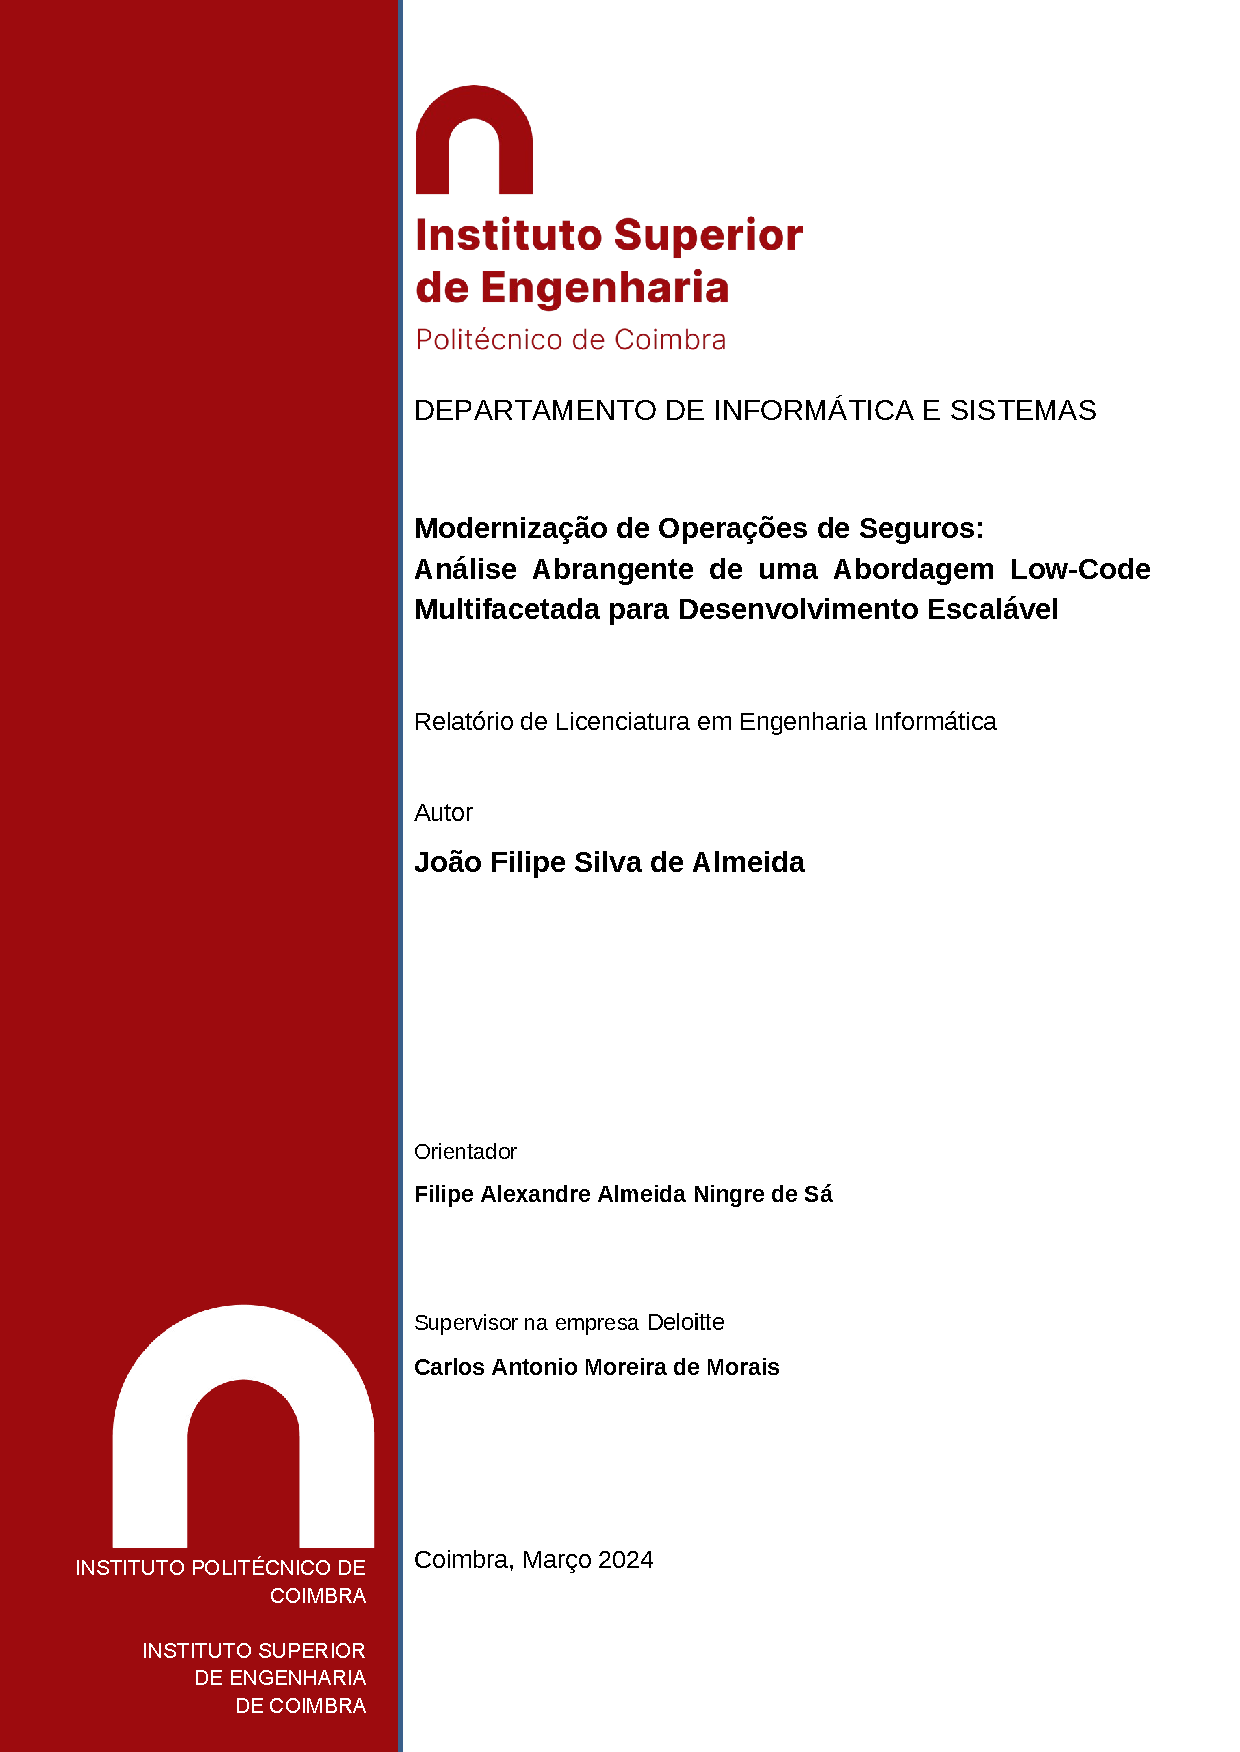
\includepdf[fitpaper=true]{src/cover/capa.pdf}
\end{titlepage}

\begin{comment}

\definecolor{redstrip}{RGB}{220,20,60}
\definecolor{bordergray}{RGB}{150,150,150}

\AddToShipoutPictureBG*{%
  \AtPageLowerLeft{%
    \color{redstrip}%
    \rule{0.33\paperwidth}{\paperheight}%
    \color{bordergray}%
    \put(0,0){\makebox(0,0)[l]{\rule[-\paperheight]{3pt}{2\paperheight}}}%
    \put(5,-\paperheight+5){\includegraphics[width=2cm]{example-image}} % Adjust the position and size of the image
  }%
}

\begin{tikzpicture}[overlay, remember picture]
  \node[anchor=north west, %anchor is upper left corner of the graphic
        xshift=5cm, %shifting around
        yshift=-5cm] 
       at (current page.north west) %left upper corner of the page
       {\includegraphics[width=5cm]{src/cover/LogoISEC2.png}}; 
  \end{tikzpicture}

\begin{tikzpicture}[remember picture,overlay]
  % Desenhar a parte vermelha
  \fill[red] (current page.north west) rectangle ++(0.33\paperwidth,-\paperheight);
  % Adicionar a imagem dentro da parte vermelha
  \node[anchor=south west, inner sep=0] at (current page.south west) {
      \begin{minipage}[b]{0.33\paperwidth}
          \includegraphics[width=\linewidth]{example-image}
      \end{minipage}
  };
\end{tikzpicture}



\definecolor{redstrip}{RGB}{220,20,60}
\definecolor{bordergray}{RGB}{150,150,150}

\AddToShipoutPictureBG*{%
  \AtPageLowerLeft{%
    \color{redstrip}%
    \rule{0.33\paperwidth}{\paperheight}%
    \color{bordergray}%
    \put(0,0){\makebox(0,0)[l]{\rule[-\paperheight]{3pt}{2\paperheight}}}%
    \put(5,-\paperheight+5){\includegraphics[width=2cm]{example-image}} % Adjust the position and size of the image
  }%
}


\title{Modernização de Operações de Seguros: \\
Análise Abrangente de uma Abordagem Low-Code Multifacetada para Desenvolvimento Escalável}

\author{%
  Almeida, João Filipe\\
  \texttt{a2020144466@isec.pt}
}

\date{} % remove date

\maketitle

\end{comment}




  \section{Resumo}\label{sec:resumo}

    Este relatório descreve um trabalho onde se aborda a modernização das operações de seguros através da implementação de uma abordagem \textit{low-code}, com foco na plataforma OutSystems. Ao longo do estágio curricular, foram enfrentados desafios significativos, desde a adaptação a novas tecnologias até à integração eficiente de sistemas existentes. A análise abrangente do desenvolvimento \textit{low-code} multifacetado destaca os benefícios e as considerações essenciais ao utilizar esta abordagem no contexto específico das operações de seguros. 
    
    Este relatório visa contribuir para a compreensão do impacto do desenvolvimento \textit{low-code} na área de seguros, destacando as vantagens e desvantagens das várias tecnologias, os seus competidores e como se interligam entre si, nomeadamente Azure, MongoDB, Nuxeo e competidores.

    Toda a descrição do processo acontecerá num contexto de um estágio curricular cujo propósito foi o avanço académico do estagiário na área de Tecnologias de Informação e cujas tarefas estenderam-se entre a correção e reporte de defeitos da aplicação, a análise e acompanhamento dos utilizadores nos seus incidentes e a execução de terceiras tarefas como outras que tenham sido necessárias ou requisitadas, bem como a tentativa de constante automação e aprimoramento dos processos usados nas resoluções.  


    \medskip
    \noindent
    {\small{\bf Palavras-chave:} 
    outsystems, \textit{low-code}, seguros, seguradoras, mongodb, azure, nuxio, subscritor, corretor, contrato, atlas, service center, lifetime, service studio, ServiceNow}

  \begin{otherlanguage}{english}
    \section{Abstract}\label{sec:abstract}

    This report describes a project that addresses the modernization of insurance operations through the implementation of a low-code approach, focusing on the OutSystems platform. Throughout the academic internship, significant challenges were encountered, ranging from adapting to new technologies to efficiently integrating existing systems. The comprehensive analysis of multifaceted low-code development highlights the benefits and essential considerations when employing this approach in the specific context of insurance operations.
    
    This report aims to contribute to the understanding of the impact of low-code development in the insurance sector, highlighting the advantages and disadvantages of various technologies, their competitors, and how they interconnect with each other, namely Azure, MongoDB, Nuxeo, and competitors.
    
    The entire process description occurs within the context of a curricular internship aimed at advancing the intern's academic knowledge in the field of Information Technologies. Tasks included bug correction and reporting, analysis, and user support in incidents, as well as the execution of third-party tasks as needed or requested, along with ongoing attempts at process automation and improvement.
    
    \medskip
    \noindent
    {\small{\bf Keywords:}
    outsystems, low-code, insurance, mongodb, azure, nuxio, underwriter, broker, contract, atlas, service center, lifetime, service studio, ServiceNow}
\end{otherlanguage}

  \section{Epígrafe}\label{sec:epigrafe}
\begin{quote}
    \textit{``A ciência é mais que um corpo de conhecimento, é uma forma de pensar, uma forma cética de interrogar o universo, com pleno conhecimento da falibilidade humana.''}
\end{quote}
\begin{flushright}
Carl Sagan
\end{flushright}


  \section{Agradecimentos}\label{sec:agradecimentos}

    Quero aproveitar esta oportunidade para expressar a minha sincera gratidão a todos os que contribuíram de alguma forma para o desenvolvimento e conclusão deste projeto.

    Gostaria de expandir os meus agradecimentos ao meu orientador na empresa Deloitte, Carlos Morais, pelo valioso suporte, orientação e contribuições fundamentais ao longo deste projeto. O seu excelente acompanhamento, a sua constante e perspicaz avaliação, assim como a gestão dos diferentes membros da equipa com variadas personalidades e capacidades fez-me crescer como profissional e vai sem dúvida deixar um impacto duradouro na minha futura carreira profissional. \newline
    Sinto-me igualmente endividado ao meu orientador universitário, Filipe Sá, que não só estimo como supervisor cujo conhecimento e proficiência na área de informática de sistemas e imaculado historial na orientação de estágios me permitiram manter um alto rigor e qualidade na elaboração do relatório, e sinto-me bastante privilegiado por ter a oportunidade de aproveitar o seu aconselhamento cujos contributos foram essenciais para o sucesso desta iniciativa.

    Estendo os meus agradecimentos a toda a equipa da Deloitte, incluindo os membros da equipa em que fui integrado, João Freitas, Nuno Gaio, Andreia Gomes, Liliana Ferreira, Márcio Costa, Jorge Tavares e Laisa Lamir, pela colaboração, dedicação e trabalho em equipa excecionais com os quais sempre tive uma relação próxima e acolhedora, amplio os meus agradecimentos ainda aos restantes membros das equipas do projeto com quem sempre me senti à vontade para inquirir acerca de quaisquer dúvidas e sempre estive confortável para partilhar qualquer questão, e sempre me ajudaram no crescimento dentro da empresa e no projeto.

    Agradeço ainda a todos na comunidade académica do ISEC, desde professores e docentes até colegas e alunos, pela troca de conhecimentos e experiências enriquecedoras ao longo deste percurso educacional que me deixaram apenas com um grande carinho pela instituição e por todas as experiências que me proporcionaram, nunca esquecerei o meu tempo de grande aprendizagem e desenvolvimento que tive o prazer de passar no ISEC e considero-me bastante sortudo por ter tido esta oportunidade, obrigado a todos!
  \newpage


  % \newpage % use new page when a chapter is over, use pagebreak when a chapter isn't over
  \tableofcontents 
  \listoffigures
  \listoftables

  \section{Abreviaturas}\label{sec:abreviacoes} % Abreviações
    % Already in alphabetical order                                    
    \begin{sortedlist}
        \sortitem{ISEC — Instituto Superior de Engenharia de Coimbra}
        \sortitem{CMMI — \textit{Capability Maturity Model Integration}}
        \sortitem{PL/SQL — \textit{Procedural Language/Structured Query Language}}
        \sortitem{SQL — \textit{Structured Query Language}}
        \sortitem{MS — Microsoft}
        \sortitem{UML — \textit{Unified Modeling Language}}
        \sortitem{IaaS — \textit{Infrastructure as a Service}}
        \sortitem{PaaS — \textit{Platform as a Service}}
        \sortitem{SaaS — \textit{Software as a Service}}
        \sortitem{SO — Sistema Operativo}
        \sortitem{GWP — \textit{Gross written premium}}
        \sortitem{OS — OutSystems}
        \sortitem{AD Factory — \textit{Application Development Factory}}
        \sortitem{VM — \textit{Virtual Machine}(Máquina Virtual)}
        \sortitem{UI — \textit{User Interface}}
        \sortitem{AWS — Amazon Web Services}
        \sortitem{DB — \textit{Data Base}}
        \sortitem{US — \textit{User Story}}
        \sortitem{BA — \textit{Business Analysts}}
        \sortitem{AMS — \textit{Application Managed Services}}
        \sortitem{UMR — \textit{Unique Market Reference}}
        \sortitem{UW — \textit{Underwriter}}
        \sortitem{FO — \textit{Firm Order}}
        \sortitem{MF — \textit{Master Facility}}
        \sortitem{MRC — \textit{Mutual Responsibility Contract}}
        \sortitem{TI — Tecnologia de Informação}
        \sortitem{URL — Uniform Resource Locator}
        \sortitem{MQL — \textit{MongoDB Query Language}}
    \end{sortedlist}

  % -----------------------------------------------------------------

  \setcounter{secnumdepth}{4} % Sections have numbering again up to the subsub, paragraph section

  \section{Introdução}\label{sec:introducao}
    \pagenumbering{arabic} % Change the numbering for the mainmatter

    Este relatório descreve o projeto e atividades desenvolvidas durante o estágio curricular do autor para a conclusão da sua licenciatura realizada no Instituto Politécnico de Coimbra, realizado na Deloitte Touche Tohmatsu Limited. O percurso divide-se em duas fases, uma primeira direcionada à formação e integração do estagiário e a segunda direcionada ao projeto, sua infraestrutura e às diferentes tarefas resolvidas no âmbito deste.

    Entre as formações ministradas incluem-se PL/SQL, Java, Excel, SQL e Modelação, Agile e Scrum, OutSystems, Azure, OWASP e MongoDB. Além disso, foram oferecidas formações de curta duração abordando tópicos como Boas Práticas de Desenvolvimento, Banca, Seguros, \textit{Getting Things Done} e \textit{Capability Maturity Model Integration} (CMMI).

    A aplicação prática de tecnologias no estágio passou pela utilização de ferramentas como OutSystems, Excel, SQL, MongoDB Query Language (MQL), Azure e até a programação em Python. Detalhes mais específicos sobre estas experiências e as suas aplicações serão descritos nos capítulos subsequentes.

    \subsection{ISEC}\label{subsec:isec}
        % Falar do ISEC
        % Podes falar um pouco sobre a cidade
    
        O \href{https://isec.pt/}{Instituto Superior de Engenharia de Coimbra} (ISEC) É uma subdivisão do \href{https://ipc.pt/}{Instituto Politécnico de Coimbra} (IPC) dedicada às engenharias do instituto.
    
        É uma instituição com várias décadas de história, sendo possível traçar relação ao Instituto Industrial e Comercial de Coimbra fundado em 1921\cite{iscac} fundado com a intenção de atender à crescente necessidade de engenheiros especializados. Foi dividida no Instituto Superior de Engenharia de Coimbra e no Instituto Comercial de Coimbra devido ao Decreto-Lei n.º 830\cite{iscac} em 1974 que converteu os institutos industriais em institutos superiores de engenharia. Foi apenas em 1988\cite{wiki-isec} através do Decreto-Lei nº389/88\cite{decreto389/88} que foi integrado no Ensino Superior Politécnico, consolidando a instituição ainda mais como uma das escolas principais de engenharia em Portugal, continuando até hoje a expandir a sua oferta formativa de modo a se adaptar à indústria bastante volátil.
    
        O ISEC oferece uma vasta gama de cursos a vários níveis académicos tendo CTeSPs, licenciaturas e mestrados e cobrindo vários ramos de engenharia, alguns destes cursos são: Bioengenharia, Engenharia Biomédica, Engenharia Eletrotécnica e de Computadores, Engenharia Eletromecânica, Engenharia Civil, Engenharia e Gestão Industrial e muitos mais, destingindo-se devido ao seu método prático de aprendizagem e à sua proximidade com o mercado de trabalho, oferecendo bastantes oportunidades de contacto com empresas, muitas vezes sendo intrínseco ao currículo do curso.
    
        A vida no campus é também bastante rica, havendo uma abundância de atividades extra curriculares e associações académicas que contribuem para o desenvolvimento das bastante procuradas no mercado ``Soft Skills'', destas atividades fazem parte: A Tuna do ISEC, o EcoCampus do ISEC, a Associação de Estudantes, a Comissão de Estudantes, o Serviço de Apoio à Praxe (SAP), várias instalações e equipas de desporto como a equipa de futebol do IPC, e eventos mais chegados às empresas como a Feira de Engenharia de Coimbra (FENGE), o Fikalab ou o PoliEmpreende, entre outros. Estimulando assim o pensamento crítico e o crescimento social dos alunos, ajudando também na construção de conexões relevantes para o mercado de trabalho.
    
        A própria cidade de Coimbra é bastante acolhedora academicamente sendo frequentemente referida como ``A cidade dos estudantes'', é casa da universidade mais antiga de Portugal\cite{universidade-coimbra} bem como a mais antiga associação de estudantes do país\cite{wiki-associacao}. Providenciando assim um ambiente académico que incita à criatividade e à exploração.
    
        Em conclusão, o ISEC é uma escola de engenharia bastante prestigiada e procurada por empresas de todo o país, com sólidos princípios de profissionalismo e qualidade capaz de prestar uma educação de excelência e bastante próxima do mercado aos estudantes que por lá passam, tendo tido o privilégio de experienciar em primeira mão esta instituição de ensino de renome.
    
    
    \subsection{Deloitte}\label{subsec:deloitte}

        % audit - auditar uma empresa
        % accountent - contabilista
    
        A empresa foi fundada por William Welch Deloitte em 1845 em Londres, um jovem visionário que começara a trabalhar aos 15 anos como assistente do Administrador do ``Bankruptcy Court'' onde começou a adquirir a sua experiência na área da consultaria que mais tarde aplicou na empresa. 
        Ao longo da vida de William, a empresa foi bastante bem sucedida e sofreu grandes alterações, isto por ter sido fundada numa época de grande crescimento económico em Londres. No seu primeiro ano, teve quase 100 clientes, muitos deles passando por uma fase no ``Bankruptcy Court''. Em 1849, William tornou-se contabilista para a Great Western Railway, uma das primeiras empresas de capital aberto em Londres\cite{william-deloitte}. Em 1857 teve o seu primeiro parceiro, mudando o nome da empresa para Deloitte and Greenwood e em 1880 foi aberto o primeiro escritório em New York\cite{deloitte-uk-history-yt}. Deixou a empresa em 1897 com 70 funcionários\cite{william-deloitte}.
    
        Hoje em dia, a Deloitte é uma das maiores consultoras do mundo, sendo frequentemente mencionada como uma das ``big four'' com outras como a PwC, EY e KPMG\cite{euronews-bigfour}, dando trabalho a mais de \num{415000} pessoas\cite{deloitte-stats}.
    
        Até hoje mantém-se uma empresa privada, pelo que as ações não são trocadas publicamente, mas oferece relatórios anuais com estatísticas em relação ao valor da empresa, aos empregados contratados, ao impacto ambiental, etc.
        Tendo reportado uma receita global de \num{64.9} mil milhões de US\$ para o ano Fiscal de 2023 com um aumento de 14.9\% em moeda local comparado com 2022\cite{deloitte_in_2023}.
        
        % If by the end of the report there is a deloitte report for 2023 put a graph here!
    
        A Deloitte oferece uma vasta gama de serviços que são de forma geral divididos entre várias categorias, incluindo: Auditoria e Seguros, Consultoria, Consultoria Financeira, Consultoria em Gestão de Risco, Impostos e Consultoria Jurídica.
        
        Existe na empresa uma forte ética de trabalho, havendo estruturas que se certificam que todos os membros estão a par dela, tendo uma plataforma de e-learnings dos quais alguns são obrigatórios a todos os membros para nos ensinar de forma interativa assuntos como a ética da empresa, os valores, e todos os assuntos internos relevantes. 
    
        A segurança dos dados constitui uma grande prioridade para a empresa, fazendo questão que o ambiente de desenvolvimento e comunicação de cada membro esteja atualizado e livre de software de terceiros, tendo por isso a sua própria loja de software interno da qual apenas comparticipa software devidamente examinado e aprovado para uso.
    
        É bastante acolhedora para novos contratados, providenciando os materiais de trabalho, não necessitando assim que os empregados contribuam com qualquer equipamento.
        
        A Deloitte leva muito a sério as formações dos seus contratados, pelo que organiza formações e muitas vezes oferece-se para pagar certificações aos colaboradores. A Deloitte oferece formações relevantes para os novos contratados numa vasta gama de tecnologias preparando os formandos para qualquer projeto em que possam vir a ser introduzidos. No estágio em estudo, houve o privilégio de participar em formações de PL/SQL, Java, Excel, SQL e Modelação, Boas Práticas de Desenvolvimento, Banca, Seguros, Agile/Scrum, Getting Things Done, Capability Maturity Model Integration (CMMI), Testes, OutSystems e Azure.
    
    \subsection{Contextualização}\label{subsec:contextualizacao}

        Devido ao modelo de \textit{outsourcing} da Deloitte e a assuntos de confidencialidade, não é possível mencionar diretamente o nome da empresa para a qual o trabalho foi feito, pelo que, sempre que necessário, este relatório referir-se-á à empresa pelo nome RIL (RiskGuard Insurance Limited).
    
        A RIL é uma nova plataforma eletrónica de negociação para o mercado de seguros de Londres. É o mercado de Londres reconstruído e reinventado para um ambiente digital, visa disseminar valores como a flexibilidade, intuitividade e eficiência, tornando o mercado de Londres um mercado moderno.

        No âmbito do estágio, as funções desempenhadas focaram-se na identificação e correção de \textit{defects}\footnote{uma incongruência identificada entre o funcionamento do programa e as USs (User Stories) definidas. São identificados com uma prioridade e registados na Jira como descrito na Secção \ref{secsec:jira}.} e incidentes\footnote{problemas submetidos por utilizadores da aplicação através da ServiceNow [\ref{sec:service-now}], o utilizador pode marcar a submissão de duas formas: Request ou Incidente, refira à Secção \ref{bulletlist:incidentes}} na plataforma RIL, bem como a realização de testes, o reprocessamento de processos ou a execução de quaisquer outras tarefas pedidas. A necessidade deste estágio surgiu da importância em aprimorar a estabilidade e eficiência da plataforma, e da alta pressão a ser sentida, especialmente na área de triagem, no projeto. Os \textit{defects} e problemas encontrados não só comprometem a integridade do sistema como também afetam a experiência do utilizador. As alterações propostas e o trabalho realizado visam não apenas corrigir estas questões, mas também implementar melhorias que fortalecerão a base digital da RIL para o futuro do mercado de seguros de Londres.

        % Contextualçização: Explicar o papel do estagiario na aplicação - que fiz defects e bugs e porquê que eles existem, é a razão pelo qual o estágio foi pedido, as alterações que no projeto são precisos
    
    \subsection{Objetivos}\label{subsec:objetivos}

        Os objetivos do relatório de estágio poderão ser divididos em duas categorias: os objetivos curriculares, e os objetivos da companhia para o estágio:
    
        \textbf{Objetivos Curriculares:}
        \begin{itemize}
          \item Promover as capacidades técnicas do aluno nas variadas ferramentas utilizadas, incluindo o ecossistema de OutSystem, Azure, MongoDB e ferramentas de colaboração como o Jira e o Teams;
          \item Promover o desenvolvimento das ``soft-skills'' do aluno através do contacto e comunicação constante entre equipas e utilizadores num contexto profissional;
          \item Dar a oportunidade ao aluno de aplicar os conhecimentos académicos num contexto profissional, aprendendo também como é que um ambiente assim funciona;
        \end{itemize}
    
        \textbf{Objetivos para a empresa:}
        \begin{itemize}
          \item Analisar, documentar, criar, categorizar, e resolver \textit{defects} do projeto;
          \item Analisar ``Incidents'' de utilizadores, falando com eles se necessário, corrigi-los se necessário ou reportando \textit{defects} deles;
          \item Perceber a logística do projeto, as variadas ferramentas e equipas que nele trabalham para poder delegar certas tarefas, perguntas ou problemas à equipa certa. Desta forma maximizando a eficácia da solução;
          \item Ganhar conhecimento dos funcionamentos internos da empresa, nomeadamente, através dos e-learnings, o preenchimento mensal da ``timesheet'' e ``expense report'', as variadas plataformas da Deloitte e o objetivo de cada uma delas.
        \end{itemize}
    
    \subsection{Plano de Trabalhos}\label{subsec:plano-trabalhos}
          
        O plano de trabalhos previsto ao ser aceite o estágio, tinha objetivos gerais de integração numa equipa e aprendizagem do funcionamento da profissão num contexto empresarial, como se pode ver no Anexo \ref{sec:prop-estagio}. Para o projeto RIL, no contexto do estágio, o plano de trabalhos poderá ser dividido em três etapas:

        \begin{enumerate}
          \item Uma fase de formação em tecnologias como OutSystems, MongoDB e Azure como preparação para as tecnologias usadas. Como muitas das fases descritas, não existe uma data precisa que marque o fim desta etapa e o início da próxima, implicando, por isso, que estas formações muitas vezes coincidam com o resto do estágio;
          \item Um período de familiarização com os funcionamentos gerais da aplicação e ferramentas de desenvolvimento e gestão de equipas. Esta fase será constante até ao termo do estágio devido à velocidade de desenvolvimento do projeto e ao seu tamanho, pelo que é impossível a um dado momento estar a par de todos as suas complexidades;
          \item Tarefas rotativas delegadas às diferentes equipas que mudam a cada duas semanas:
            \begin{itemize}
                \item \textbf{Triagem:} Contacto com problemas reportados diretamente por utilizadores e aplicar uma solução imediata à base de dados ou ao método do utilizador. Se não for possível, é criado um \textit{defect}, isto é, um erro da aplicação para ser analisado e resolvido na lógica da app;
                \item \textbf{Resolução de Problemas semanais:} Problemas semanais relacionados com logística e outros assuntos difíceis de prever que têm que ser analisados como averiguações de segurança, desempenho, de processos com erros, etc.
                \item \textbf{Resolução de Defects:} A análise de \textit{defects}, inspeção do código em questão e mudança do mesmo no ambiente correto de forma a resolver o problema. % Referir à secção X para mais informação sobre defects e a sua resolução
                
            \end{itemize}

        \end{enumerate}
    
        No final pode-se aferir que as tarefas previstas foram executadas, mas houveram outras não necessariamente planeadas que formaram também uma boa parte do estágio, uma representação fidedigna das tarefas e respetiva calendarização pode-se ver no mapa de Gantt da Figura \ref{mapadegantt}.

        % https://texdoc.org/serve/pgfgantt/0
        % https://tex.stackexchange.com/questions/473597/gantt-chart-looks-squished-because-small-time-slot-unit
        % https://tex.stackexchange.com/questions/570631/gantt-chart-bar-label-spacing-issues
        \definecolor{color1}{HTML}{276EE8}
        \definecolor{color2}{HTML}{27E865}
        \definecolor{color3}{HTML}{27E8E8}
        \definecolor{color4}{HTML}{27ABE8}
        \begin{figure}[htbp]
            \centering

            \begin{ganttchart}[
                hgrid,
                vgrid={*{6}{draw=none}, dotted},
                x unit=0.87mm,
                time slot format=isodate,
                time slot unit=day,
                calendar week text={\tiny{W\currentweek{}}}
            ]{2023-09-19}{2024-03-15}
                \gantttitlecalendar{year, month=shortname, week} \\
            
                % Activities
                \ganttbar[bar/.append style={fill=color1, opacity=0.8}]{1)}{2023-09-19}{2023-11-13} \\
                \ganttbar[bar/.append style={fill=color2, opacity=0.8}]{2)}{2023-10-23}{2024-03-15} \\
                \ganttbar[bar/.append style={fill=color3, opacity=0.8}]{3)}{2023-11-14}{2024-02-29} \\
                \ganttbar[bar/.append style={fill=color4, opacity=0.8}]{4)}{2023-11-14}{2023-12-11} \\
                \ganttbar[bar/.append style={fill=color1, opacity=0.8}]{5)}{2023-12-12}{2024-01-08} \\
                \ganttbar[bar/.append style={fill=color2, opacity=0.8}]{6)}{2023-12-23}{2024-01-01} \\
                \ganttbar[bar/.append style={fill=color3, opacity=0.8}]{7)}{2024-01-09}{2024-01-29} \\
                \ganttbar[bar/.append style={fill=color4, opacity=0.8}]{8)}{2024-01-23}{2024-02-29} \\
            \end{ganttchart}

            \begin{enumerate}[nosep, label=\arabic*)]
                \item \fcolorbox{black}{color1}{\rule{0pt}{6pt}\rule{6pt}{0pt}} Período exclusivo a formações oferecidas pela Deloitte;
                \item \fcolorbox{black}{color2}{\rule{0pt}{6pt}\rule{6pt}{0pt}} Redação do relatório de estágio;
                \item \fcolorbox{black}{color3}{\rule{0pt}{6pt}\rule{6pt}{0pt}} Projeto RIL;
                \item \fcolorbox{black}{color4}{\rule{0pt}{6pt}\rule{6pt}{0pt}} Adaptação à equipa e resolução de defeitos;
                \item \fcolorbox{black}{color1}{\rule{0pt}{6pt}\rule{6pt}{0pt}} Resolução de incidentes;
                \item \fcolorbox{black}{color2}{\rule{0pt}{6pt}\rule{6pt}{0pt}} Férias de natal;
                \item \fcolorbox{black}{color3}{\rule{0pt}{6pt}\rule{6pt}{0pt}} Execução de testes e reprodução de defeitos;
                \item \fcolorbox{black}{color4}{\rule{0pt}{6pt}\rule{6pt}{0pt}} Reprocessamento de processos de produção.
            \end{enumerate}
            
            \caption{Mapa de Gantt das atividades no estágio}\label{mapadegantt}
        \end{figure}

    \subsection{Metodologia de Trabalho}\label{subsec:metodo-trabalho}

        As condições e métodos gerais de trabalho na Deloitte são caracterizadas por um ambiente colaborativo e pela utilização de diversas ferramentas e plataformas tecnológicas, nomeadamente:

        \begin{itemize}
            \item \textbf{Microsoft Teams e ecosistema:} Utilizado para comunicação e colaboração entre a equipa e membros da Deloitte, facilitando a troca de informações e a coordenação. Muitas ferramentas associadas são também usadas como o calendário, chamadas ou o armazenamento de dados ou documentos;
            \item \textbf{Outlook:} O cliente de e-mail usado, essencial para comunicações mais importantes ou que devem ser feitas a um certo número de indivíduos;
            \item \textbf{Jira (Confluence):} O Jira, é utilizado para o acompanhamento de projetos, documentação e colaboração em tempo real, funciona em conjunto com o Confluence para organizar uma metodologia ágil Scrum na gestão do projeto;
            \item \textbf{Ferramentas de desenvolvimento} e auxílio ao desenvolvimento como MongoDB, Azure, Oustystems e todo o seu ecossistema.
        \end{itemize}

        Cada trabalhador tem acesso ao seu próprio computador pessoal para o trabalho com altos padrões de segurança através de software e regras de uso como a proibição da instalação de qualquer software que não seja do próprio software center da Deloitte, ou a proibição de retirar de dados do computador, por métodos como USB's, garantindo assim uma forte segurança dos dados de trabalho.
        
        É aconselhada a ida da equipa ao escritório pelo menos uma vez por semana, conduzindo a uma interação mais forte entre a equipa e uma relação intergrupal mais saudável.
        
        Todas as equipas participam diariamente em reuniões Scrum de poucos minutos, dando assim a oportunidade de mais facilmente fazer atualizações de condições gerais (consulte secção \ref{subsec:scrum} para mais informações sobre este método). De seguida há reuniões diárias entre os membros de cada equipa, proporcionando a oportunidade de alinhar as tarefas do dia, discutir o que foi feito no dia anterior, tirar dúvidas, e discutir quaisquer outros tópicos relevantes para a equipa conjunta. 

        % Mesmo antes da estrutura do relatorio, diz como será apresentadono no capitulo tal. 
    
    \subsection{Estrutura do Relatório}\label{subsec:estrutura-relatorio}

        O relatório encontra-se organizado de acordo com os seguintes capítulos:

    \begin{enumerate}
        \item \textbf{Introdução:} Esta secção apresenta conceitos gerais relacionados ao projeto, destacando as implicações iniciais;
        \item \textbf{Formações:} São analisadas as formações abordadas no estágio, delineando a preparação e aquisição de conhecimentos adquiridos;
        \item \textbf{Conceitos Importantes:} Nesta secção, são discutidos os  conceitos essenciais no entendimento e compreensão do projeto;
        \item \textbf{Organização do Projeto e Empresa:} Explora-se a estrutura organizacional dentro da Deloitte, explorando as diferentes dinâmicas de trabalho no contexto da empresa e do projeto trabalhado;
        \item \textbf{Infraestrutura Tecnológica do RIL:} Analisa-se a infraestrutura tecnológica envolvida no projeto, fornecendo uma visão mais aprofundada das tecnologias utilizadas e das formas como se interligam;
        \item \textbf{Ferramentas e Plataformas usadas no desenvolvimento da RIL:} Detalham-se as ferramentas e plataformas utilizadas durante o estágio, destacando as suas vantagens, desvantagens e como foram integradas no projeto e entre si;
        \item \textbf{Tarefas no Âmbito do Projeto RIL:} Descrevem-se e pormenorizam-se as tarefas específicas trabalhadas, sublinhando-se o processo da sua resolução;
        \item \textbf{Conclusão:} Nesta secção, são apresentadas as conclusões finais, destacando as principais aprendizagens e realizações do estágio.
    \end{enumerate}

    

  \section{Formações}\label{sec:formacoes}

    Neste capítulo será feita uma análise breve de cada uma das tecnologias ou temas abordados durante as formações recebidas no início do estágio. Cada secção a seguir abordará uma tecnologia específica dada numa formação, apresentando uma visão geral, as principais características, a importância e o impacto que cada uma delas pode ter para o desenvolvimento profissional dos profissionais em contexto empresarial.

    Existe um caminho formativo bem definido para os novos contratados, comunicado através do DDC Academy (Deloitte Delivery Center) e do CURA, uma plataforma interna de formações onde nos foram passadas grande parte dos materiais e formações.

    Enquanto muitas das formações focam no aspeto prático das tecnologias, este capítulo será aproveitado para aprofundá-las e expor quaisquer mais informações relevantes.

    O estagiário começou o estágio um pouco depois da data inicialmente acordada por pedido, pelo que algumas das formações e atividades que os restantes recém-contratados comparticiparam na primeira metade do mês de setembro não foram aproveitadas pelo estagiário, na Figura \ref{fig:tempoform} no Anexo \ref{anexo_formacoes} está representado, através de um mapa de Gantt, o tempo dedicado a cada formação no período inicial do estágio, a primeira barra, começa antes do gráfico em si, pois esta formação estava já em decurso antes do começo do estágio, pelo que apenas parte da formação pode ser aproveitada.

    \subsection{Formação de PL/SQL}\label{subsec:pl-sql}

      \textit{Procedural Language/Structured Query Language}, mais conhecido por PL/SQL, é uma linguagem de programação criada pela Oracle para gestão das bases de dados Oracle. Foi criada de forma a integrar declarações SQL na sua sintaxe. Durante a execução, o PL/SQL e o SQL correm no mesmo processo do servidor, otimizando a sua eficiência\cite{what-is-pl/sql}.

      O PL/SQL combina a flexibilidade da programação procedimental com a capacidade de consulta de dados de SQL, possibilitando a utilização de uma panóplia de conceitos típicos de programação diretamente com SQL, como por exemplo:
      \begin{itemize}
          \item \textbf{\textit{Triggers} de Base de Dados:} Ações ou procedimentos automáticos desencadeados por eventos específicos ou alterações de dados na base de dados;
          
          \item \textbf{Funções:} O PL/SQL suporta a criação de funções, permitindo menos repetição e mais flexibilidade na organização de dados e código;
          
          \item \textbf{\textit{Procedures \& Function Overloading}:} Suporta o conceito de criar múltiplas versões de procedimentos ou funções com o mesmo nome, mas diferentes parâmetros, permitindo flexibilidade e reutilização de código;

          \item \textbf{Exceções}: Como muitas linguagens procedimentais, suporta também o lançamento e tratamento de exceções.
      \end{itemize}
      
      Em suma, o PL/SQL é uma extensão às bases de dados Oracle SQL, e facilita a interação com estas através de uma sintaxe mais familiar para quem está familiarizado com programação procedimental, oferecendo ao mesmo tempo, compatibilidade com a sintaxe do SQL\cite{sql-language-reference}.

    \subsection{Formação de Java}\label{subsec:java}

      Java é uma linguagem de programação amplamente utilizada no desenvolvimento de aplicações empresariais, aplicações móveis, sistemas integrados e muito mais. A sua portabilidade, orientação a objetos e robustez fazem dela uma escolha popular para uma variedade de aplicações.

      Foram exploradas as maneiras de planeamento de código mais usadas na indústria como o diagrama de casos de uso como o visto na Figura \ref{fig:vending_machine}, este diagrama identifica as diferentes interações entre atores externos e o sistema, destacando os principais casos de uso e as suas relações. Ajuda a visualizar as funcionalidades que o sistema oferece do ponto de vista do utilizador e fornece uma visão geral da interação entre os atores e os casos de uso.
      
      % scale svg in latex: https://tex.stackexchange.com/questions/390804/how-to-scale-text-in-svg. 0.7 é o normal.
      % Diagram: https://drive.google.com/file/d/1glnjqfzpHVrievnh0UhpFh2fJ4et06RJ/view?usp=sharing
      % The text was being cut...
      %\begin{figure}[H]
      %    \centering
      %    \includesvg[inkscapelatex=true,width=0.6\textwidth]{imgs/UseCaseDiagramVendingMachine.svg}
      %    \caption{Diagrama de estados de uso para uma máquina de vendas}\label{fig:vending_machine}
      %\end{figure}
      \begin{figure}[H]
          \centering
          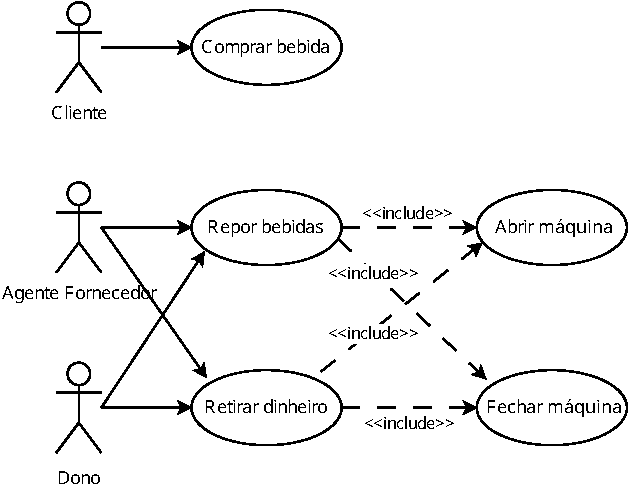
\includegraphics[width=0.58\textwidth]{imgs/UseCaseDiagramVendingMachine3.drawio.pdf}
          \caption{Possível solução apresentada de diagrama de casos de uso para o sistema de uma máquina de vendas}\label{fig:vending_machine}
      \end{figure}

      Foram ainda apresentados outros tipos de diagramas tipicamente usados no planeamento de aplicações, nomeadamente:
      \begin{itemize}
          \item \textbf{Diagrama de Estados (UML):} Descreve os diferentes estados que um objeto ou sistema pode assumir, destacando as transições entre esses estados e as ações associadas a cada um;
          
          \item \textbf{Diagrama de Sequências:} Modela a interação entre objetos num sistema em contexto temporal, exibindo a ordem das mensagens trocadas e facilitando a compreensão das dinâmicas do sistema;

          \item \textbf{Diagrama de Classes:} Um diagrama mais próximo da implementação, pois representa a estrutura do sistema orientado a objetos, mostrando classes, atributos, métodos e as relações entre as classes.
      \end{itemize}    

      Foram ainda cobertos os conceitos fundamentais de programação orientada a objetos bem como tópicos avançados como a manipulação de exceções, hierarquia, polimorfismo, e estruturas de dados. 

    \subsection{Formação de Excel}\label{subsec:excel}

      O Microsoft Excel é um programa da suíte Office 365 frequentemente utilizado para armazenar, organizar e manipular dados. É frequentemente utilizado em análise de dados ou criações de visualizações sendo muito usado no contexto da empresa, tornando a capacidade de o utilizar uma aptidão bastante favorável e procurada. 

      No entanto, esta formação acabou por tocar numa variedade de tópicos mais globais sobre boas práticas na empresa, tocando em tópicos como a forma de se apresentar e lidar com clientes, os cuidados a ter com a partilha de informação e o seu manuseamento, os cuidados a ter com a associação da marca da empresa às nossas vidas pessoais, pontualidade e mesmo a forma de resolver problemas e como a melhor contribuição para um projeto às vezes não precisa de ser técnica.

      Existem mais de 400 funções no Excel, permitindo uma interação entre dados bastante flexível, possibilitando a criação de cálculos e até gráficos e visualizações que normalmente não se associam a um programa de spreadsheets. Foram estudadas várias funções, desde a \texttt{SUM}, que simplesmente soma valores de duas células, até \texttt{VLOOKUP}, utilizada para procurar um valor específico na primeira coluna de um conjunto de dados e retornar o valor correspondente de uma coluna diferente na mesma linha. A seguinte lista não exaustiva contempla as funções estudadas durante o percurso:  

      \begin{itemize}
          \item \texttt{SUM}, \texttt{SUMIF}, \texttt{RANGE}, \texttt{CRITERIA}, \texttt{SUMIF}, \texttt{SUMIFS}, \texttt{COUNT}, \texttt{COUNTA}, \texttt{COUNTIF}, \texttt{AVERAGE}, \texttt{MAX}, \texttt{MIN}, \texttt{VLOOKUP}, \texttt{HLOOKUP}, \texttt{XLOOKUP}, \texttt{DCOUNT}, \texttt{DSUM}, \texttt{INDEX}, \texttt{ROUND}, \texttt{ROUNDUP}, \texttt{ROUNDDOWN}, \texttt{LEFT}, \texttt{RIGHT}, \texttt{MID}, \texttt{SEARCH}, \texttt{TRIM}, \texttt{IF}, \texttt{ISNA}, \texttt{MATCH}, \texttt{ISBLANK}, \texttt{ISERROR}.
      \end{itemize}    
    
    \subsection{Formação de SQL e Modelação}\label{subsec:sqlmodelacao}

      % podes ver a documentação deles para o debugger e tudo
      Dados estão em todo o tipo de aplicações, das pequenas às maiores, e estas aplicações usam bases de dados para guardar toda essa informação. A forma mais comum de guardar informação são bases de dados relacionais, constituídas por tabelas de dados que se podem relacionar entre si\cite{welcome-to-sql}. A linguagem mais amplamente usada para consultar estas bases de dados é SQL, sendo usada por uma variedade de serviços de gestão de bases de dados como Oracle, MySQL, PostgreSQL, Microsoft SQL Server\cite{sql-vs-mysql}.

      Durante a formação foram abordados todos os temas gerais da linguagem de gestão de dados, focando as seguintes características:

      \begin{itemize}
          \item \textbf{Pesquisas Básicas:} As pesquisas mais simples de SQL para obter dados das tabelas, utilizando o \texttt{SELECT}, \texttt{FROM} e \texttt{WHERE};
          
          \item \textbf{Ordenação e Agrupamento:} Usar cláusulas como \texttt{ORDER BY} e \texttt{GROUP BY} para organizar e agrupar os resultados de uma consulta SQL com base em critérios específicos;
          
          \item \textbf{Funções de Agregação:} Envolve o uso de funções como \texttt{SUM}, \texttt{AVG}, \texttt{MIN} e \texttt{MAX} para realizar cálculos em conjuntos de dados, geralmente em combinação com a cláusula \texttt{GROUP BY};
          
          \item \textbf{Junções (\textit{Joins}):} Usa-se para combinar duas ou mais tabelas usando as cláusulas \texttt{JOIN}, \texttt{INNER JOIN}, \texttt{LEFT JOIN}, \texttt{RIGHT JOIN} ou \texttt{FULL JOIN} e foram exemplificadas e visualizadas as diferenças entre cada caso;
          
          \item \textbf{Subconsultas:} Envolve o uso de consultas dentro de outras consultas, utilizando uma segunda cláusula \texttt{SELECT} na pesquisa;
          
          \item \textbf{Modificação de Dados:} Utilizou-se \texttt{INSERT}, \texttt{UPDATE}, \texttt{DELETE} e \texttt{COMMIT} para modificar e manipular os dados em tabelas específicas, ou seja, operações CRUD\footnote{CRUD (\textit{Create}, \textit{Read}, \textit{Update}, \textit{Delete}) é um acrónimo para formas de se interagir com informação guardada.}.
      \end{itemize}
    
    \subsection{Formação de Agile}\label{subsec:agilescrum}
    
      O Agile é uma abordagem de gestão de projetos e desenvolvimento com foco na flexibilidade, colaboração e satisfação do cliente. Distingue-se de outras abordagens pelo desenvolvimento iterativo, entrega incremental e capacidade de adaptação às mudanças.

      Este método diferencia-se do método tradicional Waterfall, linear com fases sequenciais, por ser iterativo. Enquanto uma abordagem Waterfall passará pelas fases de Especificação, Design, Desenvolvimento, Testes e Distribuição de forma sequencial sem avançar para um sem o último estar completo, a abordagem Agile passará por cada fase simultaneamente, entregando um resultado cada vez mais aprimorado no final de cada ciclo, como representado na Figura \ref{fig:agile-waterfall}.

      Foram transmitidos os princípios do manifesto Agile, os quais estão delineados na Tabela \ref{table:1}.

      \renewcommand{\arraystretch}{1.5}
      \begin{table}[htbp] % here top bottom page(a page just with images), ! would force it and could cause visual glitches, H is a better h that doesn't give problems by itslef (?)(https://tex.stackexchange.com/questions/132106/difference-between-h-and-h-in-float-position)
        \begin{tabularx}{\textwidth} { 
          >{\raggedright\arraybackslash}X 
          >{\raggedright\arraybackslash}X }
          
            %\hline
            \textbullet\ A nossa maior prioridade é satisfazer o cliente via a entrega contínua e antecipada do software. & \textbullet\ Aceitar mudanças nos requisitos, mesmo no final do desenvolvimento. Processos ágeis aproveitam  a flexibilidade das mudanças frequentes em prol vantagem competitiva do cliente. \\
            
            %\hline
            \textbullet\ Entregar software funcional frequentemente, de algumas semanas a alguns meses, com preferência no menor prazo. & \textbullet\ Pessoas de negócios e programadores devem trabalhar
            juntos diariamente ao longo do projeto. \\
            
            %\hline
            \textbullet\ Construir projetos com indivíduos motivados.
            Oferecer-lhes o ambiente e suporte necessários,
            e confiar neles para fazer um bom trabalho. & \textbullet\ O método mais eficiente e eficaz de transmitir informações para e entre uma equipa de desenvolvimento é a conversa presencial. \\
            
            %\hline
            \textbullet\ Em intervalos regulares, a equipa reflete sobre como se tornar mais eficaz, ajustando o seu comportamento. & \textbullet\ Processos ágeis promovem o desenvolvimento sustentável. Os patrocinadores, programadores e utilizadores devem ser capazes
            de manter um ritmo constante indefinidamente. \\
            
            %\hline
            \textbullet\ Atenção contínua à excelência técnica
            e bom design melhora a agilidade. & \textbullet\ Simplicidade --- a arte de maximizar a quantidade
            de trabalho não feito --- é essencial. \\
            
            %-
            
            %--

            %---

            %—

            %\textemdash
            
            %\hline
            \textbullet\ As melhores arquiteturas, requisitos e designs surgem de equipas organizadas por si mesmas. & \textbullet\ Software a funcionar é a principal medida de progresso.
        \end{tabularx}
        \caption{ \href{https://agilemanifesto.org/principles.html}{Princípios do manifesto Agile}}\label{table:1}
        \source{\cite{principios-agile-manifesto}}
      \end{table}

      O método ideal dependerá da do projeto, um método Waterfall é mais indicado para projetos menores e previsíveis, enquanto Agile é indicada para projetos mais avançados.

      \begin{figure}[H]
          \centering
          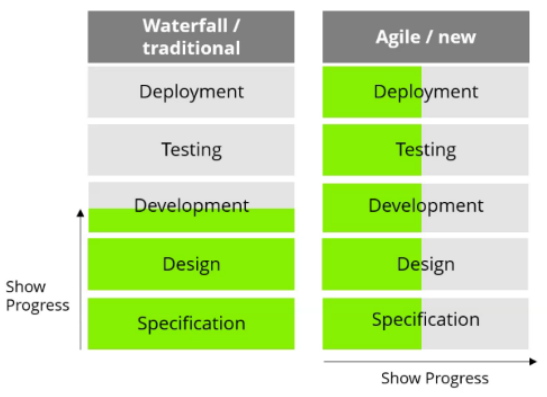
\includegraphics[scale=0.60]{imgs/agile-waterfall.png}
          \caption{Agile VS Waterfall}\label{fig:agile-waterfall}
          \source{Deloitte's Delivery Center}
      \end{figure}

    \subsubsection{Framework Scrum}\label{subsec:scrum}
    
      Scrum é um framework de Agile, especifica em detalhe como organizar o desenvolvimento, definindo papeis para as pessoas das equipas e descrevendo como aplicar o processo ágil, cuja representação gráfica apresenta-se na Figura \ref{fig:scrum}.

      \begin{figure}[H]
          \centering
          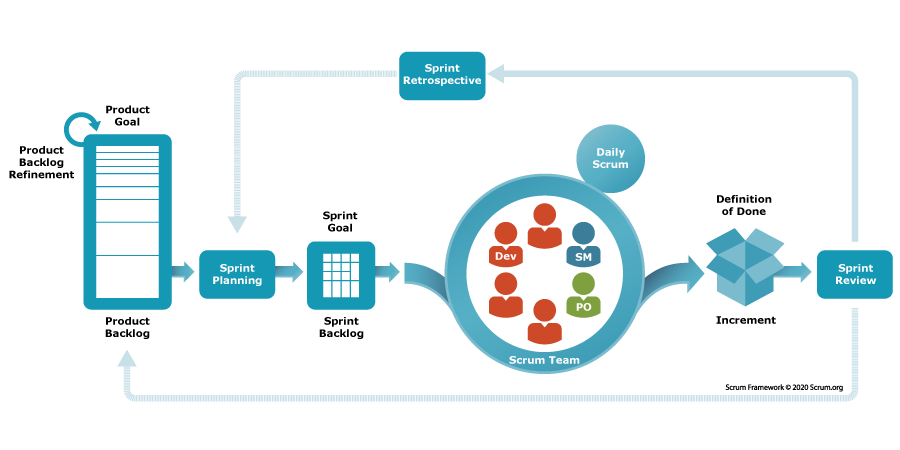
\includegraphics[scale=0.50]{imgs/scrum.png}
          \caption{\href{https://www.scrum.org/resources/what-scrum-module}{Scrum Process}}\label{fig:scrum}
          \source{\cite{scrum}}
      \end{figure}

      O Scrum requer um ambiente onde:
      \begin{itemize}
        \item Os Incrementos do trabalho são entregues em ciclos curtos de um mês ou menos, chamados \textit{sprints}. O feedback contínuo ocorre durante a \textit{sprint}, permitindo assim a inspeção e adaptação do processo e do que será entregue;
        \item A Equipa Scrum possui um \textit{Scrum Master}, um \textit{Product Owner} e Programadores, estes são responsáveis por transformar o trabalho planeado para a \textit{sprint} em algo apresentável;
        \item A Equipa Scrum e outros membros da organização, utilizadores e clientes conhecidos (\textit{stakeholders}), inspecionam os resultados da \textit{sprint} e ajustam devidamente o planeamento para a próxima.\cite{scrum}.
      \end{itemize}
    
    \subsection{Formação de OutSystems}\label{subsec:outsystems}

      OutSystems é uma plataforma \textit{low-code}\footnote{\textit{Low-code} é uma abordagem de desenvolvimento de software que minimiza a necessidade de programação manual, utilizando plataformas com interfaces gráficas e componentes reutilizáveis. Este método de desenvolvimento acelera o processo permitindo também a participação de profissionais menos experientes em programação.} para desenvolvimento, distribuição e manutenção de aplicações de forma eficiente. Com uma interface visual, como visível na Figura \ref{fig:interfaceoutsystems}, permite a criação de aplicações usando padrões bastante utilizados de forma rápida e eficaz, estando otimizado para a criação e a manutenção destas interfaces facilmente, não deixando de permitir a criação de interfaces e relações entre dados mais avançadas.

      \begin{figure}[H]
          \centering
          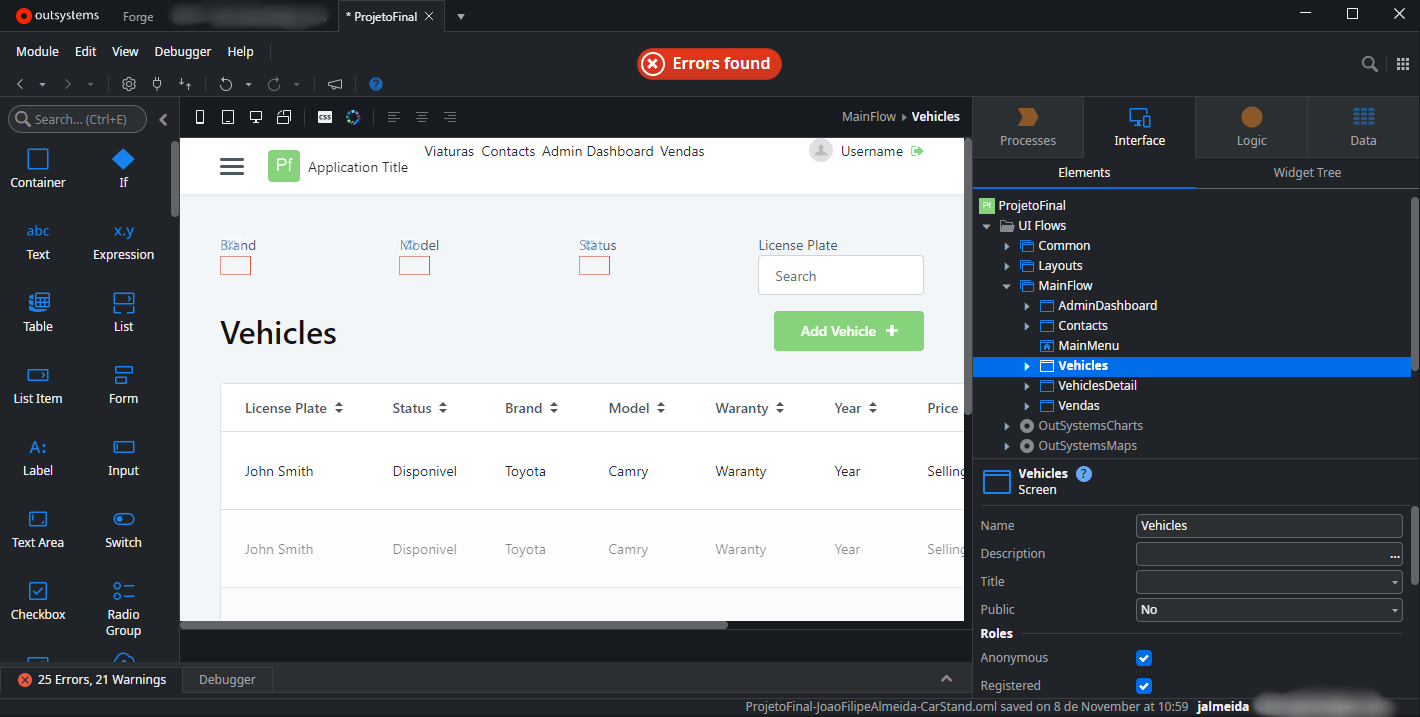
\includegraphics[width=\textwidth]{imgs/InterfaceOutSystems.png}
          \caption{Interface de OutSystems - Aplicação criada durante a formação}\label{fig:interfaceoutsystems}
          \source{Plataforma Interna da OutSystems}
      \end{figure}

      Para atingir o objetivo de ser uma plataforma visual que cubra o processo todo desde o desenvolvimento à publicação, OutSystems tem que oferecer um conjunto de ferramentas que se interliguem entre si, estas ferramentas são as seguintes:

      \begin{itemize} 
        \item \textbf{Ferramentas de Desenvolvimento:}
          \begin{itemize}
            \item \textbf{Service Studio:} Ambiente visual de desenvolvimento para aplicações Web e Mobile. Quando conectado pode publicar para o ``\textit{Platform Server}'' (servidores que compilam, publicam, gerem, executam e monitorizam aplicações.) Cada versão destas aplicações vai ser guardada na ``\textit{Platform Data Database}'';
            \item \textbf{Integration Studio:} Ambiente de desenvolvimento para criar extensões para a plataforma. Permite a criação de elementos dentro do Service Studio para interagir com recursos externos como código em C\# ou bases de dados.
          \end{itemize}
        \item \textbf{Ferramentas de Administração e Operação:}
          \begin{itemize}
            \item \textbf{Service Center:} Consola web de administração e gestão do servidor da plataforma. Inspecionar logs gerados pelo ambiente ou pelas aplicações, ou configurar definições do ambiente;
            \item \textbf{LifeTime:} Permite a gestão de todo o ciclo de vida da aplicação em vários ambientes, como, por exemplo, o ambiente de desenvolvimento, o ambiente de qualidade ou o ambiente de produção. É possível gerir as permissões de cada utilizador ou equipa, ver os ambientes e configurá-los ou a sua ordem no ciclo, analisar o desempenho das aplicações, ou efetuar \textit{deploys}\footnote{Passagem de código de um ambiente para outro de acordo com o \hyperref[fig:deployment-aggregator]{\textit{Deployment Agreaggator}}.} de código entre ambientes.
          \end{itemize}
        \item \textbf{OutSystems Forge:} Fonte de componentes para descarregar de forma a acelerar o desenvolvimento;
        \item \textbf{Comunidade:} Fóruns para troca de dicas, colocação de perguntas e obtenção de assistência\cite{outsystems-components-and-tools}.
      \end{itemize}

      Foram também explicados os conceitos mais importantes da plataforma, incluindo a aba da interface, a aba da lógica, a aba dos dados, aggregators, forms e validações, blocos e eventos, relações entre dados, \textit{roles}, Debugging. Para informação mais detalhada da plataforma, por favor refira à Secção \ref{sec:outsystems}.
    
    \subsection{Formação de Azure}\label{subsec:azure}

      A Azure é uma plataforma de computação da Microsoft, esta oferece uma panóplia de serviços Cloud para correr aplicações, servidores ou código na cloud.

      Existem três níveis distinguíveis de infraestrutura oferecidos: 
      \begin{itemize}
        \item \textbf{Infrastructure as a Service (IaaS):} IaaS é ideal quando o cliente quer manter controlo total sobre o sistema operativo e aplicações, trata-se de uma infraestrutura onde se virtualiza o hardware e o sistema operativo, deixando à responsabilidade do cliente manter o SO e as aplicações usadas atualizadas;
        \item \textbf{Platform as a Service (PaaS):} Em PaaS a plataforma de desenvolvimento e de publicação é fornecida, não é necessário gerir o sistema ou as aplicações subjacentes, mas o cliente mantém acesso ao código das aplicações que desenvolve, sendo oferecidas uma multitude de linguagens para as programar;
        \item \textbf{Software as a Service (SaaS):} Em SaaS a única responsabilidade do cliente é a gestão das contas e dos seus credenciais, SaaS refere-se ao fornecimento de aplicações já desenvolvidas para um cliente ou empresa como o Outlook ou o Office.
      \end{itemize}

      Dentro destes níveis de infraestrutura, a Microsoft disponibiliza uma variedade de serviços projetados para atender diversas necessidades, desde garantir a redundância de dados até facilitar a transferência de dados entre servidores locais, e a nuvem de Azure. Alguns destes serviços incluem:

      \begin{itemize}
          \item \textbf{Azure Blob Storage:}
          Armazenamento de objetos altamente escalável para dados não estruturados, como imagens e vídeos;
          
          \item \textbf{Azure Virtual Network:}
          Permite a criação de redes privadas na nuvem para conectar recursos Azure e estender a rede local;
          
          \item \textbf{Azure SQL Database:}
          Um serviço de bases de dados relacionais, proporcionando escalabilidade e segurança;
          
          \item \textbf{Azure ExpressRoute:}
          Estabelece conexões privadas e dedicadas à Azure, sem passar pela Internet, permitindo assim a transferência de dados rápida e seguramente;
          
          \item \textbf{Azure Backup:}
          Oferece soluções abrangentes de backup para proteger dados críticos, máquinas virtuais e aplicações;
          
          \item \textbf{Azure Logic Apps:}
          Permite a automação de fluxos de trabalho utilizando um designer visual permite a integração de serviços para criar aplicações poderosas;

          \item \textbf{Azure Cognitive Services:}
          Dezenas de serviços baseados em modelos de inteligência artificial oferecidos para integrar com as aplicações como por exemplo: Language cognitive, Speech cognitive, Vision cognitive, Decision cognitive.
      \end{itemize}

      Estes são apenas alguns exemplos dos infindáveis serviços disponíveis na plataforma Azure. Para informações mais detalhadas sobre a plataforma, por favor refira à Secção \ref{sec:plataforma-azure}.
      
    \subsection{Formação de OWASP}\label{subsec:owasp}

      A OWASP, ou \textit{Open Web Application Security Project}, é uma organização sem fins lucrativos dedicada a melhorar a segurança de software, especialmente no contexto de aplicações web. Foi fundada em 2001 e visa ajudar organizações a criar, desenvolver, obter, operar e manter aplicações que podem ser confiadas. \cite{about-the-OWASP-foundation}

      Uma das contribuições notáveis da OWASP é o \textbf{\textit{OWASP Top Ten}}. Esta é uma lista regularmente atualizada dos riscos de segurança mais críticos em aplicações web. A lista ajuda programadores, profissionais de segurança e organizações a priorizarem os seus esforços de forma a melhorar a segurança das aplicações web.
      
      As vulnerabilidades do \textit{OWASP Top ten} como especificadas em 2021 são as seguintes:

      \begin{itemize}
        \item \textbf{Controlo de Acesso Quebrado:} Problemas relacionados à má configuração ou implementação inadequada de controlos de acesso, permitindo a utilizadores não autorizados aceder a recursos protegidos;
      
        \item \textbf{Falhas Criptográficas:} Erros no uso de técnicas criptográficas, como encriptação e assinaturas digitais, que podem levar à exposição de dados sensíveis ou comprometer a segurança do sistema;
      
        \item \textbf{Injeção:} Vulnerabilidades que surgem quando dados não confiáveis são incorporados em comandos ou consultas, podendo levar à execução não autorizada de código;
      
        \item \textbf{Design Inseguro:} Riscos associados a falhas de design nas aplicações, refere-se aos riscos que não podem ser corrigidos com a implementação, salientando a importância de um planeamento adequado;
      
        \item \textbf{Configuração de Segurança:} Problemas decorrentes de configurações inadequadas ou em sintaxe errónea, especialmente em ambientes altamente configuráveis, que podem resultar em exposição não intencional de informações sensíveis;
      
        \item \textbf{Componentes Vulneráveis e Desatualizados:} Riscos relacionados ao uso de componentes (bibliotecas, frameworks) com vulnerabilidades conhecidas;
      
        \item \textbf{Falhas de Identificação e Autenticação:} Problemas de autenticação e identificação que podem permitir a utilizadores não autorizados aceder a contas protegidas ou obter privilégios indevidos;
      
        \item \textbf{Falhas de Integridade de Software e Dados:} Riscos associados a fazer suposições sobre integridade, especialmente relacionadas a atualizações de software e na utilização de extensões ou livrarias de terceiros;
      
        \item \textbf{Falhas de Registo e Monitorização de Segurança:} Desafios em garantir uma monitorização adequada e registo de eventos de segurança, o que pode afetar a visibilidade, alertas de incidentes e atividades de utilizadores;
      
        \item \textbf{Falsificação de Pedido do Lado do Servidor:} Situações em que um atacante pode induzir o servidor a fazer pedidos não autorizados em nome do utilizador\cite{OWASP-top-ten}.
      \end{itemize}

      Em suma, a OWASP é uma grande ajuda para qualquer empresa para manter um ambiente de aplicações seguras e confiáveis. A comunidade da OWASP é também bastante ativa e é ela que faz o projeto possível, contribuindo ativamente para identificar e documentar vulnerabilidades críticas.

    \subsection{Formação de MongoDB}\label{subsec:mongodb}

      O MongoDB é um sistema de gestão de bases de dados NoSQL amplamente utilizado, foi projetado para oferecer flexibilidade e escalabilidade em ambientes de desenvolvimento modernos. Ao contrário de Bases de Dados relacionais, o MongoDB adota uma abordagem baseada em documentos, armazenando dados em formato BSON (Binary JSON). A sua estrutura distribuída permite a manipulação eficiente de grandes volumes de dados, enquanto consultas mais complexas são facilitadas por índices e suporte a linguagens de consulta avançada. Além disso, o MongoDB oferece recursos de replicação para garantir alta disponibilidade e tolerância a falhas, sendo uma escolha popular para aplicações que requerem agilidade e desempenho em ambientes dinâmicos\cite{what-is-mongodb}.

      A plataforma usada para interação com estes dados através da nuvem é o Atlas, refira à Secção \ref{secsec:atlas} para mais informações sobre a plataforma.

    \subsection{Outras formações de curta duração}\label{subsec:outras-formacoes}

      De seguida apresento uma lista não exaustiva de outras formações de curta duração que muitas vezes se limitavam apenas a uma sessão ou reunião, este tipo de formações são frequentemente oferecidas sem caráter obrigatório aos empregados da empresa, e visam aprimorar as habilidades dos funcionários em diversas áreas, proporcionando-lhes uma vantagem competitiva, incentivando a versatilidade e ambientes em que os profissionais estão constantemente atualizados e no auge de sua eficiência:

    \begin{itemize}
      \item \textbf{Boas Práticas de Desenvolvimento:} Nesta formação foram abordados vários temas relacionados à criação de código legível e fácil de manter, foram abordados vários excertos analisados e simplificados colocando excertos relevantes em funções à parte, usando nomes de variáveis e funções descritivos, analisando a utilidade dos comentários, e analisando cada caso específico de forma a oferecer uma visão e capacidade geral de como fazer código profissionalmente;
      
      \item \textbf{Banca:} Focando-se no setor bancário, um setor onde se situam muitos dos clientes da companhia, foram estudados vários conceitos da área, e as formas como bancos se mantém rentáveis.
      Existem operações ativas, em que o banco se compromete a devolver o dinheiro ao cliente, como um depósito, é destas operações que o banco ganha o dinheiro que utiliza nas operações passivas, em que o cliente tem que pagar ao banco, por exemplo, um empréstimo, que terá juros;

      Foram analisados os riscos associados, incluindo: Risco de Conformidade, Risco Operacional, Risco de Sistemas de Informação, Risco de Estratégia, Risco Reputacional;
              
      \item \textbf{Seguros:} Focando-se no setor dos seguros, área também de muitos clientes da empresa, esta formação focou nos vários tipos de contratos que um individuo pode estabelecer com estas empresas e nas diferenças entre eles;
      
      \item \textbf{\textit{Getting Things Done}:} Esta formação veio a otimizar a gestão do tempo e aumentar a produtividade dos formados, proporcionando técnicas e ferramentas para a organização eficiente de tarefas pessoais e profissionais;
      
      \item \textbf{\textit{Capability Maturity Model Integration} (CMMI):} CMMI é um modelo que ajuda as organizações a otimizar a melhoria de processos e incentiva a comportamentos produtivos e eficientes que reduzem os riscos no desenvolvimento de software, produtos e serviços, definindo os seguintes níveis de maturidade: \textit{Initial}, \textit{Managed}, \textit{Defined}, \textit{Quantitatively Managed}, e \textit{Optimizing}\cite{cmmi}.

      %\item \textbf{Testes:} Abordando estratégias e práticas de teste de software, esta formação oferece conhecimentos sobre metodologias de teste, automação, e boas práticas para garantir a qualidade do software durante o ciclo de desenvolvimento.
    \end{itemize}


  \section{Conceitos Importantes}\label{sec:conceitos}

    Neste capítulo alguns conceitos importantes para compreender o projeto serão elaborados de forma a providenciar uma base forte para o resto do relatório. 

    \subsection{Mercado de Seguros de Londres}\label{sec:mercado-de-seguros-londres}

        Neste capítulo, far-se-á uma análise abrangente do mercado de seguros de Londres, de um ponto de vista histórico, contemporâneo e dos mecanismos intrínsecos que formam as seguradoras na capital britânica. Ao explorar a história e os funcionamentos do setor espera-se estabelecer as bases para uma análise detalhada do Projeto e como este se integra no mundo atual.

        \subsubsection{A evolução do setor de seguros de Londres}\label{secsec:a-evolucao-do-setor-de-seguros-de-londres}
    
            As origens do setor de seguros de Londres como o conhecemos hoje estendem-se por vários séculos, mas foi a partir do século \Romannum{17} com a fundação de Lloyd's e o grande fogo de Londres que se começou a formar o mercado de seguros como ainda hoje opera. 
        
            Antes deste século, um momento crítico na evolução do setor foi o caso de Gybbons v. Martin em 1537, onde o tribunal decidiu a favor do segurado em casos de ambiguidade do contrato. Aparentemente alguns \textit{underwriters} ou seguradores tinham concordado em fazer um seguro de vida para o Mr. Gybbons por um ano, e, com certeza, ele morreu uns dias antes do ano acabar. Mas os seguradores disseram que na verdade referiam-se a um ano lunar no contrato, que tinha acabado uns dias antes, claro que a Mme. Gybbons não aceitou e foi a tribunal que acabou por decidir em favor dela. 
            
            O caso estabeleceu o princípio de que qualquer incerteza na apólice seria resolvida a favor do segurado se fosse o segurador que redigisse o contrato. Esta decisão refletiu-se na indústria, causando uma solidificação do conhecimento do funcionamento e da regulação envolvendo estas matérias e contribuiu para a maturação do setor, sendo considerado um dos pilares na evolução sua evolução.  
        
            Em 1601, dois anos antes da morte da grande Rainha, um Ato do Parlamento visionava estabelecer um tribunal para ``ouvir e decidir causas decorrentes de apólices de seguro''. Embora o tribunal não fosse muito bem-sucedido, demonstrou que os princípios do seguro eram conhecidos entre aqueles que com eles lidavam.
            
            Edward Lloyd, nascido por volta de 1648, uma figura não diretamente envolvida em seguros, mas dono de uma cafetaria, desempenhou um papel fundamental no desenvolvimento do setor. Disponibilizou cabines na sua cafetaria para empresários dispostos a acartar uma parte do risco mediante uma taxa, e foi onde a tradição de '\textit{writing under}' começou. Os seguradores assinavam nas apólices debaixo do risco, surgindo assim o termo ``\textit{Underwriter}''.
        
            Em 1666, houve o Grande Incêndio de Londres, que devastou grande parte da cidade e consumindo inúmeras construções históricas, impulsionando mudanças no setor de seguros como a criação da primeira companhia de seguros de incêndio, The Sun. Isto incitou a mais movimento na cafetaria de Lloyd cujo negócio continuou a criar as bases para seguros marítimos e pagando quando necessário da parte dos seguradores como foi o caso, por exemplo, do naufrágio do Titanic\cite{lloyd-titanic}. A consistência de Lloyd's em pagar as perdas permanece consistente há mais de três séculos, sendo uma referência sólida na indústria de seguros\cite{lloyds-and-the-great-fire-of-london-propertycasualty360}.

        \subsubsection{O setor de seguros de Londres contemporâneo}\label{sec:o-setor-de-seguros-de-londres-contemporaneo}
    
            Em 2013, o setor de seguros representou impressionantes 20\% do Produto Interno Bruto (PIB) da cidade e 8\% do PIB de Londres. Esta significativa contribuição demonstra a importância económica do setor de seguros no contexto da capital britânica.
            
            Adicionalmente, o mercado londrino destaca-se ao segurar ativos valiosos e únicos. Exemplos notáveis incluem a cobertura para as pernas do renomeado jogador de futebol Cristiano Ronaldo e a voz única de Bruce Springsteen. Esta capacidade de segurar riscos especializados sublinha a flexibilidade e abrangência do mercado de seguros de Londres, atendendo às necessidades específicas de indivíduos e personalidades públicas.
        
            % 1 bilião deste lado do oceano é um milhão vezes um milhão
        
            % What Is an Insurance Premium? An insurance premium is the amount of money an individual or business pays for an insurance policy.
            % Gross written premium is a term that may refer to the total amount of premiums collected by an insurance company during a given period before any discounts or refunds are taken into account.
                
            Como visto na Figura \ref{fig:biggest-insurance-markets}, o mercado de seguros de Londres assume a primeira posição global, sendo o maior centro mundial de riscos comerciais e especializados. Em 2013, o mercado londrino controlou mais de £60 bilhões em ``GWP'', refere-se à quantidade de dinheiro paga à seguradora, fazendo deste o maior mercado mundial neste setor, superando significativamente a concorrência, com o segundo maior, o mercado de Bermuda, apresentando um tamanho de mercado de £25 bilhões em ``GWP''\cite{the-competitive-position-of-the-london-insurance-market,how-the-london-insurance-market-works}. % parencites
        
            \begin{figure}[H]
                \centering
                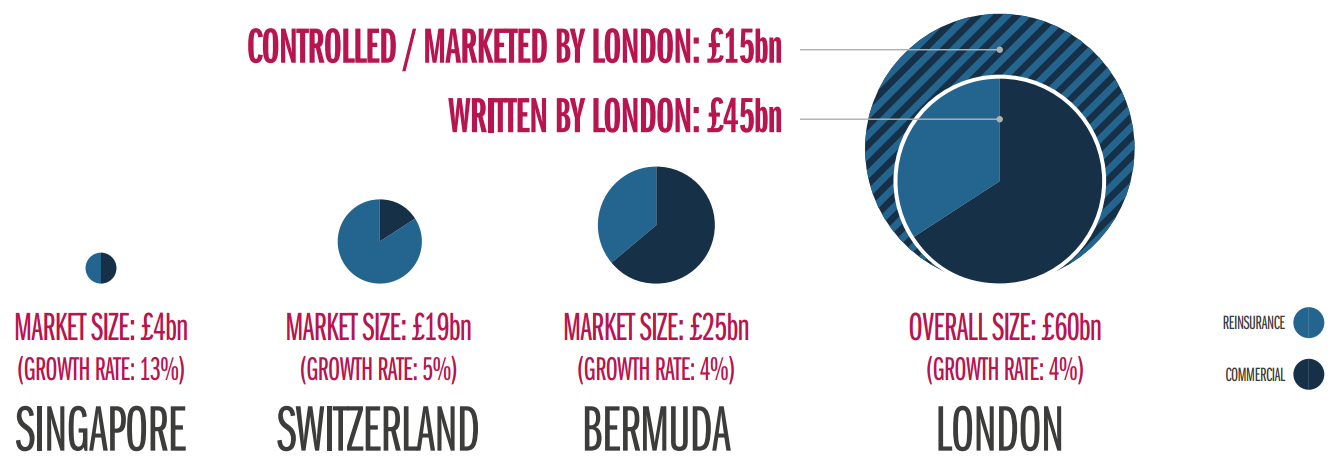
\includegraphics[width=\textwidth]{imgs/Biggest_Insurance_Markets.png}
                    \caption{Maiores mercados de seguros - 2013}\label{fig:biggest-insurance-markets}
                    \source{\cite{the-competitive-position-of-the-london-insurance-market}}
            \end{figure}

\begin{comment}
    %de acordo com https://lmg.london/wp-content/uploads/2019/07/London-Matters-CEO-Highlights-low-res.pdf
    Foi em 2013 20\% do GDP da cidade e 8% do GDP de Londres 
    segura cenas como as pernas do cristiano ronaldo, BRUCE SPRINGSTEEN'S VOICE.

    É o maior mercado, ``THE LONDON MARKET IS CURRENTLY THE LARGEST GLOBAL HUB FOR COMMERCIAL
    AND SPECIALTY RISK, CONTROLLING MORE THAN £60BN IN GWP IN 2013'', segundo ao de BERMUDA (ARKET SIZE: £25bn)

    (fogo de londres, llyods, marine insurance, de onde veio a palavra UNDERWRITER, etc)

    https://www.investopedia.com/ask/answers/051915/how-does-insurance-sector-work.asp
\end{comment}

        \subsubsection{Funcionamento e Terminologia de seguradoras}\label{secsec:mercado-de-londres-tradicional}

            O mercado de Londres é um campo onde jogam muitas empresas ou sindicatos que serão representadas pelos \textit{underwriters}. É normal subscreverem vários \textit{underwriters} para dividirem o risco entre si.

            O processo de emissão de seguros no século \Romannum{17} mantém-se no século \Romannum{21}: \\
            Aqueles que procuram segurar-se dirigem-se a um \textit{broker} e explicam o seu risco de forma detalhada, a qualidade e preço das ofertas depende da quantidade das informações fornecidas. O \textit{broker}, de seguida, vai ao encontro de \textit{underwriters} que representam um sindicato de um investidor, procurando os que podem oferecer melhores taxas consoante o risco em causa. O \textit{underwriter} pode dizer, por exemplo, ``Aceito 8\% a 2 por 250'', nesta situação este \textit{underwriter} cobre 8\% do risco, a uma taxa de 2 por 250 unidades monetárias. Desdobrando a proposta em mais detalhe:
            \begin{itemize}
                % \item Uma rate de 2 por 250
                \item Uma taxa de 2 por 250 indica que se o segurado tem 250€ de propriedade segurada exposta a risco, o segurado teria que pagar um prémio de 2€, ou seja, teria que pagar pelo seguro 2€ anualmente (ou mensalmente conforme estipulado). Mas isto apenas se estiver segurado a 100\%;
                \item Aceita 8\% do risco, ou seja, cobre apenas 8\% do valor caso o seguro se ative e recebe apenas 8\% do prémio.
            \end{itemize}
            De seguida o \textit{broker} dirigia-se a outros \textit{underwriters}, já com a taxa estipulada e tenta segurar o máximo de risco possível. Por vezes 100\% do risco é subscrito mas geralmente menos é segurado, e o proprietário ou comerciante é co-segurado para o resto, ou seja, é responsável pelo pagamento do restante\cite{rate-making,lloyds-and-the-great-fire-of-london-propertycasualty360}.

            % Titanic
            É frequente para projetos de alto capital serem segurados por bastantes \textit{underwriters} dividindo o risco entre eles, segundo os documentos de seguros do Titanic, por exemplo, o navio encontrava-se segurado por mais de 70 \textit{underwriters} diferentes\cite{titanic2,titanic}, como visto na Figura \ref{fig:titanic-placement-slip}.

            \begin{figure}[H]
                \centering
                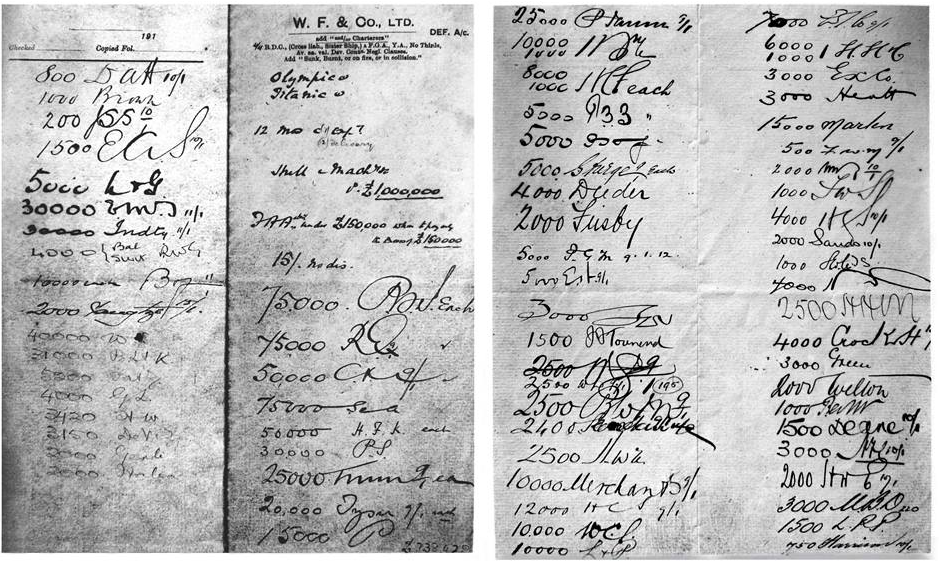
\includegraphics[width=\textwidth]{imgs/Titanic-Placement-Slip1.png}
                    \caption{Titanic Placement Slip — 2013}\label{fig:titanic-placement-slip}
                    \source{\cite{titanic}}
            \end{figure}

            % percebendo o que é "Aceito 8\% a 2 por 250"
            % https://www.businessinsider.com/personal-finance/what-is-underwriting
            % Underwriting helps set rates for loans, premiums for insurance policies, and the cost of risk in securities markets.

            % video que demonstra como underwriters são basicamente gajos que apostam no stock market: https://www.youtube.com/watch?v=QmJObCXq_Hk
        
            % https://www.irmi.com/term/insurance-definitions/placement-slips#:~:text=Placement%20slips%20are%20a%20general,transaction%E2%80%94not%20a%20binding%20contract.
            %Placement slips are a general understanding of the terms and conditions of a reinsurance transaction—not a binding contract.

            Com o processo geral estipulado pode-se agora detalhar as semânticas dos termos usados:

            \begin{itemize}
                \item \textbf{Underwriter:} O \textit{underwriter}, ou subscritor, é o profissional ou entidade responsável por assumir o risco do seguro. Avalia o risco, discute e estabelece os termos da cobertura e define a taxa e o prémio;
                
                \item \textbf{Broker:} O \textit{broker}, ou corretor, atua como intermediário entre o segurado e os \textit{underwriters}. Ele ajuda o segurado a compreender as suas necessidades, negocia com os \textit{underwriters} em nome dele e facilita o processo de subscrição;
                
                \item \textbf{Syndicate:} Um \textit{syndicate}, ou sindicato, refere-se a um grupo de \textit{underwriters} que se unem para assumir um determinado risco. Cada membro do sindicato contribui com uma parte da subscrição;
                
                \item \textbf{Placement Slip:} É um documento preliminar que resume os detalhes essenciais de um contrato de seguro. Inclui informações sobre o risco, cobertura, termos e \textit{underwriters} envolvidos;
                
                \item \textbf{Endorsements:} Referem-se a alterações feitas a uma apólice de seguro existente. Podem incluir a adição, remoção ou modificação de coberturas, condições ou termos do contrato. Estes são utilizados regularmente para ajustar a apólice conforme as necessidades do segurado;
    
                \item \textbf{Sign \& Close:} A etapa de ``Sign and Close'' refere-se ao processo de finalização de um contrato de seguro. Envolve a assinatura formal do contrato pelos participantes relevantes, confirmando a aceitação dos termos acordados. Este passo conclui o processo de subscrição e torna o contrato efetivo.

            \end{itemize}

            Este processo é comparável ao investimento numa empresa, \textit{underwriters} podem envolver-se com empresas de banca ou de seguros com títulos de valor variável de empresas (``\textit{securities}''). Da mesma forma que se pode lucrar ao investir num setor ou empresa, os \textit{underwriters} acartam risco para gerar lucro\cite{underwriting-insurance-loans-ipos-etc-explained-in-one-minute}.
    
            % To-Do: Podes falar de como funciona na plataforma:  Master facilities, placements, e a hierarquia de users e comapnhias etc

            \begin{comment}
                No âmbito dos seguros, o Tradicional Mercado de Seguros de Londres destaca-se como uma pedra angular na gestão de riscos, abrangendo uma rede complexa de profissionais que desempenham papéis vitais nos processos de subscrição, corretagem e seguradora. Para compreender a dinâmica deste mercado, é essencial aprofundar-se nas funções e interações de três intervenientes chave: Subscritores, Corretores e Seguradoras.

                (O que são insurers, brokers, underwriters, como funciona.)

                https://www.youtube.com/watch?v=e-sMZQB4XrQ
            v
                % in construction
                https://www.iii.org/publications/commercial-insurance/the-global-dimension/london-market

                The London Market is a distinct, separate part of the U.K. insurance and reinsurance industry centered in the City of London. Its main participants are insurance and reinsurance companies, Lloyd's of London syndicates, Marine Protection and Indemnity Clubs (P&I Clubs), and brokers who handle most of the business. The core of its activity is the conduct of internationally traded insurance and reinsurance business. This is mostly non-life insurance and reinsurance, particularly marine and aviation business, with an increasing emphasis on high-exposure risks.

                Lloyd’s of London is not an insurance company, but an insurance market of members, both corporate and individual. Lloyd’s members conduct their insurance business in syndicates, each of which is run by a managing agent. Over the course of its history, Lloyd’s has built a reputation for developing innovative coverages for the U.S. market including excess of loss reinsurance, kidnap and ransom insurance and more recently, terrorism insurance. Further information on Lloyd’s is available on its website at http://www.lloyds.com/
            \end{comment}

    \subsection{Desenvolvimento \textit{Low-Code}}\label{sec:low-code}

        Esta secção fornece uma resposta às questões de pesquisa sobre a definição do desenvolvimento \textit{low-code}, o seu ciclo de vida, bem como características e especificidades relacionadas.

        \subsubsection{Definição de Desenvolvimento \textit{Low-Code}}\label{secsec:defining_low-code}

            O termo ``\textit{low-code}'' surgiu em 2014 num artigo da \textit{Forrester Research} intitulado ``New Development Platforms Emerge For Customer-Facing Applications'' de Richardson C. \cite{bock2021lowcode,sanchis2020lowcode,bucaioni2022modelling,diruscio2022lowcode}, e desde a altura que tem ganhado tração e se solidificado como um campo da informática, num artigo de Alamin, \cite{alamin2021empirical} o desenvolvimento \textit{low-code} é definido como um paradigma que prioriza o mínimo de programação no processo, isto através de programação visual com interface gráfica e \textit{design} orientado por modelos. Noutras definições é também definido como um processo que envolve um esforço de programação mínimo com funcionalidades como \textit{drag-and-drop}\footnote{um paradigma de interface gráfica onde o utilizador pode selecionar elementos digitais, como ícones ou arquivos, movendo-os de um local para outro simplesmente ao clicar, manter o botão pressionado e soltando no destino desejado.} e desenvolvimento acessível a programadores não profissionais\cite{rokis2023exploring}.

        \subsubsection{Benefícios de Desenvolvimento \textit{Low-Code}}\label{secsec:beneficios_low-code}

            O desenvolvimento \textit{low-code} oferece diversas vantagens estratégicas, conforme destacado na lista abaixo. Ao acelerar o ciclo de desenvolvimento e envolver programadores menos especializados, esta abordagem responde eficientemente à escassez de profissionais especializados, permitindo uma entrega mais rápida de aplicações. A redução de custos é alcançada através da eficácia no desenvolvimento, otimização de recursos e diminuição dos custos de manutenção. Esta prática também aumenta a capacidade de resposta às exigências do mercado e dos negócios, adaptando-se rapidamente a situações dinâmicas e cumprindo prazos apertados, minimizando o esforço de manutenção e promovendo uma colaboração mais eficaz entre as equipas de desenvolvimento e as empresas, fomentando um ambiente propício à inovação digital\cite{rokis2023exploring,yan2021impacts}.

            \begin{itemize}
                \item \textbf{Aceleração do ciclo de desenvolvimento:} Aproveita as funcionalidades da plataforma, minimizando a programação manual e incorporando um desenvolvimento visual de aplicações;
                \item \textbf{Envolvimento de programadores cidadãos:} Aborda a escassez de programadores especializados, contribuindo para uma entrega mais rápida de aplicações;
                \item \textbf{Redução de custos:} Alcançada através da rapidez do desenvolvimento, utilização eficiente de recursos e diminuição dos custos de manutenção;
                \item \textbf{Aumento da capacidade de resposta às exigências do mercado e dos negócios:} Adapta-se rapidamente a situações dinâmicas e cumpre prazos apertados;
                \item \textbf{Diminuição do esforço de manutenção:} Minimiza erros e problemas relacionados à integração, permitindo a contínua manutenção menos exigente;
                \item \textbf{Melhor colaboração entre equipas de desenvolvimento e empresas:} Facilitada por modelos visuais e colaboração frequente ao longo do ciclo de desenvolvimento;
                \item \textbf{Promoção da inovação digital:} Fomenta uma cultura de aprendizagem e experimentação;
                \item \textbf{Mitigação dos riscos de \textit{shadow IT}\footnote{programas e sistemas de TI utilizados sem a aprovação do departamento de TI da organização, apresentando, portanto, riscos de segurança, integridade dos dados e outros.}:} Através de ferramentas administradas pela organização a profissionais não pertencentes à área 
                de TI, reduzindo soluções não autorizadas de TI e os riscos associados\cite{rokis2023exploring}.
            \end{itemize}

            Em 2019 a OutSystems analisou o estado da área de desenvolvimento \textit{low-code}, revelando as principais razões que impulsionam empresas a adotar estas metodologias como é possível observar na Figura \ref{fig:reasons_to_use_low-code}, estas incluem: a aceleração da inovação e transformação digital, o aumento da capacidade de resposta às exigências do negócio, a redução da dependência de habilidades técnicas de difícil contratação, a mitigação de despesas devido a tecnologias obsoletas, a proteção contra a rápida evolução tecnológica, e permitir programadores cidadãos aprimorarem processos internos.
    
            \begin{figure}[htbp]
                \centering
                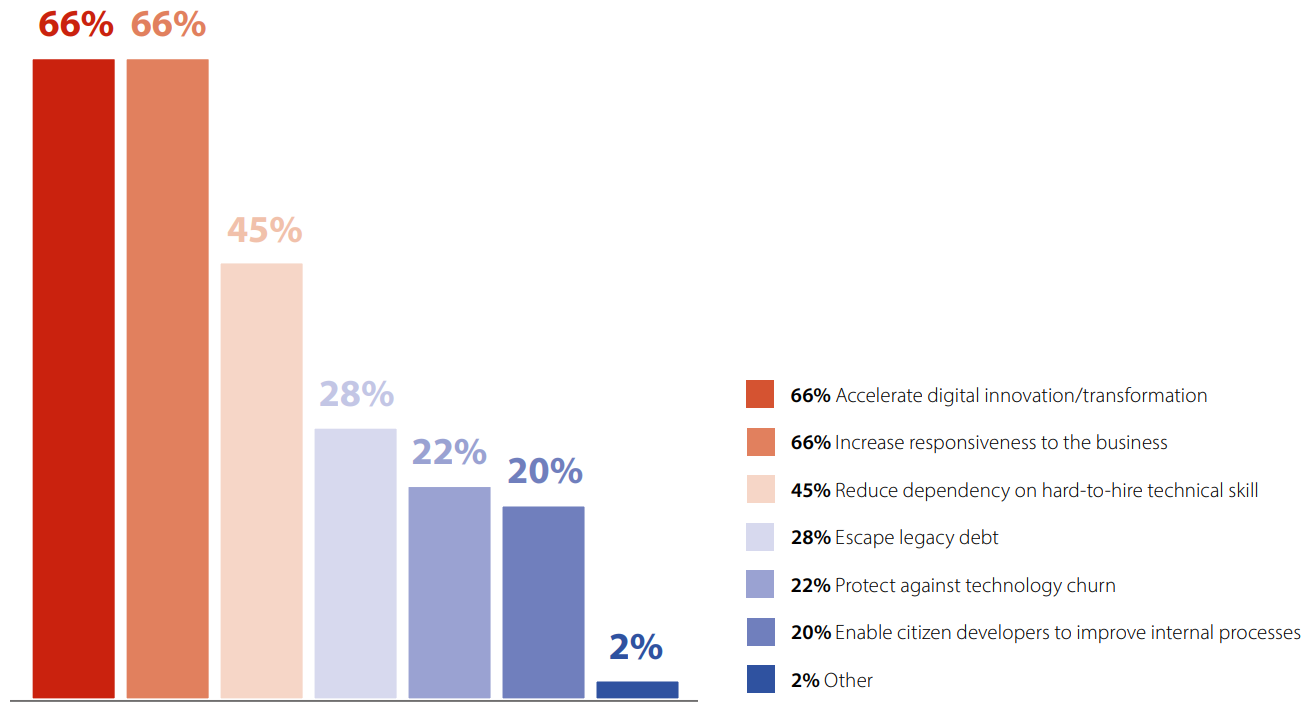
\includegraphics[width=\textwidth]{imgs/reasons_to_use_low-code.png}
                    \caption{Maiores razões para usar \textit{low-code}}\label{fig:reasons_to_use_low-code}
                    \source{\cite{state-of-lowcode-outsystems}}
            \end{figure}

        \subsubsection{Limitações de Desenvolvimento \textit{Low-Code}}\label{secsec:limitacoes_low-code}

            A OutSystems identificou no seu estudo ``The State of Application Development'' de 2019, segundo os participantes os três desafios que mais dificultam a entrega de aplicações móveis e de web são:
            \begin{itemize}
                \item Integração com sistemas obsoletos ou ultrapassados;
                \item Requerimentos não bem definidos e inconstantes;
                \item Tempo necessário para testar.
            \end{itemize}
                
            Identificando também as maiores causas de retardam a entrega destas aplicações, como visto na Figura \ref{fig:atraso_app_low_code}, sendo estas, a Integração de sistemas legados/APIs ausentes ou que necessitam de melhorias, Requisitos difusos/em constante mudança, Testes/Garantia de Qualidade, Proteção e teste de penetração em segurança, Preocupações com privacidade de dados, Falta de habilidades técnicas de desenvolvimento, \textit{Design} UX/UI (incluindo \textit{design} responsivo), Implantação/coordenação com operações de TI\cite{state-of-lowcode-outsystems}.
                
            \begin{figure}[htbp]
                \centering
                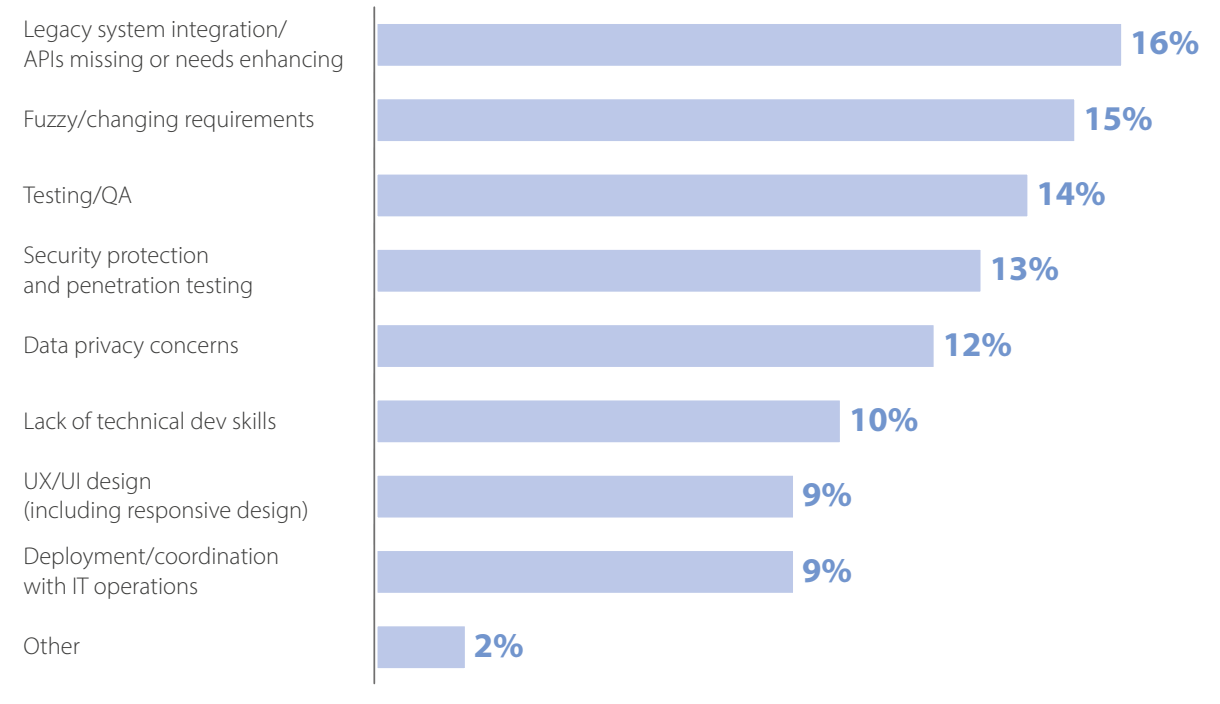
\includegraphics[width=\textwidth]{imgs/causas_espera_na_entrega_aplicacoes_low_code.png}
                    \caption{Maiores causas de atrasos na entrega de aplicações \textit{low-code}}\label{fig:atraso_app_low_code}
                    \source{\cite{state-of-lowcode-outsystems}}
            \end{figure}
            
            Segundo o artigo ``The Impacts of Low/No-Code Development on Digital Transformation and Software Development'' do autor Zhaohang Yan podem ser identificadas estas limitações no método:

            \begin{enumerate}
                \item \textbf{Limitação na Customização/Flexibilidade:}  Estas plataformas têm pré-implementações fixas em muitas áreas e casos, tornando-as menos customizáveis sacrificando flexibilidade. Programar funcionalidades customizáveis específicas é uma opção, mas pode ser difícil e moroso, podendo não ser o método ideal para aplicações que precisem de ser altamente customizáveis com um nível de complexidade mais elevado.
            
                \item \textbf{Limitação na Scalabilidade:} Muitas destas plataformas focam num processo célere na produção e entrega de aplicações de pequena a média escala, sendo uma ferramenta menos testada para aplicações de grande escala.
            
                \item \textbf{Preocupações de Segurança:} A utilização de plataformas \textit{low-code} implica a inteira dependência da segurança da plataforma em uso. Organizações dependentes destas plataformas enfrentam riscos, uma vez que a segurança dos dados não está totalmente sob o seu controle. Se, por exemplo, os fornecedores da plataforma encerrarem as operações, as atualizações de segurança contínuas tornam-se incertas, deixando as organizações incapazes de lidar com novas vulnerabilidades.

                \item \textbf{\textit{Vendor lock-in}:} Refere-se à dependência de um cliente em relação a um fornecedor, e à sua capacidade de mudar para outro. No contexto das plataformas \textit{low-code}, à medida que investem mais num fornecedor específico, o processo de mudança torna-se mais dispendioso e complexo e difícil\cite{yan2021impacts}.
            \end{enumerate} 

            Em suma, existem vários detalhes específicos ao desenvolvimento \textit{low-code}, sendo importante analisar as vantagens expostas e as desvantagens identificadas e os seus pesos na implementação num dado projeto.

        \begin{comment}
Here are a couple of good academic articles you can look into for learning about low-code programming:

1. Exploring Low-Code Development: A Comprehensive Literature Review

Authors: Fábio S. O. Ramos, Daniel L. M. Batista, Marco Túlio P. Viana, and Cláudia M. S. Fernandes
Published in: (2020) Proceedings of the 54th Hawaii International Conference on System Sciences (https://www.researchgate.net/publication/375218739_Exploring_Low-Code_Development_A_Comprehensive_Literature_Review)
This article provides a comprehensive overview of low-code development (LCD). It delves into the key concepts, benefits, limitations, existing research, and future directions for LCD.

2. The Impacts of Low/No-Code Development on Digital Transformation and Software Development

Author: Zhaohang Yan
Published in: (2023) Informatics, 10(2), 22 (https://www.researchgate.net/publication/357417399_The_Impacts_of_LowNo-Code_Development_on_Digital_Transformation_and_Software_Development)
This article focuses on the impact of low-code/no-code (LCNC) development on digital transformation and software development. It explores the advantages and disadvantages of LCNC platforms and how they can accelerate software development and contribute to digital transformation initiatives.

These are two well-regarded articles that offer a good starting point for understanding low-code programming from an academic perspective. They provide a solid foundation for further research or exploration of the topic.

Here are some additional tips for finding good academic articles:

Search academic databases: Use databases like Google Scholar, ScienceDirect, or JSTOR to search for articles by title, author, or keywords. You can also filter your search by publication date or peer-reviewed status.
Look for articles in reputable journals: Top academic journals in computer science and information technology often publish articles on emerging technologies like low-code development.
Check the references section of existing articles: Once you find a good article, look at the references section to discover other relevant academic works on the topic.
        \end{comment}

    \subsection{Terminologia do Projeto}\label{sec:terminologia_do_projeto}
        
        Existem vários conceitos que serão frequentemente utilizados ao longo deste relatório e são frequentemente usados no contexto de trabalho, esta secção servirá para estabelecer bem os seguintes conceitos:

        \begin{itemize}
            \item \textbf{User Stories:} As \textit{User Stories} (Histórias de Utilizador) são descrições detalhadas de funcionalidades do sistema, frequentemente utilizadas para comunicação entre os interessados e para orientar o desenvolvimento de software. Elas são a base para o desenvolvimento na plataforma;

            \item \textbf{Defects}\label{bulletlist:defects}: Uma incongruência identificada entre o funcionamento do programa e as USs (User Stories) definidas. São identificados com uma prioridade e registadas na Jira como descrito na Secção \ref{secsec:jira};
            
            \item \textbf{Incidentes}\label{bulletlist:incidentes}: Problemas submetidos por utilizadores da aplicação através da plataforma ServiceNow [\ref{sec:service-now}], o utilizador pode marcar a submissão de duas formas:
            \begin{itemize}
                \item \textbf{Request}: O utilizador coloca esta \textit{label} quando não tem a certeza se o problema está na forma de utilização ou de facto na plataforma;
                \item \textbf{Incidente}: Se o utilizador está confiante que o problema com que se depara é de facto um problema da plataforma, marca desta forma.
            \end{itemize}
                
            
            \begin{comment}
                Passa para a triagem como forma de request ou incidente (request - quando o user está na duvida se é problema dele ou se é a plataforma que bugou, se é erro mesmo, converte-se em incidente.) - temos SLA(pesquisa, é termo informatico, é o termo que contratualizamos com a RIL para dar suporte, não pode demorar tipo 3 meses)- o team leader apanha o incidente e dá prioridade low median high ou critical e manda mensagem ao user a dizer que desculpe e que estamos a ver (por exemplo erro de formatação é low, erro 502 é critical). Não há uma regra especifica, se tá lá um medium à uma semana pode ser que se pegue.
Backlog - vai dando incidentes
            \end{comment}

            \item \textbf{GAP}: Caso específico em que a implementação está de acordo com a \textit{user story}, mas a esta não contempla uma situação que se precisava de ter em conta.
            
            Por exemplo: Se a \textit{user story} for ``Efetuar um programa que conte de um a cinco'', e o programa conte da seguinte forma: ``1, 2, 3, 4, 5'', mas se descubra através de testes ou interações com utilizadores e confirmando com um BA ou alguém mais acima na hierarquia que esteja familiarizado com o que a aplicação tem que fazer, que a aplicação teria que contar também decimais desta forma: ``1.1, 1.2, 1.3...'', então, como não estava bem explícito na US, considera-se um GAP.
            
            É por isso que antes de reportar um novo \textit{defect}, é geralmente necessário confirmar que o comportamento que acontece não está contemplado numa \textit{user story}, porque se estiver, será um GAP. Neste caso a \textit{user story} terá que ser revista, e a empresa cliente terá possivelmente que pagar por outra US, visto que o pagamento se faz por USs;
            
            %GAP - Quando falta alguma coisa na user storie e se reflete no desenvolvimento
            %- Por exemplo, caso especifico em que UW não recebia notificação, mas aquele.
            \item \textbf{Stamps:} Num contexto de lógica de seguradoras, os Stamps representam a aprovação formal de um \textit{underwriter} para assumir um risco específico. Cada \textit{underwriters} coloca seu carimbo no \textit{Placement Slip} como uma indicação da sua subscrição no risco.

            No contexto da plataforma, stamps são carimbos associados a uma organização cujos UWs pertencentes podem usar. Após a definição dos detalhes de um contrato e antes do envio da submissão aos UWs pertencentes, são atribuídos \textit{roles}, estes \textit{roles} são escolhidos consoante o stamp de cada UW. Podendo um UW não ter nenhum \textit{role};
                
            % todo confirmar que é isso que quer dizer, e mudar também nas abreviações e noutro sítio se for pra mudar
            \item \textbf{Mutual Responsibility Contract(MRC):} O MRC, é um documento obrigatório a todos os contratos na plataforma que contém detalhes sobre o acordo que possam não estar contemplados na plataforma como informações de cobertura de uma apólice de seguro ou detalhes sobre o risco coberto, ou as condições e termos do contrato;

            \item \textbf{Endorsements:} Como explicado na Secção \ref{secsec:mercado-de-londres-tradicional}, referem-se a alterações feitas a um contrato, na plataforma existem os seguintes tipos de endorsement:
            \begin{enumerate}
                \item Annual Resigning Statement;
                \item Cancellation;
                \item Decrease Cover;
                \item Increase Cover;
                \item Mid-Term Broker Change;
                \item Other Change to Cover;
                \item Reinstatement Provision;
                \item Tax Schedule;
                \item Mid Term Market Change (o único \textit{endorsement} que requer um \textit{Sign \& Close}).
            \end{enumerate}
            A termos de lógica de negócio a única diferença está entre o Mid Term Market Change e os restantes, devido ao seu requisito de ser feito num contrato \textit{Signed and Closed};

            \item \textbf{Corrections:} Correções são modificações realizadas para retificar erros ou informações incorretas em documentos relacionados ao seguro. Estas podem incluir ajustes nas apólices, documentos contratuais ou registos relacionados à subscrição. Na plataforma existem três tipos de \textit{corrections}:
            \begin{itemize}

                 \item \textbf{Cancel Contract:}
                 A ação ``Cancel Contract'' permite ao \textit{broker} cancelar completamente um \textit{placement} de forma irreversível. A aceitação por parte da seguradora de um pedido de cancelamento reduz a linha escrita para zero e altera o estado do contrato para Cancelado. Uma vez concluído o cancelamento, é possível reutilizar o UMR. 
                 
                 No caso de cancelamento de uma \textit{master facility}, as partes não acordadas serão canceladas assim que o líder da \textit{facility} aceitar o cancelamento. Um pedido de cancelamento para qualquer \textit{declaration} já vinculada que utilize a \textit{facility} será acionado simultaneamente;
                 
                 \item \textbf{Cancel and Replace:}
                 A ação ``Cancel and Replace'' está disponível ao longo do processo de \textit{Firm Order}. Permite ao \textit{broker} substituir um contrato cancelando o original simultaneamente de forma irreversível. A aceitação por parte da seguradora de uma ressubmissão vincula a linha escrita ao novo contrato, reduzindo a linha no contrato anterior para zero e alterando o estado para Cancelado. Não é possível assinar e fechar até que todas as submissões originais sejam canceladas e todas as ressubmissões sejam aceites;
                 
                 \item \textbf{Panel Change:}
                 A ação ``Panel Change'' está disponível ao longo do processo de \textit{Firm Order}. Permite ao \textit{broker} fazer alterações nos detalhes da linha dos participantes no contrato. Incluindo em painéis de \textit{facilities}, desde que o líder da \textit{facility} não seja um Slip, Lloyds, XIS ou LIC Lead no \textit{placement}. Detalhes da linha que podem ser alterados incluem linha escrita e stamp. A ação é irreversível, sendo necessário responder a todos os pedidos de ``Panel Change'' antes de assinar e fechar.
            \end{itemize}           
            % info disto acima:
            \begin{comment} 
            1. Cancel Contract
ssions set by your Organisation.
Cancel Contract allows the Broker to cancel the placement in its entirety.
This action is irreversible.
A Carrier’s acceptance of a Cancellation Request reduces the written line to zero and changes the status of the Contract to Cancelled.
Once the cancellation is complete and closed it is possible to re-use the UMR.

Facility Panel Cancelation:
Non-agreement parties on a Facility panel will be cancelled once the Facility Leader accepts the cancellation.
A Cancellation Request for a bound Declaration Agreement Party will be triggered simultaneously.
Pending Agreement Parties will be withdrawn, conditionally offers rejected and then removed.

2. Cancel & Replace
The Cancel & Replace action is available throughout the Firm Order process, subject to configurable permissions set by your Organisation.
Cancel and Replace allows the Broker to replace the Contract whilst cancelling the original simultaneously.
This action is irreversible.
A Carrier’s acceptance of a resubmission binds the written line to the new Contract whilst reducing the line on the previous Contract to zero and changing the status to Cancelled.
Validation will prevent a Carrier providing a mixed response on a Sectioned Resubmission. All Sections must be either all accepted or all rejected.
It is not possible to Sign and Close until all original submissions are cancelled and all Resubmissions are accepted.

Facility Panel C&R:
Non-agreement parties on a Facility panel will be bound on the new Contract and cancelled on the previous contract once the Facility Leader accepts the resubmission.

Endorsements:
Endorsements created from a Contract version will be linked with the associated Contract and remain with that version. Once the Cancel and Replace action is triggered, any new Endorsements will attach to the new version of the Contract.

3. Panel Change
The Panel Change action is available throughout the Firm Order process, subject to configurable permissions set by your Organisation.
Panel Change allows the Broker to make amendments to the line details of following participants to the Contract with effect from the inception of the contract.
This includes Facility panels, provided that the Facility Leader is not a Slip, Lloyds, XIS or LIC Lead on the Placement.
Line details that can be amended are written line and stamp. Panel Change cannot be used to change contractual roles.
This action is irreversible.
It is not possible to Sign and Close until all Panel Change requests have been responded to.

Facility Panels:
The use of Panel Change is generally not suitable if you need to modify the participation role of a member of a Facility panel. The C&R function is suggested.
A Facility Leader with a following market must be cancelled prior to modifying their role on a Resubmission.
A Declaration Agreement Party must be cancelled prior to modifying their role on a Resubmission.
A Follower must be cancelled by the Facility Leader prior to promoting their role to an Agreement Party.
In these scenarios, Cancel Line, Cancel Contract or C&R may be a more suitable alternative.

4. Cancel Line (available at individual carrier line level)
The Cancel Line action is available up until Sign and Close for following markets only.
This includes Facility panels, provided that the Facility Leader is not a Slip, Lloyds, XIS or LIC Lead on the Placement.
Should you need to cancel a Lead line, it will be necessary to cancel the Placement in full.
A Carrier’s acceptance of a Cancellation Request reduces the written line to zero and removes the line from the Contract.

Cancelling a Facility Panel line:
Non-agreement parties on a Facility panel will be cancelled once the Facility Leader accepts the Facility line Cancellation Request.
Bound Declaration Agreement Parties are selected automatically for cancellation when the Broker triggers a Facility line Cancellation Request for a Facility Leader
Pending Declaration Agreement Parties must be withdrawn to proceed.
A Cancel line request for a bound Declaration Agreement Party can be selected independently in isolation.
This action can be withdrawn if the Cancel line request is pending.
            \end{comment} 

            \item \textbf{Master Facilities:} Master Facilities ou Facilities referem-se a um conjunto de seguradoras que se juntaram e aceitaram fazer parte da \textit{facility}, esta que depois pode ser adicionada como painel conjunto a um contrato;

            \item \textbf{Declarations e Open Market Contracts:} \textit{Declarations} e contratos de mercado aberto referem-se a contratos que utilizam painéis de \textit{facilities} ou não. As \textit{declarations} são contratos que envolvem uma ou mais \textit{facilities}, já contratos de mercado aberto envolvem apenas UW individuais;
            
            \item \textbf{Off-platform Underwriters:} \textit{Underwriters} fora da plataforma são profissionais que assumem riscos de seguro, mas que não utilizam diretamente a plataforma para a subscrição. A interação eficaz com esses \textit{underwriters} é simulada na plataforma por um UW \textit{off-platform} cujas respostas ao contrato são controladas pelo \textit{broker}, desta forma este deve alinhar com estes UWs fora da plataforma e consoante o decidido, colocar a resposta por eles na plataforma;
            
            \item \textbf{Archive Placements:} Refere-se ao armazenamento organizado de registos e documentos relacionados a colocações de seguros já fechados. É muito usado na transferência de dados de uma plataforma antiga;
            
            \item \textbf{Placements:} Referem-se a uma estrutura que pode conter vários contratos. É obrigatório um contrato se encontrar sempre dentro de um \textit{placement};
            
            \item \textbf{Firm Order:} É o processo vinculativo executado pelo \textit{broker} que manda os pedidos de aceitação do cancelamento ou do endorsement ou das linhas do contrato para os UWs. Pelo que mandar uma \textit{firm order} será mandar o pedido em contexto para os UWs apropriados;
            
            \item \textbf{Retrofit:} É a passagem de código de um ambiente mais avançado, ou seja, mais próximo do ambiente de produção, para um ambiente de mais baixo nível, como por exemplo um dos ambientes de desenvolvimento, isto pode ser necessário, por exemplo, se um \textit{defect} teve que ser resolvido num ambiente mais alto de forma a que a sua resolução chegue mais rápidamente a produção, neste caso ter-se-ía que trazer este código para os ambientes mais baixos também, a este processo chama-se retrofit, refira à Secção \ref{secsec:versionamento} para mais informação sobre ambientes;
            
            \item \textbf{Cancel Line:} Cancelar uma linha representa a anulação de uma linha específica num contrato de seguro, ou seja de um UW ou de uma \textit{facility}. Após os relevantes terem aceite, se não tiverem nenhum \textit{role} gerado pelos seus stamps, o \textit{broker} pode lhes fazer um cancel line, que irá mandar um pedido para se retirarem;
            
            \item \textbf{Withdraw:} A ação de withdraw está disponível depois de fazer uma submissão para um UW, mas antes deste aceitar. Ao fazer \textit{withdraw}, o UW não poderá mais aceitar o pedido;

            \item \textbf{Business Analysts (BA)}: Os \textit{Business Analysts} analisam e compreendem os processos e funcionamento de negócios, identificando oportunidades de melhoria, desempenhando tarefas como análise de dados, comunicação com clientes, documentação de processos, testes e validações. 

            Na prática, os BA's são generalistas da equipa que têm uma boa noção de como a aplicação se deve comportar e a quem se recorre em caso de dúvida.
           
        \end{itemize}

  \section{Organização do Projeto e Empresa}\label{sec:org-projeto-empresa}

    Nesta secção será explorada a estrutura e organização da Deloitte e do projeto no que toca a recursos humanos, licenças, programas, e a integração com os restantes mecanismos de gestão da Deloitte PT. Devido à grande escala do projeto RIL este envolve uma colaboração extensa entre a Deloitte PT, a Deloitte UK e a Deloitte India. 

    \subsection{Estrutura Organizacional da Deloitte PT}

        \begin{comment}
            
        Falar das formações, como são usadas para pôr os novos contratados a par com o resto da equipa e como forma de ver em que projeto é que ficariam melhor

        explicar a hierarquia de intern, brightstart, para junior developer, para developer, para team leader, para etc. deloitte

        explicar os buddys

        explicar os carrear coaches, como podem ser mudados todos os anos e como temos reuniões mensais com eles sobre perguntas de carreira na deloitte ou outros temas que possamos não nos sentir confortaveis a falar com o nosso team leader
        \end{comment}
        
        A Deloitte Portugal organiza-se de forma a proporcionar uma integração eficiente dos novos contratados, facilitando o seu desenvolvimento de carreira e apoio contínuo aos colaboradores. Nesta secção, abordaremos as principais práticas e elementos relacionados à estrutura organizacional da Deloitte PT.
        
        \subsubsection{Formações e Integração}\label{formacoes_e_integracao}
        
            As formações, como já falado no primeiro capítulo, desempenham um papel crucial na integração de novos colaboradores à equipa em que são inseridos enquanto elevam simultaneamente  as capacidades dos novos recrutados a termos de ferramentas que são frequentemente usadas na empresa ou em projetos da empresa. Servem também como uma avaliação inicial das aptidões de cada ``new hire'' para mais facilmente identificar um projeto que se adeque a ele.
        
        \subsubsection{Hierarquia e Progressão de Carreira}

            Cada profissional tem um estatuto para com a hierarquia da empresa. Esta hierarquia dita quem tem poder de decisão sobre quem, quem é que faz os ``check-ins'', e reflete-se também no salário de cada um.

            \textbf{Check-Ins}: Os ``check-ins'' são reuniões mensais realizadas entre cada membro da Deloitte e o seu superior. Durante estas reuniões, são avaliados pontos fortes e fracos desde o último encontro, identificam-se áreas de melhoria e é dada uma nota. Estes encontros são essenciais para manter o desenvolvimento profissional positivo e saber quais são os pontos de melhoria dos profissionais, permitindo um contínuo aprimoramento das suas habilidades. São também estabelecidas metas, objetivos anuais ou mensais.
                        
            Existem vários estatutos hierárquicos, por ordem crescente de hierarquia, os seguintes:

            \begin{itemize}
                \item \textbf{Trainee} \\
                    Um estatuto inicial na Deloitte, reservado para aqueles que estão nos primeiros etapas de suas carreiras. Os trainees geralmente estão a ter a sua primeira experiência de trabalho na área ou estão a trabalhar no contexto de um estágio curricular ou profissional e estão em processo de aprendizagem e desenvolvimento;
                \item \textbf{Programmer} \\
                    A designação para quem foi contratado como programador e tenha pouca experiência, e um a dois anos;
                \item \textbf{Experienced Programmer} \\
                    Após algum tempo e feedback positivo, os Programmers são promovidos ao estatuto de Experienced Programmers;
                \item \textbf{Team Leader} \\
                    O estatuto de Team Leader é alcançado por indivíduos que estão na empresa há algum tempo e demonstraram já capacidade de liderança e tenham uma boa ideia dos funcionamentos internos da empresa. Nesta posição, assumem a responsabilidade por uma equipa, estando encarregados de realizar os Check-ins com os restantes membros.
                    
                    Podem também, a partir deste título, assumir o papel de ``Career Coach'' para outros membros da empresa;
                \item \textbf{Pro Manager} \\
                    Enquanto os papéis anteriores necessitavam ainda de um grande contacto com o projeto e as tarefas em si, os seguintes são papéis que envolvem maioritariamente gestão de recursos.
                    
                    Têm um papel-chave na gestão de equipas e projetos;
                \item \textbf{Manager} \\
                    Uma posição de gestão mais avançada, envolvendo mais responsabilidades significativas na coordenação e supervisão de projetos;
                \item \textbf{Senior Manager} \\
                    O último nível a que se pode ser promovido dentro da categoria de gestão com mais poder e responsabilidade na liderança estratégica dos projetos e gestão do cliente;

                \item \textbf{Associate Partner} \\
                    Uma posição associada já à gestão de colaborações da Deloitte, começam a ter responsabilidades em relação aos novos contratados e a que projetos é que são alocados, bem como o contacto e fecho de contratos com empresas parceiras;
                \item \textbf{Partner} \\
                    O estatuto mais elevado, com acrescidas responsabilidades de gestão de projetos e de empresas parceiras.
            \end{itemize}

        % Individuos que integram do programa BrightStart que permite realização do trabalho e de estudos simultaneamente.
        
        \subsubsection{Buddys}

            Buddys são um sistema da Deloitte para mais facilmente integrar novos contratados. Normalmente entram em contacto no início da contratação e servem como alguém com quem o individuo se possa sentir confortável a fazer perguntas gerais acerca da empresa, do funcionamento da empresa, da equipa, etc. Estão num nível hierárquico idêntico a quem são atribuídos, mas, estão na empresa à mais tempo. 

            São uma forma de fazer um recém-contratado se sentir mais bem integrado num ambiente novo.
            
        \subsubsection{Career Coaches}
        
            A cada novo elemento na empresa é também atribuído um ``Career Coach'', alguém com quem se possa falar sobre o ambiente na sua equipa ou como se sente em relação ao trabalho sem ser diretamente da mesma equipa. Serve também para aconselhar acerca da progressão de carreira na Deloitte, é normalmente marcada uma reunião mensal com o ``Carrear Coach'' atribuído.

        \subsubsection{Trabalhadores externos}

            O funcionamento dos trabalhadores externos na Deloitte segue um modelo de subcontratação, conhecido como \textit{outsourcing}. Enquanto os funcionários internos são contratados diretamente pela Deloitte, os trabalhadores externos são alocados aos projetos através de uma empresa contratada.
            
            A Deloitte estabelece contratos com empresas externas para fornecer profissionais que serão alocados a projetos específicos. Neste modelo, a Deloitte realiza pagamentos à empresa terceira pelos serviços prestados, e esta última é responsável por fornecer os recursos humanos necessários.
            
            Esta abordagem permite à Deloitte flexibilidade na gestão da sua frota de trabalho, garantindo a disponibilidade de especialistas conforme necessário para atender aos requisitos de projetos específicos. Ao mesmo tempo, as empresas externas fornecem profissionais especializados para atender às necessidades da Deloitte, criando uma colaboração eficaz no âmbito de \textit{outsourcing}. Este é de forma geral também o modelo de trabalho da Deloitte para com outras empresas.

        \subsubsection{Engagement e Timesheet}\label{subsub:enga_timesheet}

            A gestão de projetos na Deloitte PT é acompanhada de perto através de ferramentas como \textit{Engagement} e \textit{Timesheet}. A cada quinzena é obrigatório a todos os trabalhadores da Deloitte o preenchimento e a submissão da \textit{timesheet} com informações das horas trabalhadas bem como os \textit{engagements}, para ficar registado que tarefas ou projetos é que foram trabalhados.
            
            O sistema de \textit{Engagement} é fundamental para planear e oferecer uma visão geral da progressão de cada indivíduo, é também uma forma de comprovar aos parceiros que trabalho é feito bem como quantos trabalhadores e horas são debitadas em que projetos. É usado também para efeitos de faturação.

            Estas ferramentas não apenas auxiliam na alocação eficiente de recursos, mas também fornecem conhecimentos valiosos sobre a distribuição do esforço das equipas ao longo dos projetos. Esta transparência contribui para uma melhor compreensão no investimento de tempo em diferentes áreas do trabalho e o compromisso com o uso diligente delas reflete a constante procura por eficiência e qualidade nos serviços prestados pela Deloitte.


    \subsection{Estrutura Organizacional da RIL na Deloitte PT}\label{sec:estrutura-organizacional-da-ril-na-deloitte-PT}

        A estrutura do projeto da RIL dentro da Deloitte é fundamental para a garantir o seu sucesso e a eficiência, e foi meticulosamente delineada para maximizar os ganhos do trabalho individual no projeto como um todo. 

        \subsubsection{Reuniões KT}

            Uma das ferramentas usadas nesta organização são, por exemplo, as reuniões KT:
            
            \textbf{Reuniões KT}: As Reuniões KT são sessões que se têm em intervalos de tempo irregulares onde os trabalhadores do projeto se juntam todos e é discutida uma nova funcionalidade, de uma parte da aplicação ou uma implementação, onde são encorajadas também perguntas. Estas reuniões são gravadas e disponibilizadas para todos os envolvidos. 

        \subsubsection{Formações Introdutórias}\label{formacoes_introdutorias_empresa_cliente}

            Existem algumas formações introdutórias que cada novo elemento no projeto tem que seguir, as formações a completar são estabelecidas consoante a equipa do recém-chegado. No caso da equipa AMS RUN, os novos membros têm que completar as seguintes formações:
            \begin{itemize}
                \item Formação de OWASP da Udemy através da Deloitte;
                \item \href{https://learn.mongodb.com/learning-paths/introduction-to-mongodb}{Formação introdutória a MongoDB};
                \item \href{https://learn.mongodb.com/courses/mongodb-aggregation}{Formação de aggregations de MongoDB};
                \item Uma lista de demo vídeos acerca do funcionamento da plataforma;
                \item Parte da documentação técnica do projeto.
            \end{itemize}

        \subsubsection{Prioridades e 24/7}

            % todo colocar aqui uma referencia para a ServiceNow ou para onde falares melhor da priorização de incidentes e defects.

            Outra forma de organização é através da categorização de gravidade de incidentes e alertas. Neste contexto, são adotados diferentes níveis de prioridade, representados por P1, P2, P3 e P4 que determinam a urgência de cada incidente onde P1 é o mais crítico. Por vezes há alertas críticos mesmo fora de horas de trabalho, por isso foi necessário a criação de um papel, o 24/7, no qual um indivíduo fica elegível para lidar com incidentes graves a qualquer momento do dia caso apareçam. Esta posição rotativa requer disponibilidade contínua sendo remunerada adequadamente.

        \subsubsection{Equipas}

            A termos de estrutura, dentro da Deloitte PT, a organização da RIL é dividida em grupos e equipas específicas, cada uma com responsabilidades distintas. Destacamos dois principais grupos:

            \subsubsubsection{Grupo RUN}

                O Grupo RUN é responsável pela manutenção da aplicação e correção de incidentes. Este grupo está subdividido em várias equipas, cada uma focada numa área específica:

                \begin{itemize}
                    \item \textbf{Infraestrutura (Azure):} \\
                    Equipas responsáveis pela gestão da infraestrutura na plataforma Azure, incluindo a manutenção dos serviços Microsoft integrados com a plataforma, como as contas usadas para testar e aceder à plataforma, e a sua autenticação, feitas através do Microsoft ActiveDirectory;
                    \item \textbf{MongoDB:} \\
                    Equipas que gerem a base de dados de MongoDB e questões relacionadas ao desempenho e às pesquisas da base de dados;
                    \item \textbf{OutSystems (OS):} \\
                    O ramo de OutSystems está também dividido em várias equipas na Deloitte PT, existem tarefas predefinidas que alternam regularmente entre estas equipas, normalmente de 3 em 3 semanas:
                    
                    \begin{itemize}
                        \item \textbf{Triagem:} \\
                        Equipa focada em incidentes de produção, o \textit{team leader} deverá atribuir uma prioridade aos incidentes e distribuí-los pela equipa;
                        
                        \item \textbf{Equipa \textit{Lights On}:} \\
                        Equipa responsável pela resolução de \textit{market defects}, ou seja, defeitos associados a incidentes de produção. Estão também encarregues, simultaneamente, das tarefas semanais, estas são tarefas como:
                        \begin{itemize}
                            \item Deploys: Passagem de fase de um ambiente para outro de acordo com o \hyperref[fig:deployment-aggregator]{Deployment Agreaggator};
                            %\ref{fig:deployment-agreggator}
                            \item Scans de segurança;
                            \item Scans e questões de desempenho;
                            \item Scans de processos.
                        \end{itemize}
                        
                        \item \textbf{Resolve \textit{defects}:} \\
                        Apenas resolve \textit{defects} não associados a \textit{defects} de produção, ou seja, qualquer defeito detetado em testes, durante o desenvolvimento ou durante a resolução de outros \textit{defects}. São também responsáveis por preparar a nova \textit{release};
                    \end{itemize}

                    \begin{comment}
                        
                    
                        O versionamento do projeto rege-se por \textit{majors}, \textit{minors} e \textit{hotfixes}, correspondendo respetivamente a cada um dos números da seguinte versão de exemplo: 2.3.1. Onde \textit{majors} são novas versões grandes da aplicação que trazem bastantes novas funcionalidades, se houvesse, por exemplo, uma mudança total da interface, seria uma nova major. Minors são alterações à aplicação não tão grandes como uma major, por exemplo uma alteração apenas na forma como se fazem os placements ou outra area da aplicação. E hotfixes são correções de problemas ou bugs da aplicação que são importantes conseguir distribuir rapidamente, como por exemplo, correção de uma vulnerabilidade de segurança ou defeito. 
                    \end{comment}
                    
                    \begin{comment}
                        Temos 3 equipas mais uma que é a surge, cada equipa liderada por um team leader. O Letras é um XP mas funciona como team leader para o surge

                        A triagem é uma delas e essa eu explico bem, equipa para responder aos incidentes e aos requests abbertos pelos utilizadores

                        Equipa Lights On, responsável pelas tarefas semanais, mas esta equipa também resolve defects de Market, defects que foram abertos com base em incidentes.

                        Equipa defects - Equipa que só resolve defects de não market, ou seja, que não têm incidentes, por exemplo defects abertos pelos testesr na fase de testes.

                        Nuxeo
                    \end{comment}

                    Estas equipas estão muito interligadas, e é frequente se misturarem tarefas quando necessário, por exemplo, numa época com alta procura em que haja muitos incidentes de produção é frequente haver alguns membros de algumas equipas a ajudarem na triagem.
                    Para além destas três equipas rotativas, existe também uma quarta equipa temporária:
                    \begin{itemize}
                        \item \textbf{Surge Team}: \\
                            A equipa Surge tem objetivos específicos bem definidos. É uma equipa formada por vários elementos das restantes equipas com diferentes graus de conhecimentos em diferentes matérias permitindo-lhe abranger uma grande amplitude de problemas, o único objetivo desta equipa é resolver \textit{defects}. 
                            
                            A equipa tem uma \text{release} própria e um conjunto de incidentes a resolver previamente acordados com o cliente, tem metas específicas e prazos de entrega definidos. 

                            A criação desta equipa deu-se devido à necessidade constante de pessoal em triagem, o objetivo é a correção de defeitos ou fontes de bugs na aplicação que estão a fazer com que muitos incidentes sejam abertos na triagem, e ao mesmo tempo, baixar o número de incidentes no \textit{backlog} do projeto.

                            %O número geral das suas releases são 2.3.x.
                    \end{itemize}
                \end{itemize}

                
            \subsubsubsection{Grupo Delivery}
            
                A equipa Delivery é responsável pelo desenvolvimento, casos de uso e implementação de novas funcionalidades. Este grupo trabalha de forma estratificada, dividindo-se em PODs, equipas com objetivos específicos, que seguem a metodologia de \textit{sprints} para o lançamento de \textit{releases}. Cada \textit{release}, por exemplo, 2.4, é composta por um conjunto de X \textit{sprints}.
                
                As PODs, cujas tarefas são rotativas, trabalham em \textit{sprints}, focando-se em tarefas como \textit{User Stories}. Antes de iniciar um \textit{sprint}, são realizadas sessões de \textit{Detail Design} (DD \textit{sessions}) para escrever e rever as \textit{User Stories}, garantindo clareza e tirando quaisquer dúvidas que possam existir.
                
                No dia da entrega de uma \textit{User Story} há uma reunião com a equipa de testes (BAs), onde a \textit{User Story} é apresentada conforme o seu ``happy path'' ou o caminho principal, para garantir que esteja a funcionar conforme o esperado.
                
                Algumas equipas específicas no Grupo Delivery incluem a equipa de APIs (foca-se na manutenção dos APIs de MongoDB e Azure) e a Data Team (trabalha com a base de dados MongoDB).


  \section{Infraestrutura Tecnológica do RIL}\label{sec:inf-tecnologias}

    Nesta secção, vamos explorar a infraestrutura tecnológica essencial para o projeto, abrangendo a plataforma OutSystems, ferramentas de integração, nuvens e outros componentes vitais.

        \subsection{Integração com Ferramentas na Nuvem}\label{secsec:azure-integracao}
        
        No projeto temos uma forte integração com uma panóplia de ferramentas presentes na nuvem com uma forte e complexa rede de APIs que interligam os diferentes sistemas entre si de forma segura e eficaz. 
        
        \subsubsection{Azure}\label{secsec:azure}

        O Azure desempenha um papel fundamental no projeto e muitas funcionalidades desta nuvem são extensamente utilizadas, como por exemplo:
        
        \begin{itemize}
            \item \textbf{Azure AD}(Active Directory)\textbf{:} Usado para autenticação dos utilizadores;
            \item \textbf{Máquinas Virtuais}(VMs)\textbf{:} Várias máquinas virtuais são usadas por várias razões.
            
            Temos duas regiões ativas para as VMs, UK South e UK West, para um determinado utilizador é selecionado aquele servidor relativamente ao qual o utilizador apresenta menor latência. Este procedimento serve como uma camada de segurança contra desastres naturais ou humanos caso um dos \textit{datacenters} seja comprometido.
            
            Existem dois ambientes principais no Azure do projeto, \textit{RIL} e \textit{RIL SandPit}, onde o primeiro contém todas as VMs relacionadas com o ambiente de produção e o segundo todas as relacionadas com os outros ambientes e as suas diferentes finalidades. Cada ambiente tem a sua própria máquina virtual atribuída, no entanto os conceitos de \textit{scale up} e \textit{scale out} são relevantes na sua organização;

            \textbf{Scale Up:} Refere-se ao aumento da capacidade de um sistema ou máquina virtual aumentar os recursos de um ou mais nodos já existentes da rede, ou neste caso, de uma só VM. Isto pode envolver o aumento do poder computacional da máquina como aumentar a quantidade de CPU, memória RAM ou armazenamento. Geralmente, este método é usado quando é necessário fazer uma tarefa única que requer muitos recursos apenas da máquina que a vai realizar, como, por exemplo, um \textit{deploy} bastante extenso;

            \textbf{Scale Out:} Diz respeito à expansão horizontal do sistema, cuja metodologia se foca na distribuição da carga entre vários nós ou servidores em vez de fortalecer um único dispositivo. É mais eficaz para lidar com cargas de trabalho dinâmicas, e é útil, por exemplo, nas horas de maior ou menor afluência de utilizadores\cite{scale-up-scale-out};

            \item \textbf{Azure Firewall:} Utilizado para o controlo de tráfego no ambiente Azure, gerir e garantir a segurança das comunicações;

            \item \textbf{Azure PagerDuty:} Para gerar alertas críticos e mais fácil e eficazmente responder a estes;
            
            \item \textbf{Azure Storage \& logs:} O armazenamento não alocado às VMs tem a função de guardar logs de todas as partes da aplicação. São utilizadas no projeto em conjunto com, por exemplo, as \textbf{Logic Apps} para criar e orquestrar fluxos de trabalho automatizados como, por exemplo, inspecionar as tabelas de SQL de OutSystems dentro das VMs com a componente de Azure de SQL e retirar os logs relevantes e armazená-los. Também servem para inspecionar os logs em si, e caso aconteça algo fora do normal, enviar um alerta P\textit{X}. São usadas também \textbf{Function Apps} desenvolvidas em .NET ou Python nos casos que pedem um pouco mais de controlo, como interações com os \textit{endpoints} do MongoDB.
            
            % \item \textbf{Availability Logs:} Os Availability Logs são parte integrante do monitoramento contínuo do projeto. O Azure realiza pings regulares aos deploys, gerando logs de disponibilidade que são cruciais para identificar e resolver problemas em tempo hábil.
        \end{itemize}
        
        \subsubsection{Atlas}\label{secsec:atlas}
        
            O Atlas é a nuvem de armazenamento do MongoDB, é usado no caso do projeto para armazenar todos os dados relacionados com a base de dados, desempenhando um papel central na gestão e teste destes. 

            Muitas vezes é necessário fazer \textit{datafixes}, uma alteração à base de dados para os dados ficarem como o cliente espera. Muitas vezes \textit{datafixes} são necessários devido a um problema no código que causou alguns dados da BD a serem guardados numa forma indevida, ou alguma ação que o utilizador fez que tenha que ser revertida. \textit{Datafixes} são também muitas vezes usados mesmo em ambientes de teste, facilitando o processo de reprodução de problemas.

            Para mais informação acerca do uso da plataforma, por favor consulte à secção \hyperref[sec:ferramentas-atlas]{Plataforma Atlas}.

        \subsubsection{Nuxeo}\label{secsec:nuxio}
        
            O Nuxeo é outra peça-chave no projeto, integrando-se com o \hyperref[secsec:apis]{Power Config API} é usado para armazenar os documentos carregados pelos utilizadores na aplicação.

            É importante que esteja bem integrado com Azure para impedir que os URLs dos documentos não estejam acessíveis a qualquer um, pelo que tem que ter um registo dos utilizadores e das permissões de cada um. Serve como uma base de dados para guardar os documentos sensíveis dos utilizadores como os contratos, documentos de mudanças de contratos, certificados, relatórios, etc. % \hyperref[secsec:apis]{APIs}. 
        
        \subsubsection{SendGrid}\label{secsec:sendgrid}

            Embora não faça parte da infraestrutura de nuvem que manipula informações sensíveis, \href{https://sendgrid.com/en-us/pricing}{SendGrid} é utilizado como uma solução externa para o envio de e-mails para os utilizadores. É um API que é usado exclusivamente pelo código em OutSystems.
    
        \subsection{APIs}\label{secsec:apis}

            Nesta secção vamos explorar como os APIs do projeto funcionam e estão expostos para que todas estas ferramentas distintas possam comunicar entre si com sucesso e de forma segura.

            No início do projeto, uma grande parte do código encontrava-se em APIs externos em código .NET e C\#, para, por exemplo, OutSystems ter acesso à base de dados de Mongo. No entanto com o tempo, a tendência foi converter estes blocos de código em lógica que pudesse correr mesmo dentro da OutSystems sob a forma de extensões ou módulos. No seu estado atual, o projeto tem os APIs internos de OutSystems e o API Org Config.

            \subsubsection{APIs OutSystems}\label{secsec:apis-os}
                Trata-se de APIs internos da OutSystems usados para comunicação entre módulos ou serviços do ecossistema de OutSystems como o Service Studio e o Service Center. 

                Dentro da próprio OutSystems também foram criados vários módulos \textit{\_Drv} que são a segunda camada mais baixa da organização no projeto, estes módulos utilizam uma extensão da OutSystems que se pode visualisar através do Service Center como demonstrado na Figura \ref{fig:os-extension}, foi criada com o propósito exclusivo de comunicar com a base de dados de MongoDB que é um exemplo de uma das formas como o projeto evoluiu para ser integrado de uma forma mais estreita com o ecossistema de OutSystems.

                \begin{figure}[htbp]
                    \centering
                    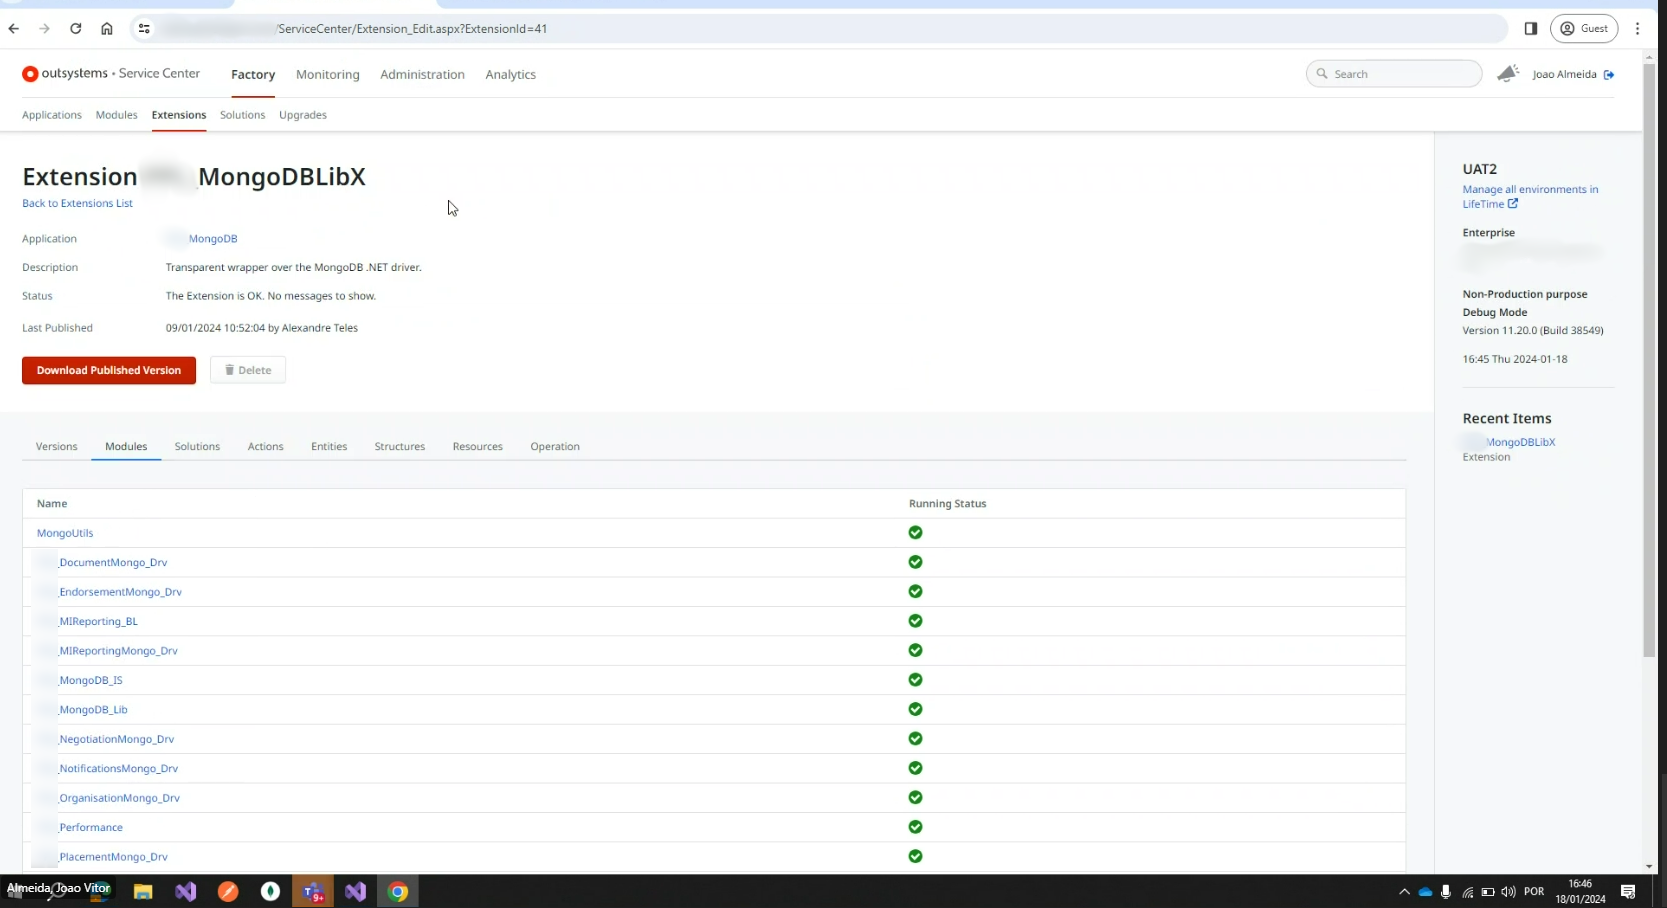
\includegraphics[scale=0.35]{imgs/ExtensionEndpoint-outsystems.png}
                    \caption{Extensão da OutSystems}\label{fig:os-extension}
                    \source{Documentação Interna}
                \end{figure}

            \subsubsection{API Org Config}\label{secsec:api-org-config}
            
                Desenvolvido em .NET fora de OutSystems, o papel do Org Config é ter um método de comunicar com mongoDB, Nuxeo, Azure e OutSystems de forma consistente, garantindo não haver dessincronização entre os dados.

                Por exemplo, o registo dos utilizadores que existem em cada ambiente e as suas permissões devem constar da base de dados MongoDB, o principal sítio que mantém os dados dos utilizadores, no Nuxeo, para que um documento de um cliente possa ser acedido apenas por esse cliente e o URL não seja público. \\
                Estão guardados também no Azure, para efeitos de análise de dados e erros.

                Desta forma o processo é simplificado, exportando a lógica de sincronização entre vários serviços para o API Org Config, que disponibiliza a lógica em mais de uma dúzia de funções visiveis na Figura \ref{fig:api-org-config}.

            \begin{figure}[htbp]
                \centering
                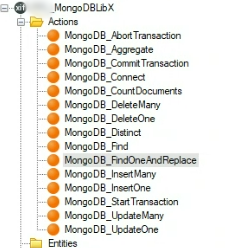
\includegraphics[scale=0.80]{imgs/API-Org-Config.png}
                \caption{Usable actions by the API}\label{fig:api-org-config}
                \source{Documentação Interna}
            \end{figure}
        
        \subsection{Versionamento}\label{secsec:versionamento}

            Como alternativa à utilização de uma ferramenta direta de controlo de versionamento, foi elaborado um sistema de vários ambientes, cada um com uma função específica, por onde o código viaja antes de finalmente se encontrar no ambiente final de produção usado pelos utilizadores.
        
            Os números das versões regem-se por majors, minors e hotfixes.

            \[
                \text{Version: }
                  \underbrace{2\vphantom{(y)}}_\text{major} \text{.}
                  \underbrace{3\vphantom{(y)}}_\text{minor} \text{.}
                  \underbrace{5\vphantom{(y)}}_\text{hotfix} \text{.}
              \]

            \begin{itemize}
                \item \textbf{Major:} A versão principal que indica grandes atualizações ou alterações no software. Aumentar o número da versão principal implica mudanças significativas como, por exemplo, uma reestruturação da plataforma e pode resultar em incompatibilidades com versões anteriores;

                \item \textbf{Minor:} Reflete atualizações menores, melhorias ou adições em partes focadas da aplicação, como, por exemplo, alteração do fluxo para criar um contrato;

                \item \textbf{Hotfix:} Uma correção rápida para resolver problemas críticos, bugs ou \textit{defects}. A diferença entre hotfixes não costuma ser significativa, pelo que não é geralmente referida. Quando se menciona a versão da plataforma, geralmente inclui-se apenas da major e da minor, por exemplo: Versão 2.3.
                
            \end{itemize}
            
            \subsubsection{Ambientes}\label{secsec:ambientes}

                Nesta seção, apresenta-se uma visão abrangente dos ambientes envolvidos no processo de desenvolvimento, teste e implementação.

                É crucial compreender o propósito de cada ambiente para garantir uma implementação eficaz da metodologia AD Factory. A Tabela \ref{table:desc-ambinetes} oferece uma descrição detalhada dos diferentes ambientes, destacando a sua utilização principal e os principais utilizadores envolvidos.

                \textbf{AD Factory}: A AD Factory (Application Development Factory) representa uma abordagem organizada no projeto, focada na estruturação eficiente do ciclo de desenvolvimento. Divide-se em várias linhas de trabalho (PODs) que se refletem em várias equipas, a AD Factory coordena desde a fase de design até aos testes num processo estruturado. Durante a fase de design, as decisões detalhadas são tomadas em cada POD, com histórias de utilizadores aprovadas por um Analista de Dados de Negócios (BDA). A fase de construção e testes seguem-se conforme planos elaborados em sessões de \textit{sprint}, utilizando quadros JIRA específicos para cada POD. Acompanha-se o progresso através do JIRA, com relatórios, fluxos principais e a lista de \textit{defects} bem categorizados.

                \begin{table}[htbp]
                    \centering
                    \caption{ Descrição dos ambientes }\label{table:desc-ambinetes}
                    \source{Documentação Interna}
                    \begin{tblr}{
                    colspec={|X|X[3]|X[1]|}, row{1} = {c}, hlines={lightgray}, vlines={lightgray},
                    }
                    \textbf{Ambiente} & \textbf{Descrição / Uso} & \textbf{Principais Utilizadores} \\
                    %DEV
                    Desenvolvimento (DES) & Ambiente de desenvolvimento para desenvolver as ``User Stories''. & Programadores \\
                    %STG
                    Teste (TES1) & Utilizado para teste de sistema com DES, integração e regressão. & Programadores e Tests na sprint \\
                    %DAD
                    Desenvolvimento para AD Factory (DED) & Ambiente para apoiar o desenvolvimento do ramo de código AD Factory em paralelo com as correções e correções de bugs no ramo DES. & Programadores da AD Factory \\
                    %SAD
                    Teste para AD Factory (TES2) & Ambiente temporário para apoiar os testes do ramo DED. & Programadores da AD Factory e Testes na sprint \\
                    %E2E
                    Ponta a Ponta (P2P) & Utilizado para testes ponta a ponta de temas discutidos nas \textit{sprints}. & Equipa de Testes E2E \\
                    %UAT
                    Aceitação do Utilizador (ADU) & Utilizado para testes de aceitação do utilizador. Teste de upload de configuração da organização e verificação de processos com empresas. & Equipa de Testes da RIL \\
                    %PERF
                    Performance (PCE) & Utilizado para testes de desempenho. & Equipa de Testes de Performance \\
                    %PRE
                    Pré-Produção (PREP) & Ambiente para auxiliar o ambiente PRO, para testes, configuração, testes de mercado e integração de APIs. & Equipa de Testes de Mercado da RIL \\
                    %JIT
                    Teste Integração Conjunta (TIC) & Utilizado para integração do mercado com a API exposta externamente. & Devs e entidades externas \\
                    %DEMO
                    Demonstração (SHOW) & Ambiente com cópia de PRO para efeitos de demonstração. & Gestão de Relações RIL \\
                    %SUP
                    Produção de Suporte (AUX) & Ambiente publicado com uma versão do código de produção quase idêntico, permitindo solucionar problemas sem impactar o ambiente de produção. & Equipa de Execução \\
                    %PRDO
                    Produção (PRO) & Ambiente de produção disponível aos clientes. Testes de Aceitação Operacional. Teste de Penetração da RIL. & Clientes da RIL, administradores da RIL e Equipa de Execução \\
                    \end{tblr}
                \end{table}

            \subsubsection{\textit{Deployment Agreggator}}\label{secsec:deployment-agreggator}

            \begin{figure}[htbp]
                \centering
                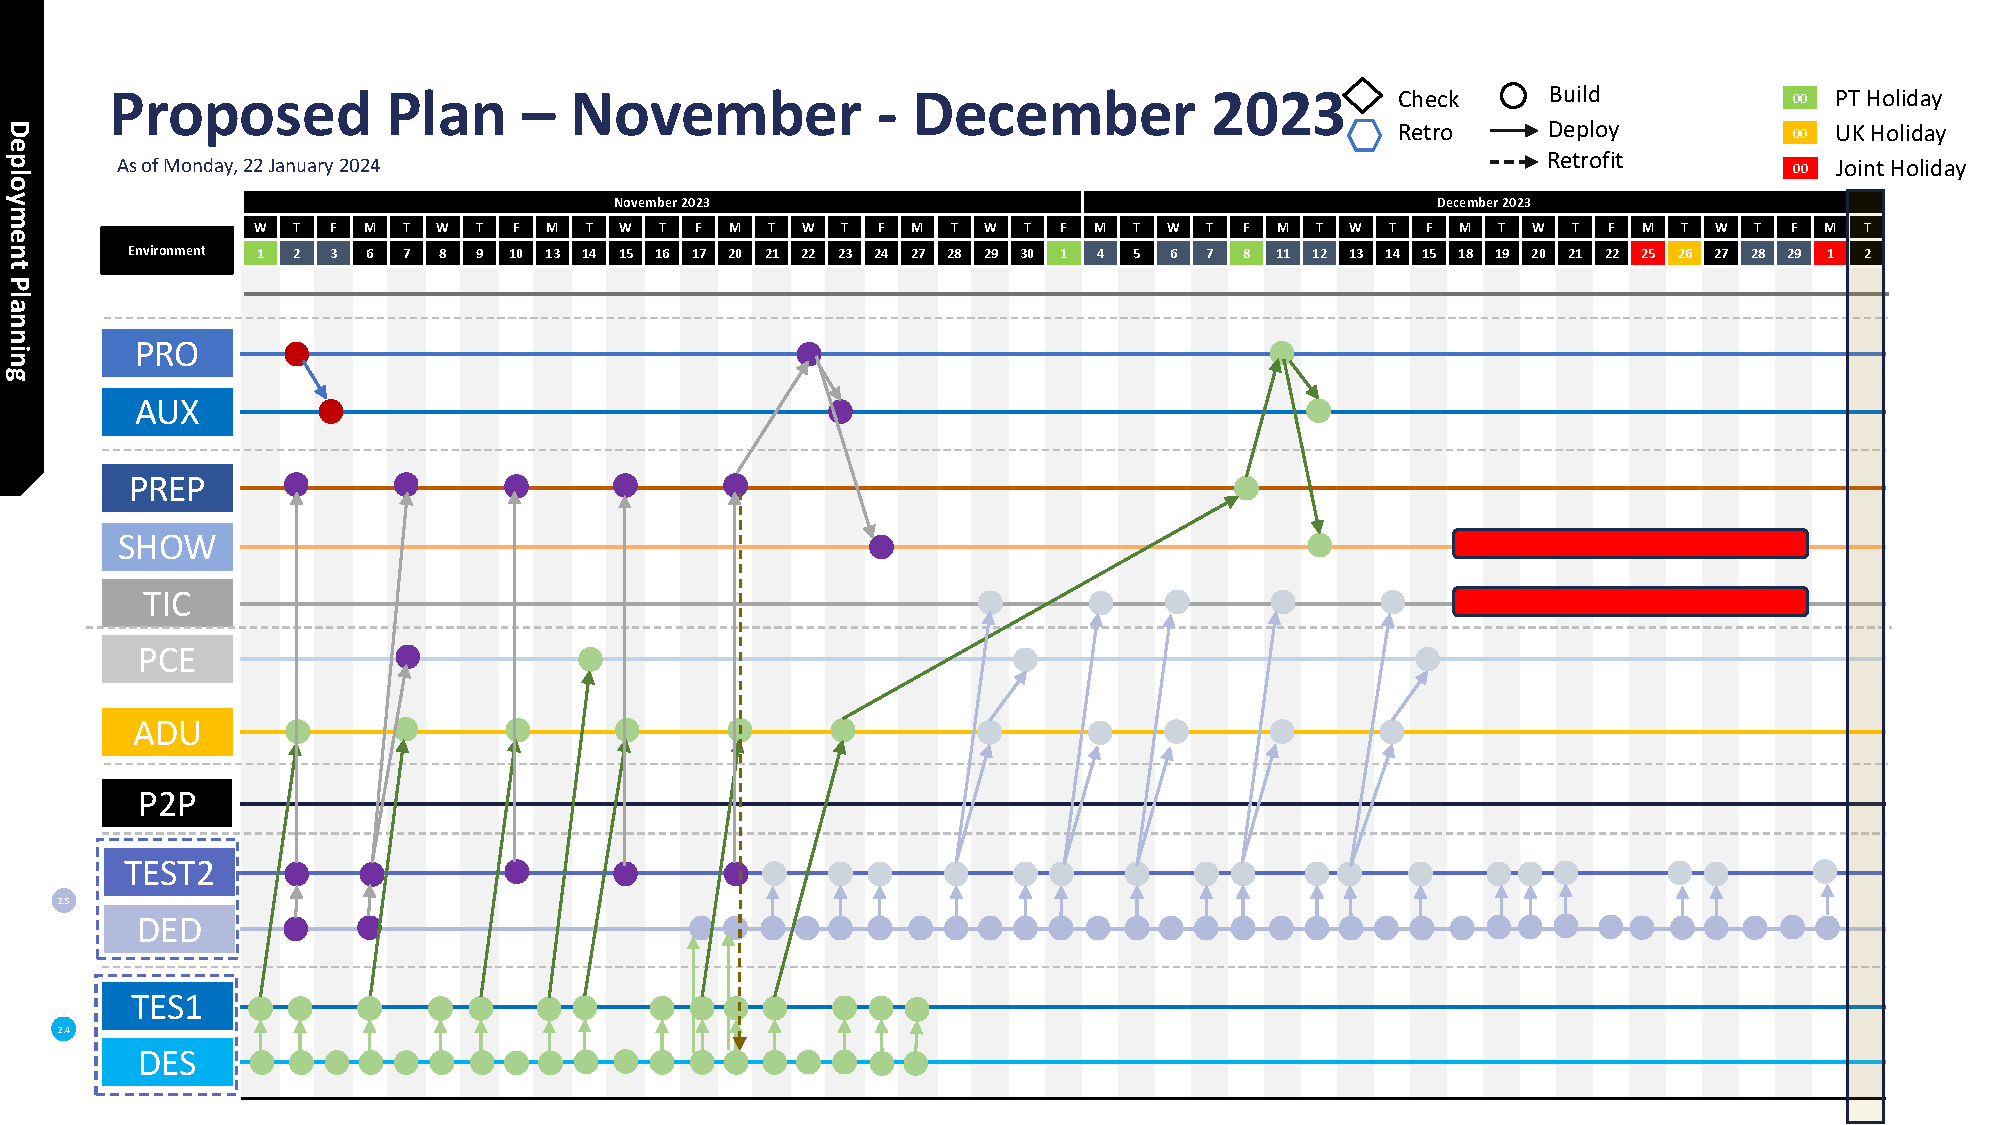
\includegraphics[width=\textwidth]{imgs/DeploymentAggregator-Example.pdf} % You can replace 'example-image-a' with the path to your actual image
                \caption{\textit{Deployment Aggregator}}\label{fig:deployment-aggregator}
                \source{Protótipo de um \textit{Deployment Aggregator} com base na Documentação Interna}
            \end{figure}

            A cada par de meses, é gerado um novo ``Deployment Aggreggator'', um cronodiagrama que detalha o fluxo do código entre ambientes e as datas em que estes \textit{deploys} devem ocorrer.
             
            Pode ter também a representação de férias ou freezes, um paradigma bastante usado em empresas, que se refere a períodos em que não há textit{deploys} e a maior parte dos trabalhadores não estão de serviço, por exemplo, por estarem de férias, podendo, no entanto, haver \textit{deploys} de emergência. Este período é representado por retângulos vermelhos no \textit{deployment} agreggator, Figura \ref{fig:deployment-aggregator}.
            
            Existem dois ambientes de desenvolvimento, neste exemplo, TEST1 e TEST2, ambos com um ambiente de testes, DES e DED, respetivamente. Foram criados os dois para possibilitar o trabalho em duas \textit{sprints} de desenvolvimento, duas minors diferentes, por exemplo, simultaneamente. No protótipo de exemplo dado, está-se a trabalhar na minor 2.4 no ambiente DES e na minor 2.5 no ambiente DED. É possível ver que o código da 2.4 vai chegar a produção no dia 11 de dezembro, e que o código com a 2.5, que irá ser fundido no ambiente ADU, não tem ainda uma data definida para a chegada à produção devido ao freeze.

            % todo: o que é um retrofit tmb

  \section{Ferramentas e Plataformas usadas no desenvolvimento da RIL}

    Nesta secção vão ser analisadas as ferramentas usadas no projeto, e as equipas ou profissionais que normalmente as manuseiam e como.

    \subsection{OutSystems}\label{sec:outsystems}
    
        Estabelecida em 2001, a OutSystems é uma das principais plataformas mencionadas no desenvolvimento \textit{low-code}, foi desenhada com o fluxo empresarial em mente, facilitando a criação e entrega rápida de aplicações. A sua interface de desenvolvimento visual permite a construção de aplicações usando modelos visuais, ações, módulos e blocos reutilizáveis, e diferencia-se oferecendo um conjunto abrangente de ferramentas que cobrem todo o ciclo de vida da aplicação\cite{os-vision}. De seguida são descritos os diferentes ambientes do ecossistema de OutSystems que se usam de forma regular no ambiente de trabalho.
                    
        \subsubsection{Service Studio}

    O Service Studio é o ambiente de desenvolvimento low-code de OutSystems, é onde se criam as aplicações, módulos e a lógica por detrás destas, bem como o desenvolvimento das interfaces de utilizadores para aplicações, quer sejam web tradicionais, web reativas ou móveis. 
    É neste ambiente também que se definem os modelos das bases de dados internas a OS. 
    
    É uma ferramenta muito importante no contexto dário para o desenvolvimento e manutenção cotínua da aplicação.

\subsubsection{Service Center}

    A plataforma oferece uma variedade de configurações que podem ser ajustadas para personalizar o comportamento em diferentes áreas. Estas configurações são ajustáveis a partir do Service Center, permitindo a visualização e gestão de uma panóplia de funcionalidades como módulos e dependências entre eles, gestão das diferentes aplicações do projeto, gestão do versionamento de cada módulo através da publicação da versão desejada. Bem como o ajuste de variáveis globais.
    
    O Service Center é também uma ferramenta essencial para gerir e diagnosticar erros durante o desenvolvimento ou manutenção, permitindo visualizar logs relacionados com timers, processos, módulos, \textit{screen requests}, \textit{service actions}, \textit{traditional web requests}, integrações, extensões ou e-mails.

\subsubsection{Lifetime}

    O Lifetime é uma plataforma do ecossistema de OutSystems que gere o ciclo de vida completo das aplicações. Proporciona visibilidade total sobre os diferentes ambientes, desde o desenvolvimento até à produção, sendo a ferramenta principal na realização de \textit{Deployments}, resolvendo conflitos e efetuando \textit{merges} automaticamente sempre que possível e ajudando o utilizador no processo em caso de conflitos. Oferece, além disso, funcionalidades para versionamento e migração.

        \subsubsection{Um Guia de Boas Práticas de Código para OutSystems}\label{secsec:um-guia-de-estilo-de-codigo}

    Todas as linguagens de programação bem estabelecidas têm diretrizes de programação tão bem enraizadas na cultura da língua que são ensinadas em conjunto com ela, desta forma, com os profissionais a aplicar um método parecido no desenvolvimento do código tem-se um projeto muito mais coerente.

    No entanto, OutSystems carece de um guia de diretrizes estabelecido. Isto deve-se principalmente ao facto de OutSystems ser radicalmente diferente de outras linguagens de programação, sendo um paradigma visual onde até a interface pode ser modificada, não existe um consenso universal para a forma como o código deva ser organizado visualmente.

    Neste capítulo vamos explorar algumas das diretrizes que nos foram introduzidas e aconselhadas a seguir quando alterássemos código na aplicação. Estas indicações começaram a ser introduzidas recentemente, pelo que muito do código existente não cumpre estas normas, mas há um incentivo para uniformizar o código da aplicação.

    \textbf{Diretriz 1 — Sentido descendente é progresso:} Figura \ref{fig:diretriz1}, o sentido descendente deve levar-nos ao objetivo da ação. Este é o sentido de leitura geralmente acordada, até por diferentes culturas;

    \textbf{Diretriz 2 — Ramificações para a direita:} Figura \ref{fig:diretriz2}, o ramo mais importante de um ``if'' deverá seguir da esquerda para a direita. Um nodo ``if'' geralmente tem um ramo que se espera ser executado com mais frequência ou o ramo que é simplesmente mais importante a termos de valor comercial. Este ramo deve mover-se para a direita, e o outro deve continuar reto para baixo;

    \begin{figure}[H]
        \centering
        \begin{minipage}{.5\textwidth}
            \centering
            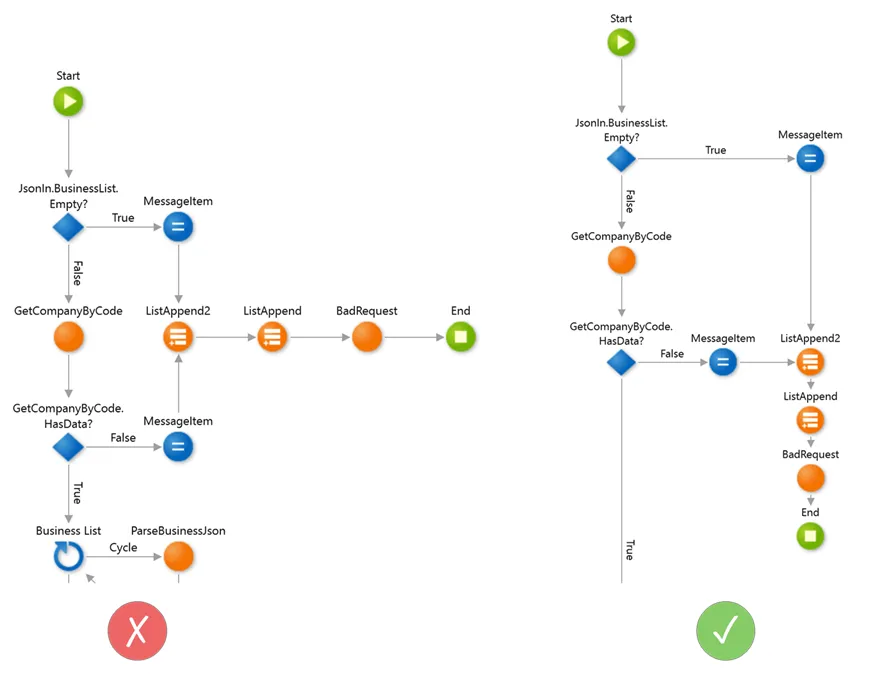
\includegraphics[scale=0.35]{imgs/diretrizes/1.png}
            \caption{Diretriz 1 — Sentido descendente é progresso}\label{fig:diretriz1}
            \source{\cite{outsystems-style-guide}}
        \end{minipage}%
        \begin{minipage}{.5\textwidth}
            \centering
            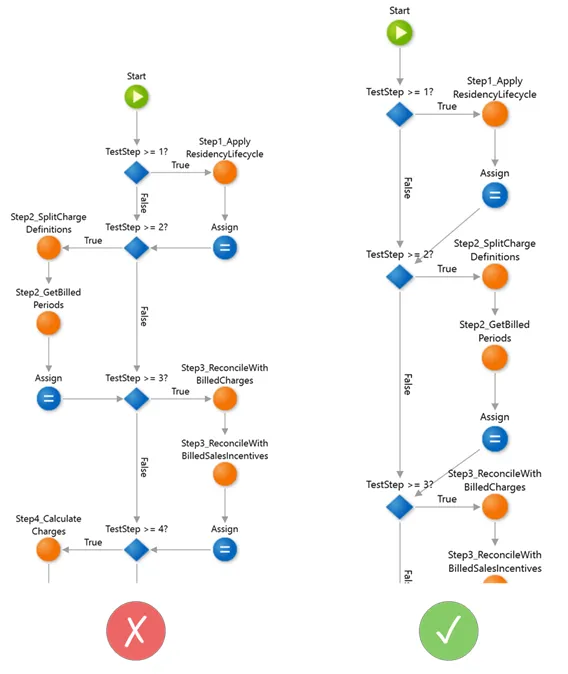
\includegraphics[scale=0.40]{imgs/diretrizes/2.png}
            \caption{Diretriz 2 — Ramificações para a direita}\label{fig:diretriz2}
            \source{\cite{outsystems-style-guide}}
        \end{minipage}
    \end{figure}

    \textbf{Diretriz 3 — Exceções para a direita:} Figura \ref{fig:diretriz3}, exceções para a direita, mesmo que não seja o ramo ``mais importante''. Se se aplicasse a diretriz 2 às exceções, acabava-se com um código maioritariamente horizontal, desta forma impede-se que a exceção se destaque, e mantém-se o foco no código principal;

    \textbf{Diretriz 4 — Ciclos:} Figura \ref{fig:diretriz4}, os ciclos devem iniciar-se numa diagonal para cima e para a direita;

    \begin{figure}[htbp]
        \centering
        \begin{minipage}{.5\textwidth}
            \centering
            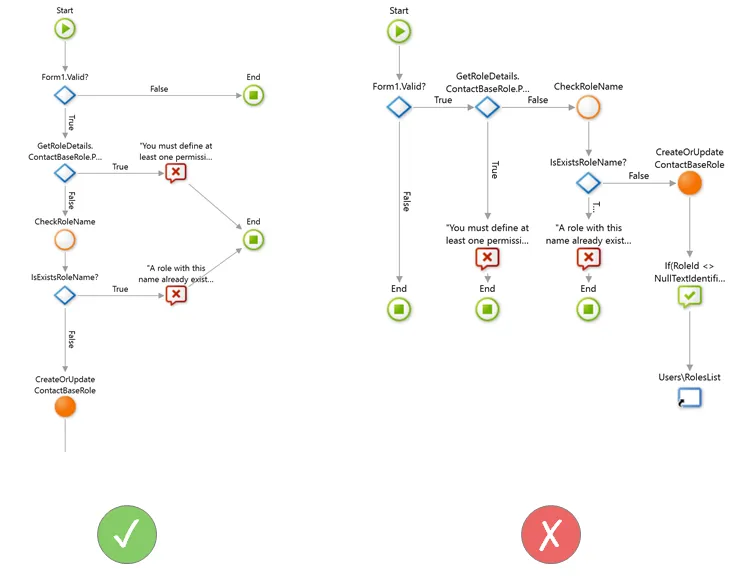
\includegraphics[scale=0.40]{imgs/diretrizes/3.png}
            \caption{Diretriz 3 — Exceções para a direita}\label{fig:diretriz3}
            \source{\cite{outsystems-style-guide}}
        \end{minipage}%
        \begin{minipage}{.5\textwidth}
            \centering
            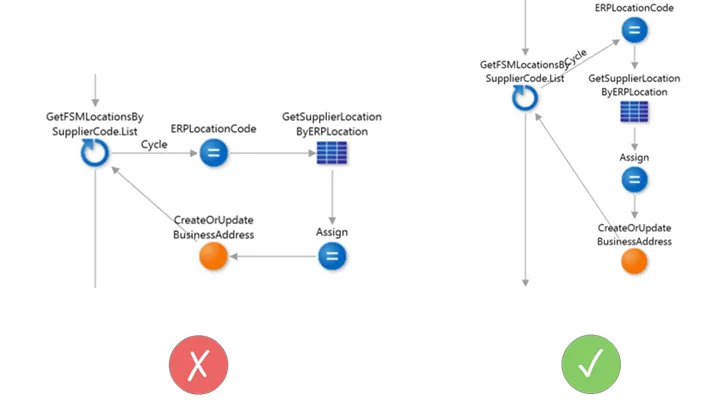
\includegraphics[scale=0.32]{imgs/diretrizes/4.png}
            \caption{Diretriz 4 — Ciclos}\label{fig:diretriz4}
            \source{\cite{outsystems-style-guide}}
        \end{minipage}
    \end{figure}

    \textbf{Diretriz 5 — Evitar setas sobrepostas:} Figura \ref{fig:diretriz5}, as setas sobrepostas devem ser evitadas mesmo que implique ignorar outra diretriz, se for necessário deve-se criar nodos ``dummy'' para direcionar as setas de forma a que não se sobreponham;

    \textbf{Diretriz 6 — Alinhar com intenção:} Figura \ref{fig:diretriz6}, alinhar intencionalmente os nodos relacionados entre si. Por exemplo, se dois ramos têm código similar, os nodos iguais devem estar alinhados horizontalmente para ser ver que será o mesmo código;

    \begin{figure}[htbp]
        \centering
        \begin{minipage}{.5\textwidth}
            \centering
            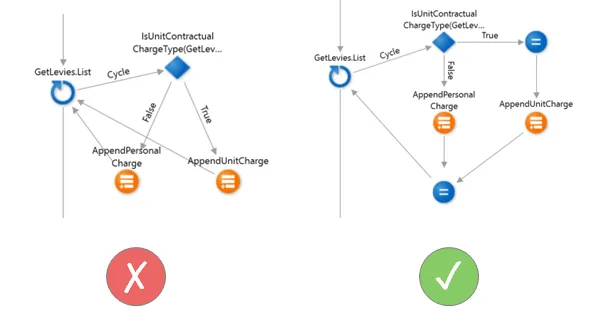
\includegraphics[scale=0.37]{imgs/diretrizes/5.png}
            \caption{Diretriz 5 — Evitar sobreposições}\label{fig:diretriz5}
            \source{\cite{outsystems-style-guide}}
        \end{minipage}%
        \begin{minipage}{.5\textwidth}
            \centering
            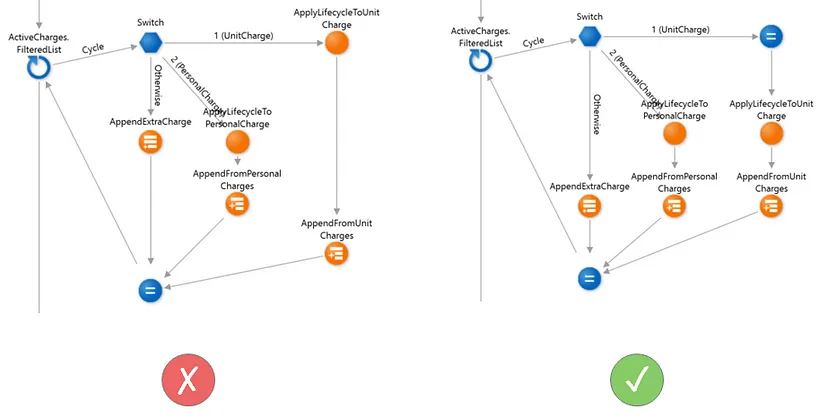
\includegraphics[scale=0.30]{imgs/diretrizes/6.png}
            \caption{Diretriz 6 — Alinhar com intenção}\label{fig:diretriz6}
            \source{\cite{outsystems-style-guide}}
        \end{minipage}
    \end{figure}

    Com estas 6 diretrizes é mais fácil organizar e ler o código da plataforma, e permitirá ter um projeto mais homogéneo e previsível\cite{outsystems-style-guide}.

    % Outlook e ferramentas de desenvolvimento


    % todo, in the Infrestrutura tecnologica na secção que fala de Atlas, referencia também esta secção

        \subsubsection{Competidores}\label{secsec:competidores}

    No ecossistema de desenvolvimento \textit{low-code}, existem várias plataformas que competem com OutSystems. A escolha entre estas dependerá das necessidades específicas de cada projeto, das preferências da equipa e das metas da empresa. 

    Apesar de OutSystems ser uma das plataformas mais maduras e bem desenvolvidas para este fim no mercado, podemos fazer uma análise dos seus pontos fortes e fracos:

    \textbf{Pontos Fortes:}
    \begin{itemize}
        \item O Controlo de versionamento pode ser integrado com Git e plataformas como GitHub ou GitLab;
        \item Várias opções para integração com outras plataformas com ferramentas como o \href{https://integrationbuilder.outsystems.com/}{Integration Builder}, desde servidores SQL ao MS SharePoint Online;
        \item Vastas livrarias, pré-definições, e templates disponíveis;
        \item Ênfase também no desenvolvimento de aplicações móveis.
    \end{itemize}

    \textbf{Pontos Fracos:}
    \begin{itemize}
        \item Uma personalização de UI menos flexível em comparação com algumas alternativas;
        \item Flexibilidade para correr os próprios servidores está apenas disponível em alguns planos;
        \item Colaboração não é um dos aspetos mais fortes da plataforma;
        \item Custo comparativamente elevados em relação a outras alternativas\cite{outsystems-vs-mendix}.
    \end{itemize}

    Na Figura \ref{fig:googletrendslowcodeplatforms-ui} pode-se ver algumas das plataformas \textit{low-code} mais usadas nos últimos cinco anos de acordo com o Google Trends e na Figura \ref{tab:lowcode-comparison} como se comparam com as demais.

    \begin{figure}[p] % htbp
        \centering
        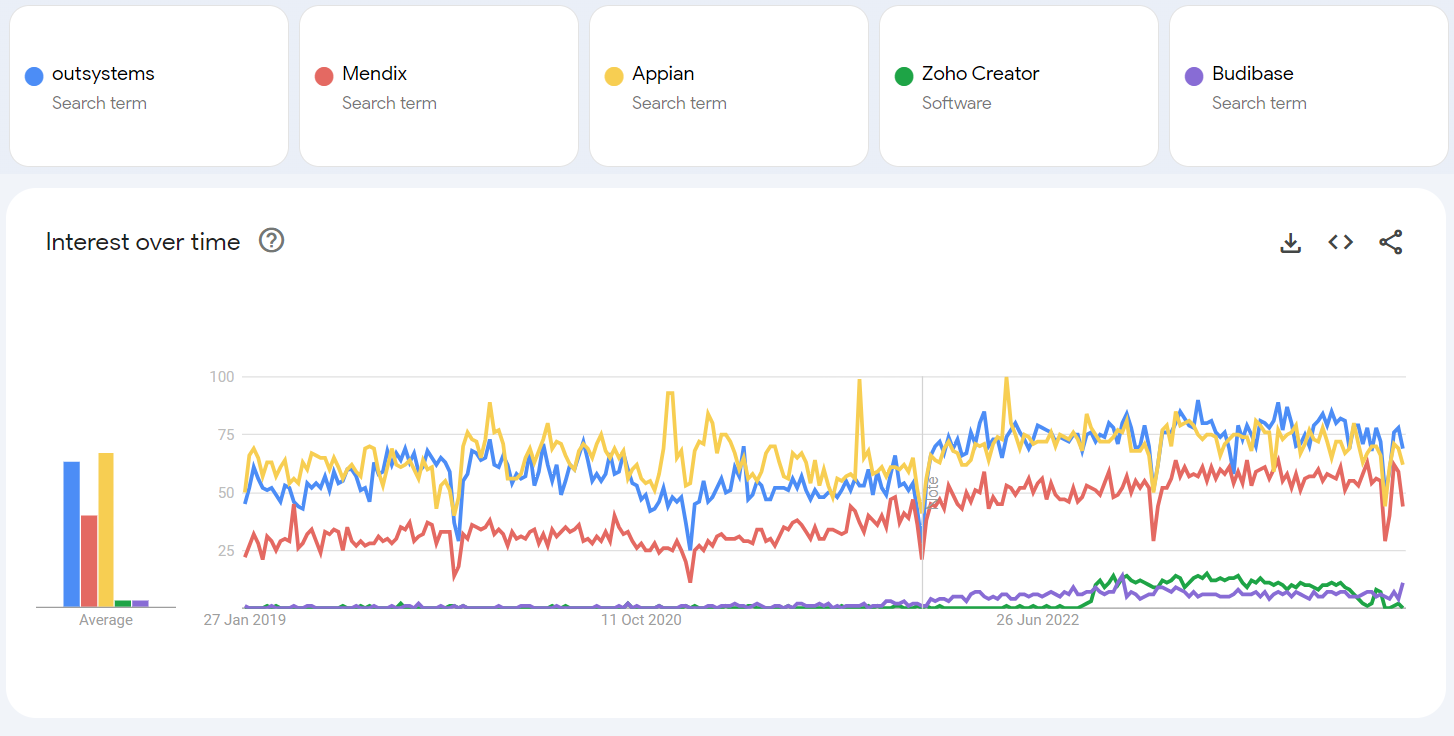
\includegraphics[width=\textwidth]{imgs/GoogleTrendsLowCodePlatforms.png}
        \caption{Google Trends for Low Code Platforms Worldwide}\label{fig:googletrendslowcodeplatforms-ui}
        \source{\cite{g-trends-low-code-platforms}}
    \end{figure}

    % Use this to finish the table: https://impalaintech.com/blog/mendix-vs-outsystems-vs-appian/

    \begin{table}[p] % htbp
        \centering
        \begin{tblr}{
            % example for tblr: https://tex.stackexchange.com/questions/603349/tabularray-and-new-command-for-multicolumn-cells
            % another example: https://tex.stackexchange.com/questions/605676/tabularray-how-to-control-the-vertical-alignment-of-the-cells-contents
            hlines={lightgray}, vlines={lightgray},
            width = \linewidth,% total width set to width available
            %rows = {c,m}, % c aligns horizontally, m aligns vertically, aligns all rows
            colspec={Q[l,m,3cm] X[c,m] X[c,m] X[c,m] X[c,m]},
            cell{1}{1} = {r=2}{c}, % Merge cells in the first row and second row
        }
            \textbf{Campo} & \SetCell[c=4]{c} \textbf{Plataformas} \\
                        & \textbf{OutSystems} & \textbf{Mendix} & \textbf{Appian} & \textbf{Pega} \\ 
            Facilidade de Utilização               & Médio       & Alto        & Alto        & Baixo        \\ 
            Integração                             & Muito Alto  & Alto        & Alto        & Alto        \\ 
            Escalabilidade                         & Muito Alto  & Muito Alto  & Muito Alto  & Muito Alto  \\ 
            % Flexibilidade no Desenvolvimento da UI & Alto        & Muito Alto  & Alto        & Alto        \\  % Para Pega e Appian são as unicas duas que não estão bem fundamentadas
            Foco em Desenvolvimento Móvel          & Alto        & Alto        & Alto        & Alto        \\ 
            Colaboração                            & Alto        & Muito Alto  & Alto        & Alto       \\
            Custo                                  & Alto        & Disponível após Pedido & Alto & Disponível após Pedido  \\
        \end{tblr}
        \caption{Comparação de Plataformas Low-Code}
        \label{tab:lowcode-comparison}
        \source{\cite{mendix-vs-outsystems-vs-appian,outsystems-vs-mendix}} % 1- https://impalaintech.com/blog/mendix-vs-outsystems-vs-appian/
    \end{table}

    O ambiente de desenvolvimento \textit{low-code} é muito competitivo, pelo que existe uma panóplia de ferramentas com objetivos similares, como por exemplo: Bonitasoft, Appsheet, Bubble, Zoho Create, Budibase, Backendless, Eclipse/SAP, Salesforce Lightning, etc. Pode ser que nenhuma das ferramentas aqui analisadas sejam a mais indicada para qualquer projeto. Algumas equipas também adotam abordagens com uma pilha de infraestrutura constituída por vários programas de ecossistemas diferentes, utilizando diferentes ferramentas para aspetos específicos, como Webflow para o front-end e Zappier ou N8n para o lado do servidor. No fundo, esta área é muito flexível e está sempre em constante evolução, e pode ser que a infraestrutura mais indicada para um projeto seja uma que tenha que ser feita à medida.
        
    % Reddit opinion: https://www.reddit.com/r/lowcode/comments/lp9f4p/recommendations_please/
    % Outras: Bonitasoft, Appsheet, bubble, Zoho Create, Budibase, Backendless and Eclipse/SAP, Salesforce Lightning
    % ou uso de várias: Webflow is relatively powerful for a front-end, Zappier or N8n (free) - for the server side, and some database (tool) - Airtable/Firebase/Backendless - for the data.
    % outra dessas arranjei aqui: https://www.outsystems.com/forums/discussion/86088/outsystems-vs-other-low-code-platforms/

    % Another reddit opinion: https://www.reddit.com/r/lowcode/comments/lp9f4p/recommendations_please/


    \subsubsubsection{Mendix}\label{secsecsec:mendix}
        
        Fundada em 2005, a Mendix é uma plataforma de desenvolvimento \textit{low-code} projetada para fornecer às empresas ferramentas para rapidamente construir e distribuir aplicações personalizadas. Os fundadores acreditavam que o desenvolvimento e a distribuição de software iria beneficiar bastante com uma mudança de paradigma, e daí nasceu a empresa. Mendix foca-se na colaboração permitindo às equipas trabalhar efetivamente em conjunto e simplificando o desenvolvimento através de modelagem visual com uma interface intuitiva, como visivel na Figura \ref{fig:mendixui-ui}, e componentes reutilizáveis\cite{why-was-mendix-founded}.

        O Mendix destaca-se pela sua flexibilidade enquanto mantém um bom nível de intuição. Oferece também um mercado privado de aplicações que permite a sua partilha mesmo internamente. Proporciona uma variedade de opções de implementação, incluindo diferentes serviços cloud, soluções locais e híbridas, adaptando-se sempre às diversas necessidades da organização\cite{outsystems-vs-mendix}.

        \begin{figure}[htbp] % htbp
            \centering
            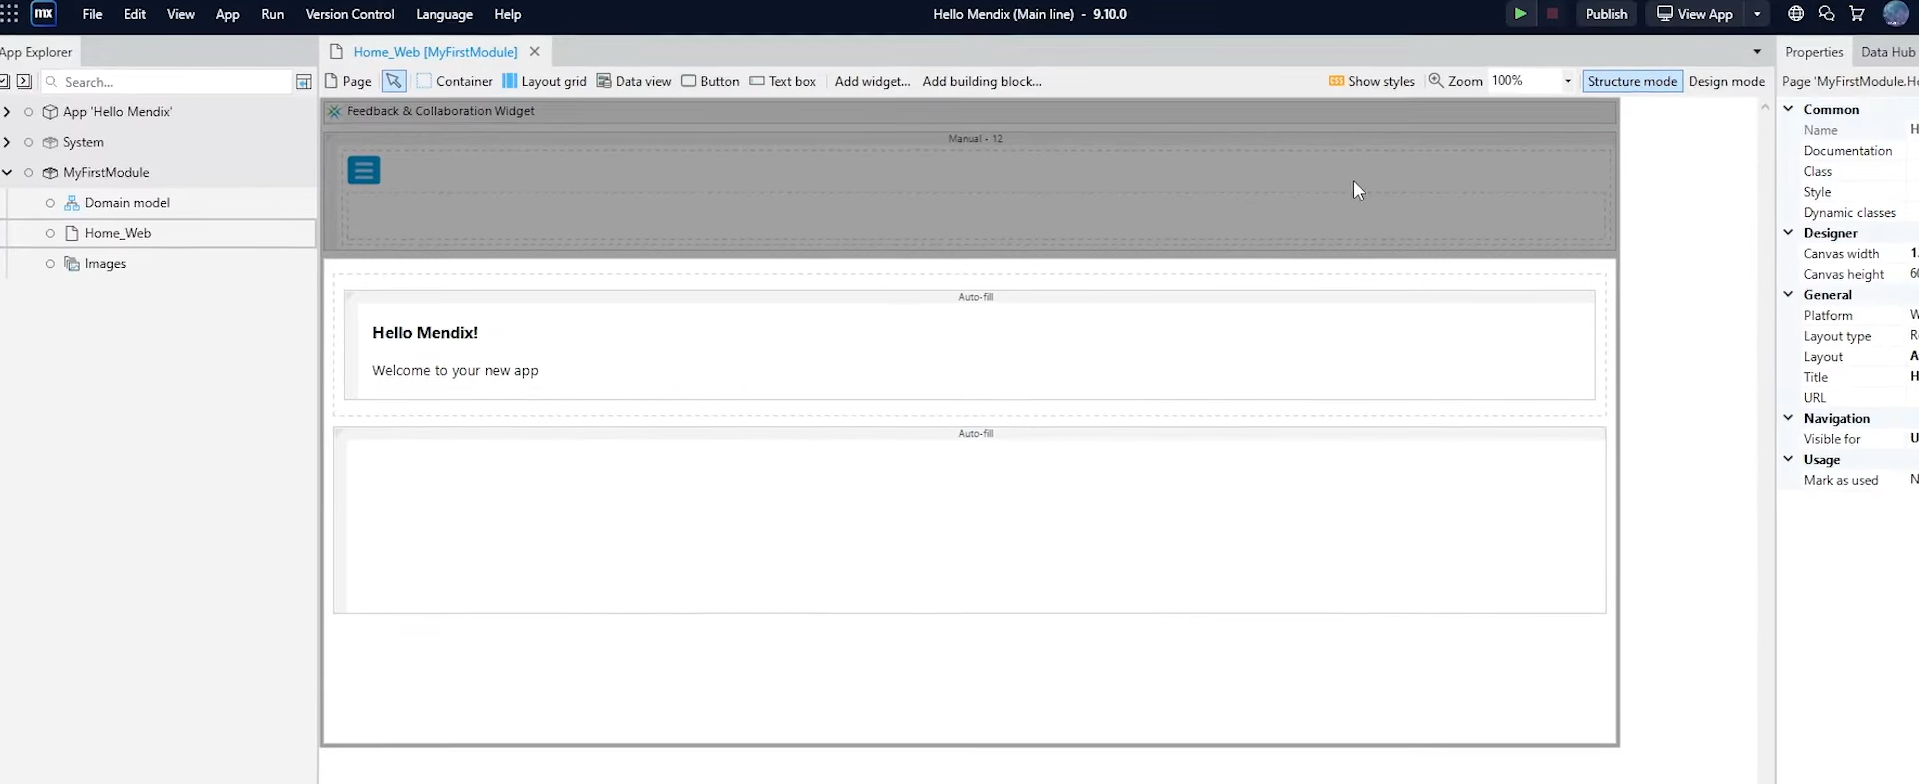
\includegraphics[width=\textwidth]{imgs/MendixUI.png}
            \caption{Mendix UI}\label{fig:mendixui-ui}
            \source{\cite{mendix-ui}}
        \end{figure}

        % https://www.appsmith.com/blog/mendix-vs-outsystems

    \subsubsubsection{Appian}\label{secsec:appian}

        Fundada em 1999 por Michael Beckley, Robert Kramer, Marc Wilson e Matthew Calkins e com uma interface como observável na Figura \ref{fig:appian-ui}, a Appian é uma plataforma de desenvolvimento \textit{low-code} criada com o objetivo de simplificar e acelerar o processo de desenvolvimento de software e com a visão de que pessoas talentosas e com paixão, quando proporcionadas com as ferramentas certas irão dar resultados incríeis\cite{appian-company-history,appian-company-overview}. 
    
        \begin{figure}[htbp] % htbp
            \centering
            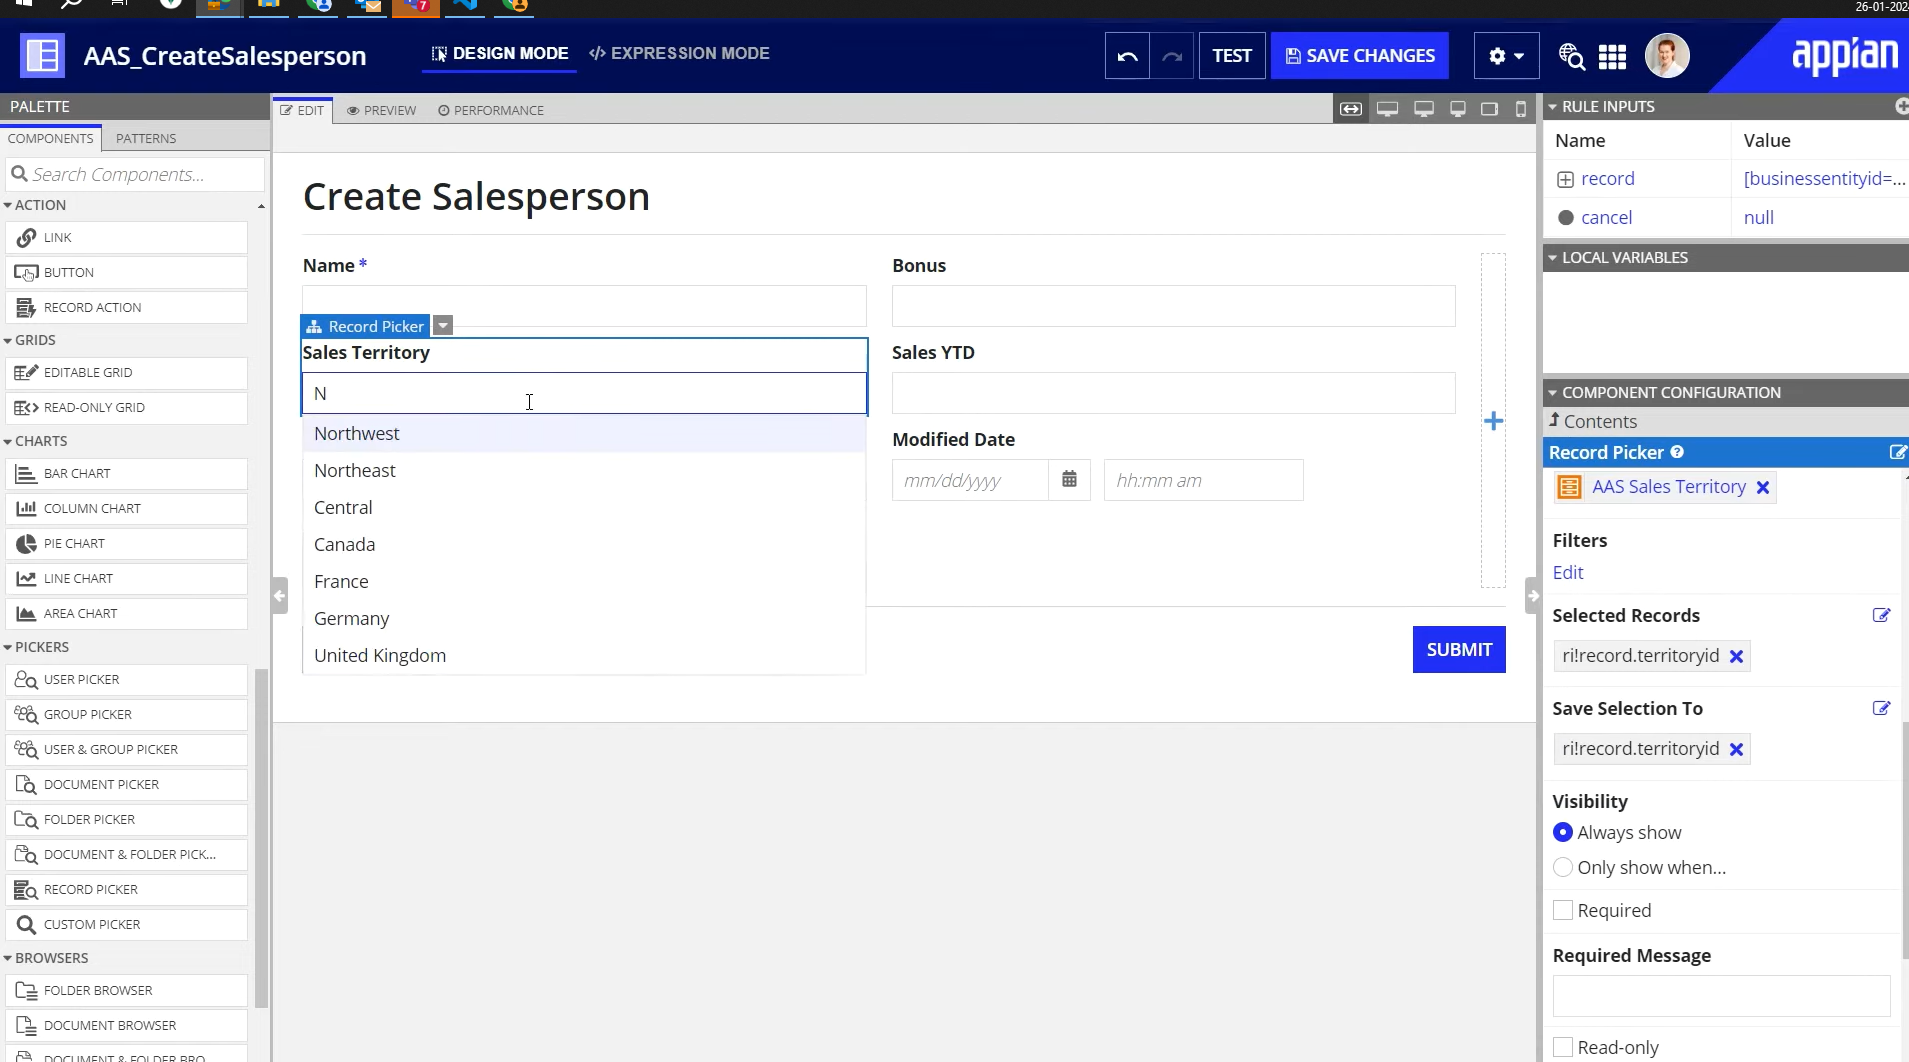
\includegraphics[width=\textwidth]{imgs/AppianUI.png}
            \caption{Appian UI}\label{fig:appian-ui}
            \source{\cite{mendix-ui}}
        \end{figure}

        Appian destaca-se no mercado de desenvolvimento de software devido a várias funcionalidades distintas. Algumas delas incluem:
        
        \begin{enumerate}
            \item \textbf{Deployment Eficiente:}
                \begin{itemize}
                    \item Permite a implantação rápida de aplicações com variadas ferramentas de implantação;
                    \item Oferece a sua própria solução para controlo de versionamento.
                \end{itemize}
            
            \item \textbf{Vários Formatos para Apresentação de Dados:}
                \begin{itemize}
                    \item Possibilita apresentar dados em vários formatos, como tabelas, gráficos em formato grade e PDF.
                \end{itemize}
            
            \item \textbf{Desenvolvimento Visual:}
                \begin{itemize}
                    \item Programadores podem moldar fluxogramas para criar diagramas de processos de forma visual, eliminando a necessidade de codificar manualmente.
                \end{itemize}
            
            \item \textbf{Pontos a Considerar (Desvantagens):}
                \begin{itemize}
                    \item Processo de documentação precisa de ser aprimorado;
                    \item Limitações na integração com outros produtos;
                    \item A ferramenta de gestão de permissões pode ser um pouco lenta;
                    \item Desenvolvimento geral de aplicações pode ser mais lento em comparação com as alternativas analisadas.
                \end{itemize}
        \end{enumerate}
        
        Appian destaca-se na eficiência da implantação de aplicações e na criação de processos através de fluxogramas visuais. A sua flexibilidade na apresentação de dados, em junção com a capacidade de desenvolver aplicações para diversos setores, fazem dela uma opção bastante versátil\cite{mendix-vs-outsystems-vs-appian}.

    \subsubsubsection{Pega Platform}\label{secsecsec:pega}
    
        % fundada https://www.pega.com/about/leadership/alan-trefler#:~:text=Inspired%2C%20he%20founded%20Pega%20in,today%20known%20as%20low%2Dcode.

        A Pega Platform, a plataforma mais antiga das analisadas, fundada em 1983, foi criada por Alan Trefler, um programador na área financeira e dos seguros, fundou Pega devido à desconexão que existia entre os métodos tecnológicos usados e os processos e objetivos empresariais. Desde então, a plataforma tem desempenhado um papel crucial no cenário de desenvolvimento de software, fornecendo soluções robustas para diversas necessidades empresariais, a sua interface está representada na Figura \ref{fig:pega-ui}.

        \begin{figure}[htbp] % htbp
            \centering
            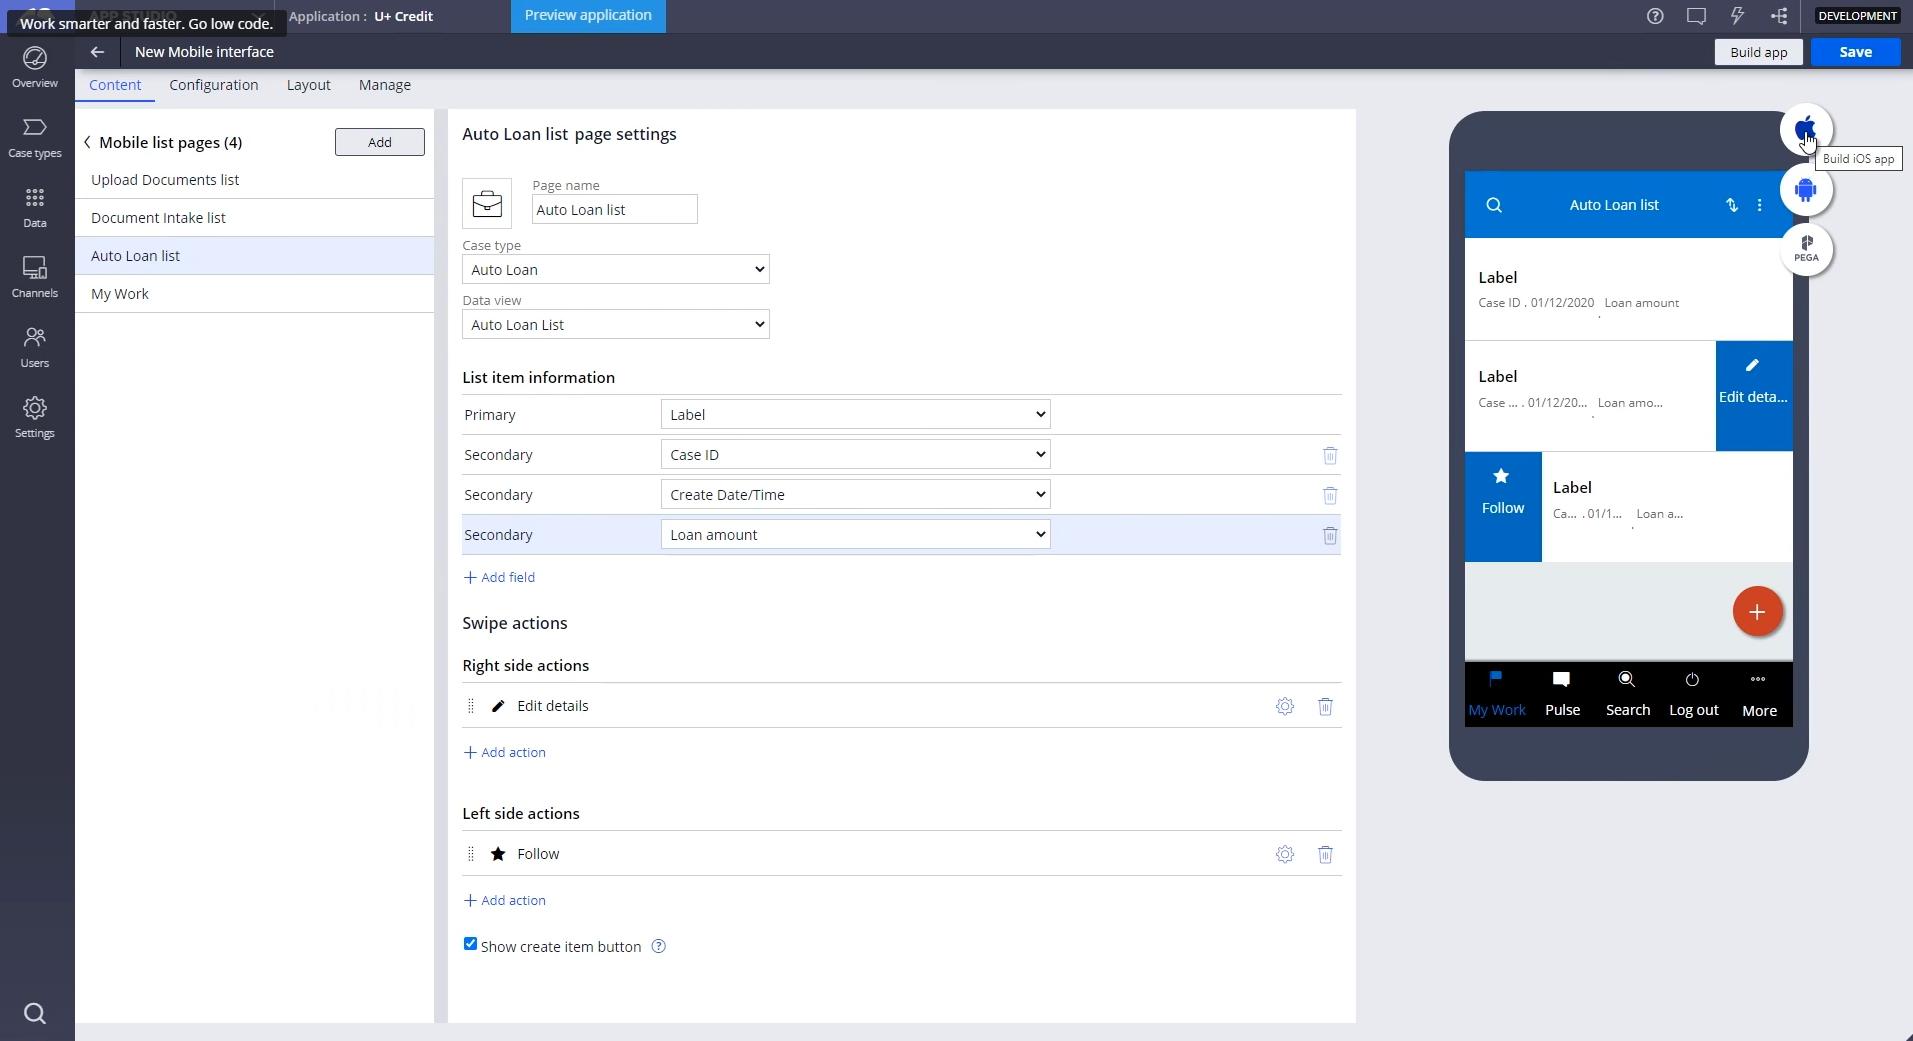
\includegraphics[width=\textwidth]{imgs/PegaUI.png} % You can replace 'example-image-a' with the path to your actual image
            \caption{Pega UI}\label{fig:pega-ui}
            \source{\cite{pega-ui}}
        \end{figure}

        Algumas vantagens e desvantagens da plataforma incluem:
    
        \begin{itemize}
        \item \textbf{Vantagens:}
            \begin{itemize}
            \item Oferece uma abordagem eficiente na gestão de casos, utilizando um modelo central que permite controlar tarefas, contribuindo para uma integração forte com os paradigmas das empresas\cite{o-que-e-gestao-de-casos-pega};
            \item Forte capacidade de incorporar e utilizar inteligência artificial nas aplicações.
            \end{itemize}
        
        \item \textbf{Desvantagens:}
            \begin{itemize}
            \item Tem uma curva de aprendizagem mais acentuada.
            \end{itemize}
        \end{itemize}    

    \subsection{ServiceNow}\label{sec:service-now}

        \begin{figure}[htbp]
            \centering
            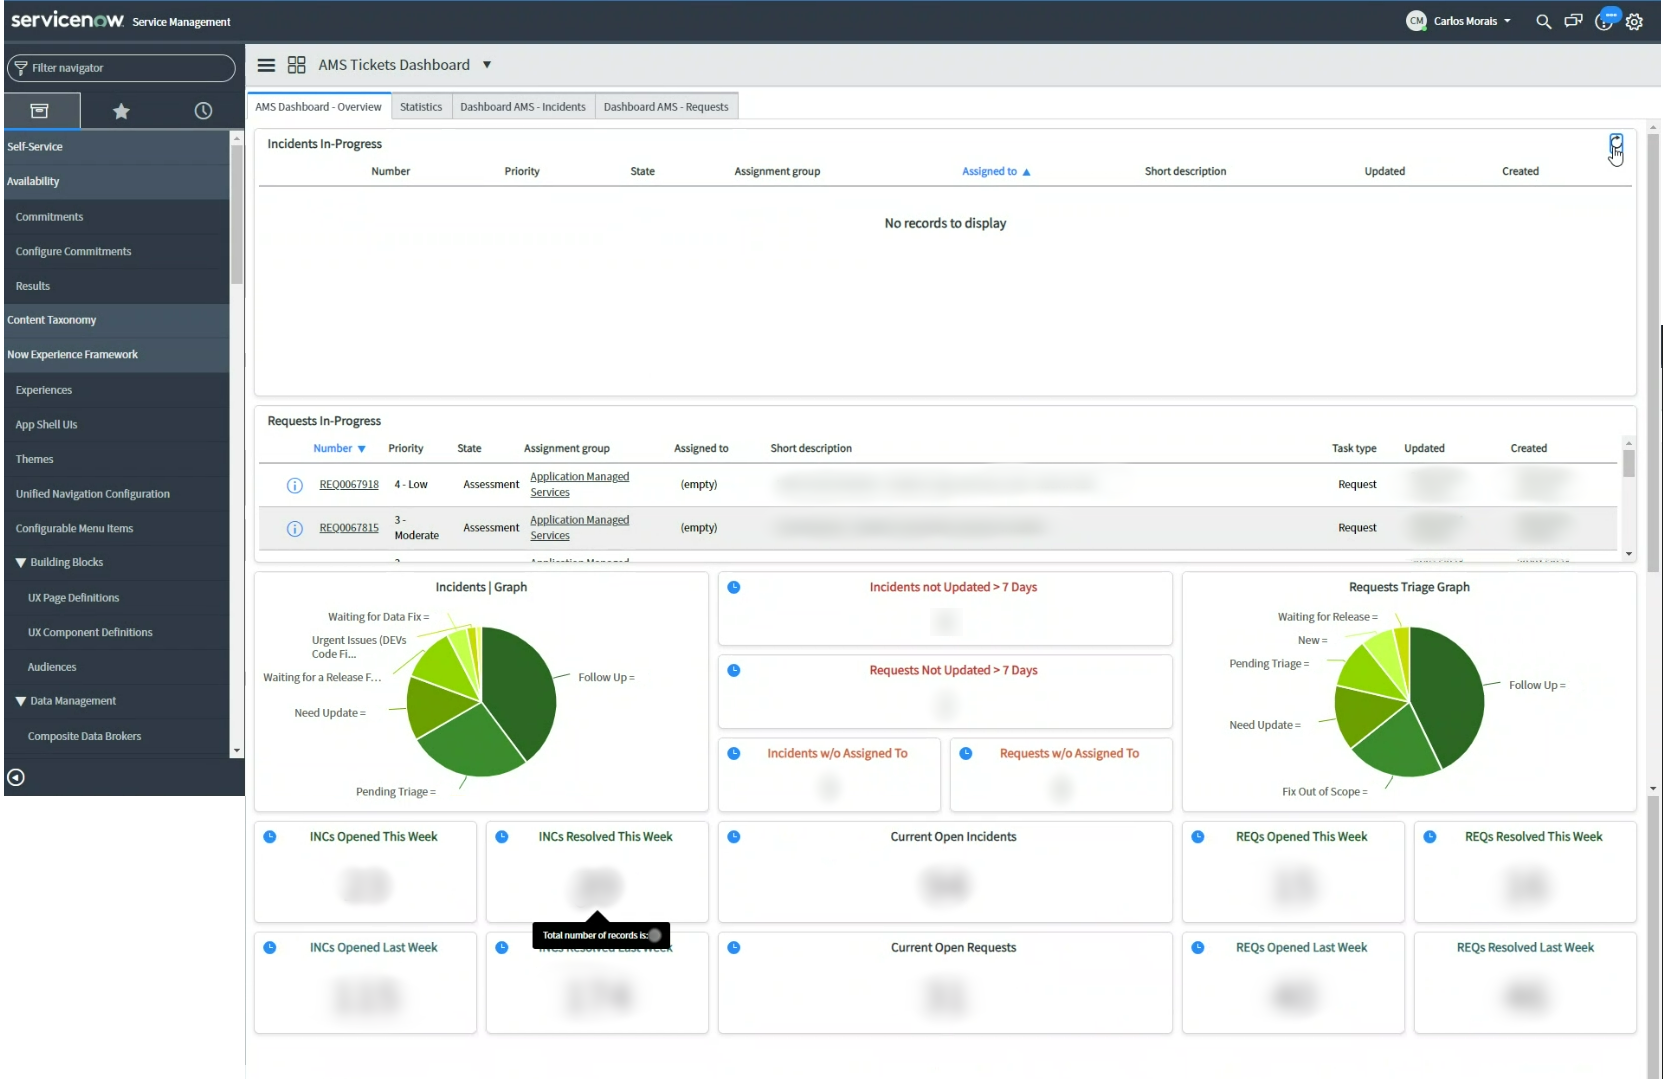
\includegraphics[width=\textwidth]{imgs/ServiceNow.png} % You can replace 'example-image-a' with the path to your actual image
            %\caption{Plataforma ServiceNow - Pagina Principal}
            \caption[Plataforma ServiceNow - Pagina Principal]{Plataforma ServiceNow - Pagina Principal\protect\footnotemark}\label{fig:service-ui}
            \source{Plataforma Interna da ServiceNow}
        \end{figure}
        \footnotetext{Alguma da informação nesta e em próximas imagens será censurada devido a questões de confidencialidade.}

        A ServiceNow é uma das plataformas de referência na gestão de serviços empresariais, oferecendo uma ampla gama de funcionalidades para otimizar e automatizar processos internos. Destaca-se pela sua capacidade de integrar e gerir eficientemente serviços de TI, recursos humanos, gestão de projetos e muito mais, a página principal da aplicação está demonstrada na Figura \ref{fig:service-ui}. Fundada em 2004 pelo antigo CTO da Peregrine Systems, Fred Luddy, ServiceNow iniciou a sua existência num único computador portátil, numa pequena sala de escritório, apoiada por um único colaborador e um punhado de voluntários dedicados.

        No seguimento deste começo, Luddy propôs-se a criar uma plataforma baseada na nuvem para encaminhar o trabalho de forma eficaz, sendo suficientemente poderosa para impulsionar o sucesso empresarial, mas, simultaneamente, simples o suficiente para não afastar potenciais utilizadores. Não é surpreendente que este objetivo tenha chamado a atenção dos clientes. A empresa cresceu rapidamente e, em 2012, tornou-se pública.
        
        Desde então, ServiceNow expandiu significativamente as suas ofertas, e as mesmas prioridades que definiram a sua fundação há vinte anos continuam a defini-lo hoje: uma paixão por fazer as pessoas tirarem mais proveito da tecnologia. 
        
        Atualmente, as ofertas da ServiceNow incluem gestão de serviços de IT, gestão de operações de IT, gestão de serviços ao cliente, gestão de recursos humanos, operações de segurança, risco e conformidade, entrega de serviços no local de trabalho e gestão de serviços de campo - tudo numa só plataforma.

        É através da ServiceNow que os utilizadores reportam os dois tipos de incidentes, request ou incidente, como explicado na secção \ref{sec:terminologia_do_projeto}. De seguida estes passam por uma equipa de suporte que tenta filtrar e resolver os incidentes mais simples, como utilizadores a utilizar mal a plataforma, ou por vezes incidentes que a equipa de desenvolvimento os instruiu a resolver, por exemplo, se um certo problema aparecer, instruam os utilizadores a apagar a cache do browser. Após esta fase, se não foi possível resolver, são enviados para a ServiceNow onde são analisados pelo team leader da equipa em triagem, que manda uma mensagem padrão para o utilizador a pedir desculpas pela inconveniência e a informar que se está investigar o problema, e prioriza os incidentes da seguinte forma:
        \begin{itemize}
            \item \textbf{Low} - Um erro de baixa importância que não bloqueia o utilizador, como uma desformatação do site;
            \item \textbf{Medium} - Quando é mais urgente no sentido de poder afetar a funcionalidade da plataforma, mas haver como contornar o problema, como recarregar a página ou refazer o contrato;
            \item \textbf{High} - Quando o utilizador está bloqueado e não consegue aceder à funcionalidade que necessita. Esta prioridade também pode ser dada a utilizadores de certas organizações maiores, no sentido de serem clientes mais importantes que a empresa quer garantir que mantém;
            \item \textbf{Critical} - Prioridade atribuída a erros urgentes, como erros 502, quando o site está em baixo e ninguém conseguir aceder.
        \end{itemize}
        Seguidamente, ao longo da vida de um incidente este será movido entre um dos seguintes estados, como se pode ver na Figura \ref{fig:servicenow-ui2}:
        \begin{itemize}
            \item \textbf{New:} Novo — O estado inicial de um incidente que acabou de ser recebido;
            \item \textbf{Pending Triage:} Pendente de Triagem — Aguarda avaliação;
            \item \textbf{Waiting for Data Fix:} Aguardando Correção de Dados — À espera que o \textit{datafix}, pedido à equipa da base de dados, seja efetuado;
            \item \textbf{Urgent Issues (DEVs):} Problemas Urgentes (DEVs) — Incidentes críticos que requerem atenção imediata dos programadores;
            \item \textbf{Need update:} Necessita de Atualização — Requer atualização ou informação adicional como por exemplo o UMR (Unique market reference) para identificar o contrato problemático do utilizador;
            \item \textbf{Follow up:} Acompanhamento — À espera de feedback do utilizador para saber se o problema foi resolvido;
            \item \textbf{Follow up second strike:} Acompanhamento segundo golpe — Segundo a política da empresa, após vinte e quatro horas volta-se a mandar mensagem ao utilizador e se nas vinte e quatro seguintes ainda não houver resposta, fecha-se o incidente;
            \item \textbf{Waiting for release:} Aguardando Lançamento — Foi criado \textit{defect} a partir do incidente e espera-se que seja lançada a versão com a correção para produção.
        \end{itemize}
        
        \begin{figure}[htbp]
            \centering
            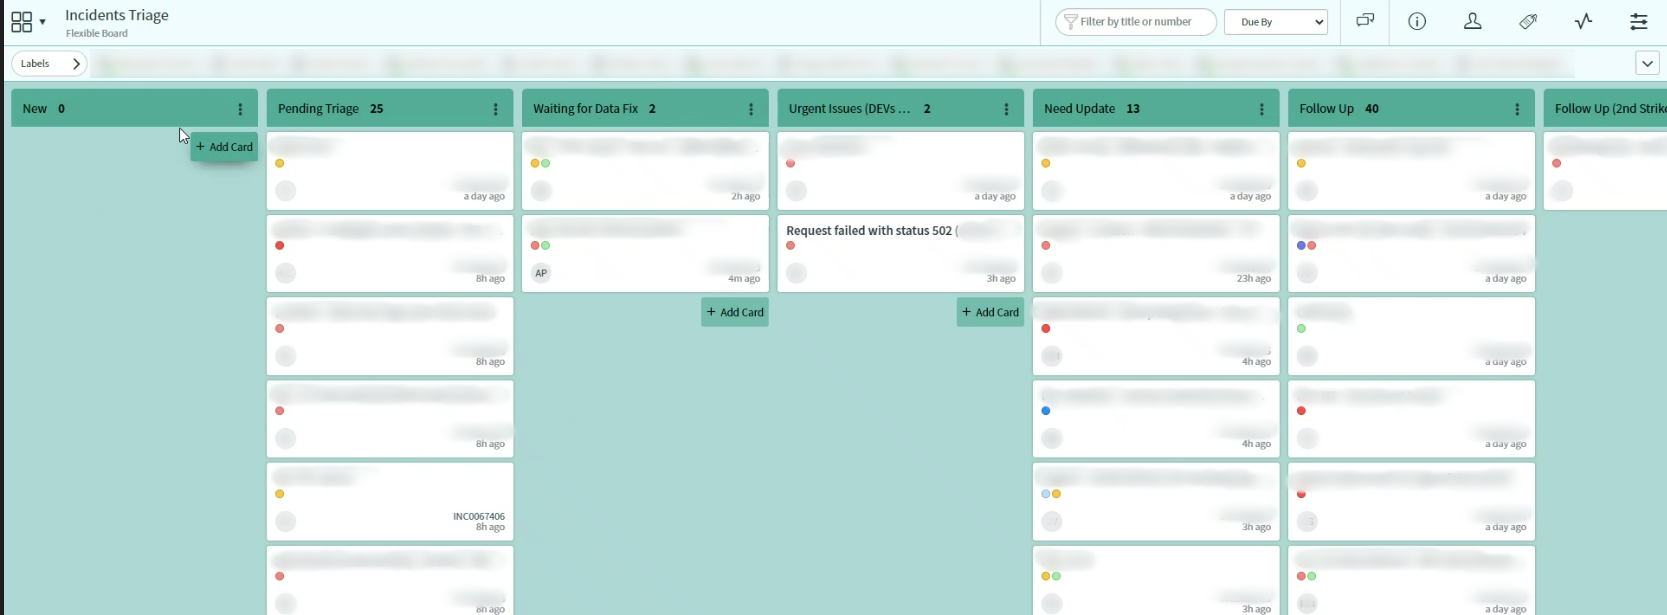
\includegraphics[width=\textwidth]{imgs/ServiceNow2.png}
            \caption{Plataforma ServiceNow - Incidentes}\label{fig:servicenow-ui2}
            \source{Plataforma Interna da ServiceNow}
        \end{figure}

        \subsubsection{Competidores}\label{competidores-service-now} % devo manter, devo arranjar alternativas mesmo? todo
    
            Neste ambiente altamente volátil e de alta competição no desenvolvimento de software empresarial existirão sempre ferramentas que podem substituir funcionalidades de outras, no entanto, no caso da ServiceNow é difícil encontrar uma que faça exatamente o que esta plataforma faz. 
            
            Na realidade o que se alcança com a plataforma ServiceNow pode ser já alcançado pelas ferramentas usadas como o Jira ou Confluence ou por outras como ClickUp[\ref{clickup}], mas a verdadeira vantagem da ServiceNow é a habilidade de ter tudo no mesmo sítio, sendo por isso uma ferramenta única na gestão empresarial.

    \subsection{Plataforma Atlas}\label{sec:ferramentas-atlas}

        \begin{figure}[htbp]
            \centering
            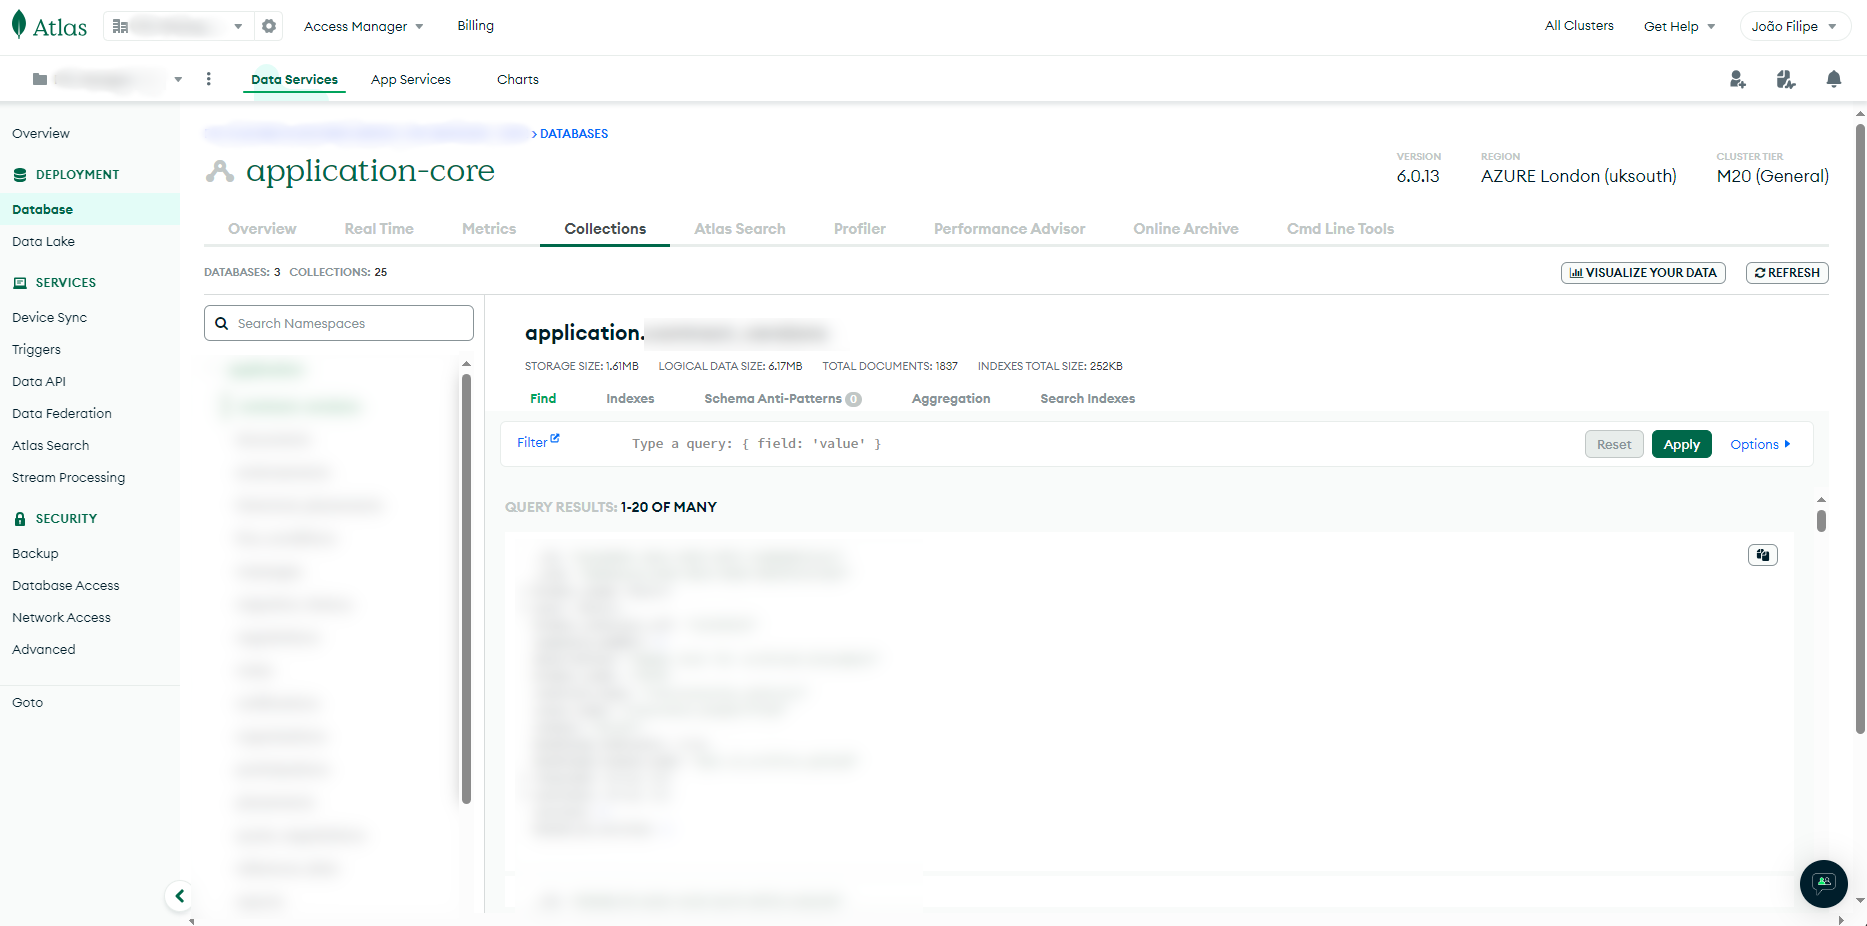
\includegraphics[width=\textwidth]{imgs/MongoDB.png} % You can replace 'example-image-a' with the path to your actual image
            \caption{Plataforma Atlas}\label{fig:atlas-ui}
            \source{Plataforma Interna do Atlas}
        \end{figure}

        Atlas, cuja interface se pode ver na Figura \ref{fig:atlas-ui}, é um componente crucial do processo, e é uma das plataformas mais usadas no que toca à resolução e análise de problemas.  
        
        A plataforma está integrada com todos os ambientes do projeto, permitindo escolher entre estes no canto superior esquerdo. Existem, no entanto, algumas restrições, por exemplo, para se poder ter acesso ao ambiente de produção, é necessário aceder primeiro à \hyperref[sec:plataforma-azure]{Plataforma Azure}, aceder a ``My roles'' > ``Groups'' e Pedir acesso com um campo para mencionar o número do Incidente em produção que vai ser analisado e uma pequena descrição.

        Um dos campos mais usados na plataforma é o dos filtros, visível na Figura \ref{fig:atlas-ui} onde é possível filtrar por campos específicos, organizar por data, colocando no campo ``sort'' por exemplo \texttt{\{``\_metadata.modified\_date'': -1\}} ou usar ``Aggregators'', na aba relacionada que permite a criação de pesquisas complexas passo a passo, removendo alguma dessa complexidade.

        É também aqui onde se gerem algumas das permissões relacionadas com a Base de Dados, ações reservadas apenas a alguns profissionais por questões de segurança. 
            
        \subsubsection{Competidores}\label{competidores-atlas}

            Em vez de uma base de dados NoSQL, a plataforma poderia beneficiar de uma base de dados SQL, até devido à melhor integração com outras ferramentas e à maturidade do mercado.

            Pelo que uma das alternativas a baixo tratadas é uma base de dados SQL.

            \subsubsubsection{Cosmos DB}\label{cosmos-db}

                Visto que é parte do ambiente Azure que já é extensivamente utilizado, seria mais fácil integrar com o projeto. Isto não quer dizer que uma transição seria fácil, normalmente transições deste tipo têm que ser muito bem justificadas devido aos preços e mão de obra exigidos.

                A escolha entre Cosmos DB e MongoDB depende das necessidades específicas da empresa. Cosmos DB destaca-se quando se necessita de flexibilidade com múltiplos modelos de dados, enquanto que o MongoDB se concentra no modelo de documentos. Cosmos DB oferece escalabilidade global e replicação automática em várias regiões, tornando-se ideal para baixa latência e elevada disponibilidade\cite{cosmosdb-vs-mongodb}.

            \subsubsubsection{MariaDB}\label{amazon-web-services}

                Esta seria uma solução que manteria um paradigma NoSql como o MongoDB. 

                MariaDB, uma base de dados relacional, adota o formato de tabela testado pelo tempo. Cada tabela no MariaDB segue um esquema fixo, definindo meticulosamente as colunas e os respetivos dados. Esta forma metódica de armazenar dados não apenas garante precisão, mas também estabelece estruturas predefinidas, fomentando clareza e organização o que contrasta com a utilização mais relaxada de BSON para armazenar dados em MongoDB.

    \subsection{Plataforma Azure}\label{sec:plataforma-azure}

        \begin{figure}[htbp]
            \centering
            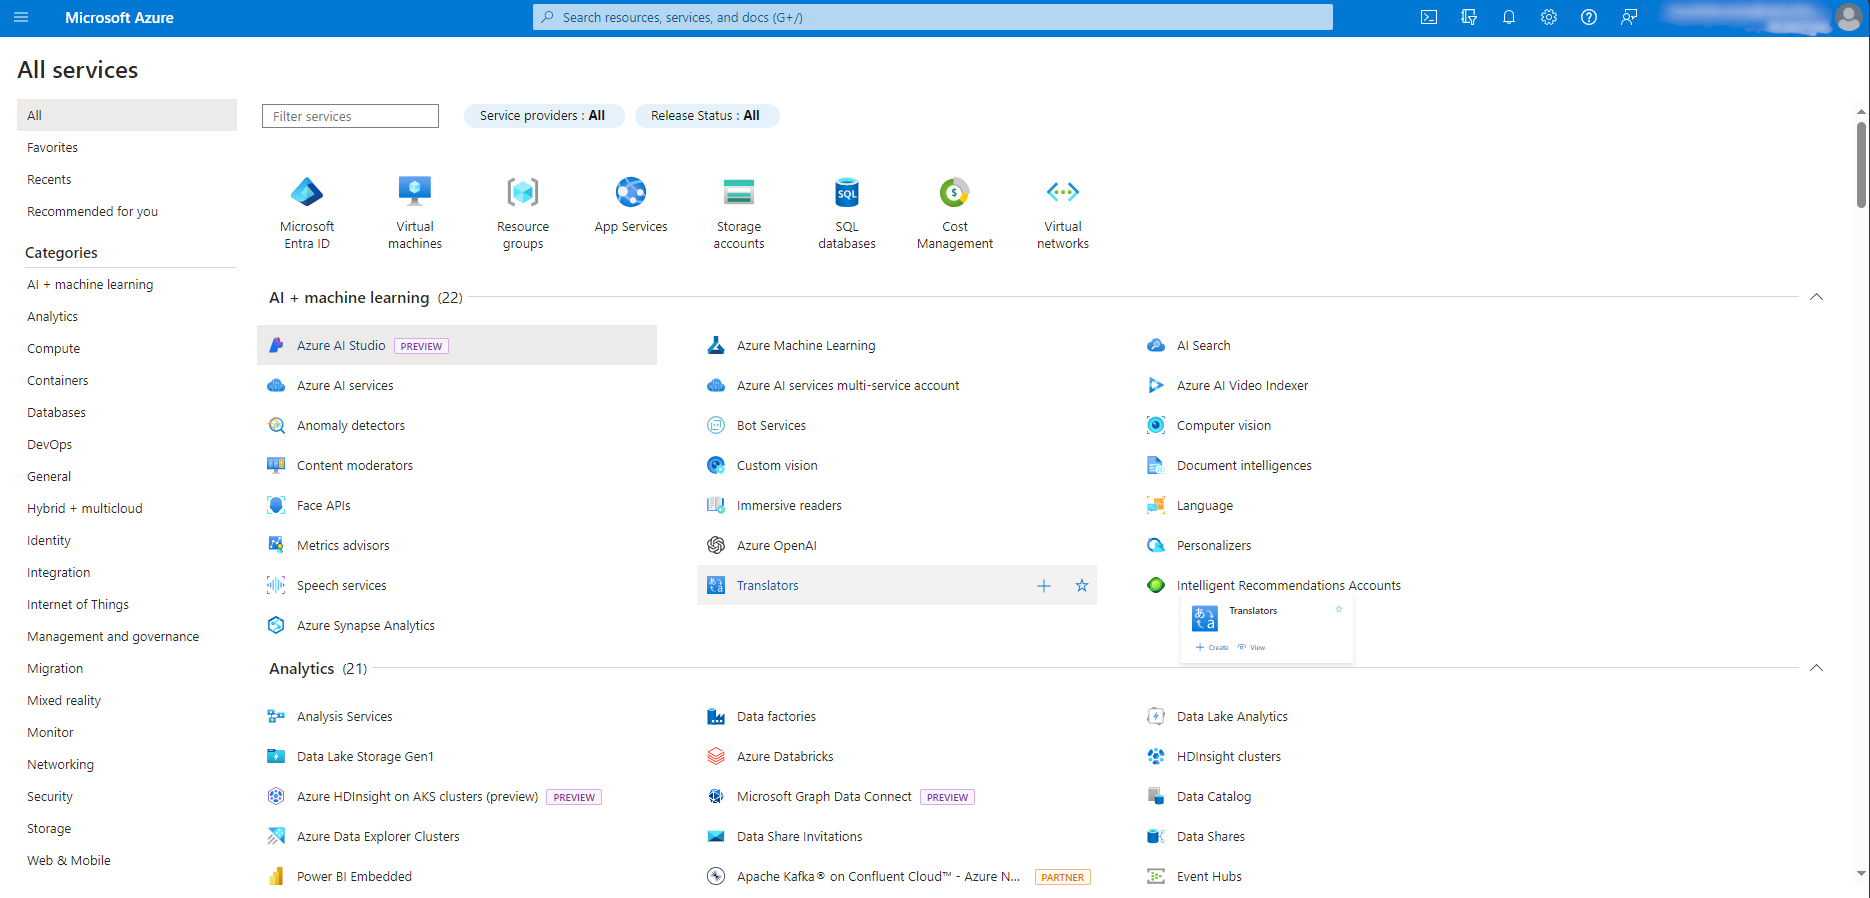
\includegraphics[width=\textwidth]{imgs/Azure.png}
            \caption{Plataforma Azure}\label{fig:azure-ui}
            \source{Plataforma Interna Azure}
        \end{figure}

        A plataforma Azure é a que engloba mais operações e áreas distintas do projeto, desde segurança até à gestão das máquinas virtuais usadas para os ambientes.

        Existe uma panóplia enorme de serviços, como é visivel na Figura \ref{fig:azure-ui}, estes incluem ``logic apps'', ``azure storage'', ``storage accounts'', ``Azure Virtual Network'' e ``Azure Health'', etc. Alguns dos que são mais usados e geridos na plataforma são os seguintes:

        \subsubsection{Resource Groups}

            Os \textit{Resource Groups} desempenham um papel crucial na organização e gestão eficiente dos recursos. Permitem agrupar recursos relacionados, como recursos de certos ambientes. Ao utilizar estes grupos, a administração torna-se também mais fácil e permite políticas de segurança e controlo de acessos a grupos específicos. 

        \subsubsection{Virtual Machines}

            É na gestão de Máquinas Virtuais do Azure que é possível aplicar os conceitos de \textit{scale out} e \textit{scale up} discutidos na Secção \ref{secsec:azure}, muitas vezes necessário para fazer um \textit{deployment} específico ou devido a fluxos invulgares de utilizadores para a plataforma. É nesta secção que se monitoriza o seu desempenho, se aplicam atualizações e se configuram as definições necessárias.

        \subsubsection{SQL Database} % perguntar ao Marcio o 

            A secção de SQL Database no Azure é essencial para a gestão e análise, manual ou automática, de bases de dados e outros problemas gerados pelas diferentes plataformas. É aqui que se tem acesso a todas as ferramentas avançadas do Azure para analisar os dados que podem ter vindo de qualquer ponto da plataforma.

        \subsubsection{Competidores}\label{competidores-azure}

            Devido à magnitude de serviços e funcionalidades que o Azure providencia, é difícil encontrar uma alternativa que disponha de todas as mesmas ferramentas, ou não tenha as suas próprias funcionalidades diferentes. Mas algumas ferramentas que podem ser consideradas são as seguintes:

            \subsubsubsection{Amazon Web Services(AWS)}\label{competidores-aws}

                O Amazon Web Services (AWS) é uma plataforma de nuvem também bastante usada no mercado, visto que a sua empresa mãe é a Amazon. Oferece uma ampla gama de serviços e soluções para atender às necessidades de organizações de todas as dimensões. Lançada em 2006, a AWS tornou-se rapidamente numa referência para o setor.

                A escolha entre Azure e AWS é depende muito das necessidades da empresa, por exemplo, uma empresa que precise de melhor integração com o Windows ou com PaaS, poderá estar melhor com o Azure, enquanto uma que necessite mais de IaaS, poderá estar melhor com a AWS.
                
                Ambas as ferramentas oferecem basicamente as mesmas funcionalidades, mas a AWS mantém-se a líder a termos de adoção global a 33\% enquanto o Azure se mantém apenas com 13\%\cite{aws-vs-azure}.

            \subsubsubsection{Oracle Cloud}\label{competidores-oraclecloud}

                A Oracle Cloud é também uma plataforma de nuvem proeminente no mercado, pertencente à Oracle Corporation e lançada em 2016\cite{launch-orcale-cloud}, incluindo serviços de computação, armazenamento, bases de dados (podendo servir também como alternativa ao Atlas), inteligência artificial, blockchain, etc. Também com um foco especial em aplicações empresariais.

                Tem um plano grátis que permite até acesso ilimitado a uma pequena máquina virtual, atraindo de início muitos pequenos negócios e empreendedores individuais.

                É também uma plataforma com serviços IaaS mais em foco, e mantém uma adoção de cerca de 8.43\%\cite{marketshare-oracle-cloud}.

    \subsection{Plataforma MS Teams}
    
        \begin{figure}[htbp]
            \centering
            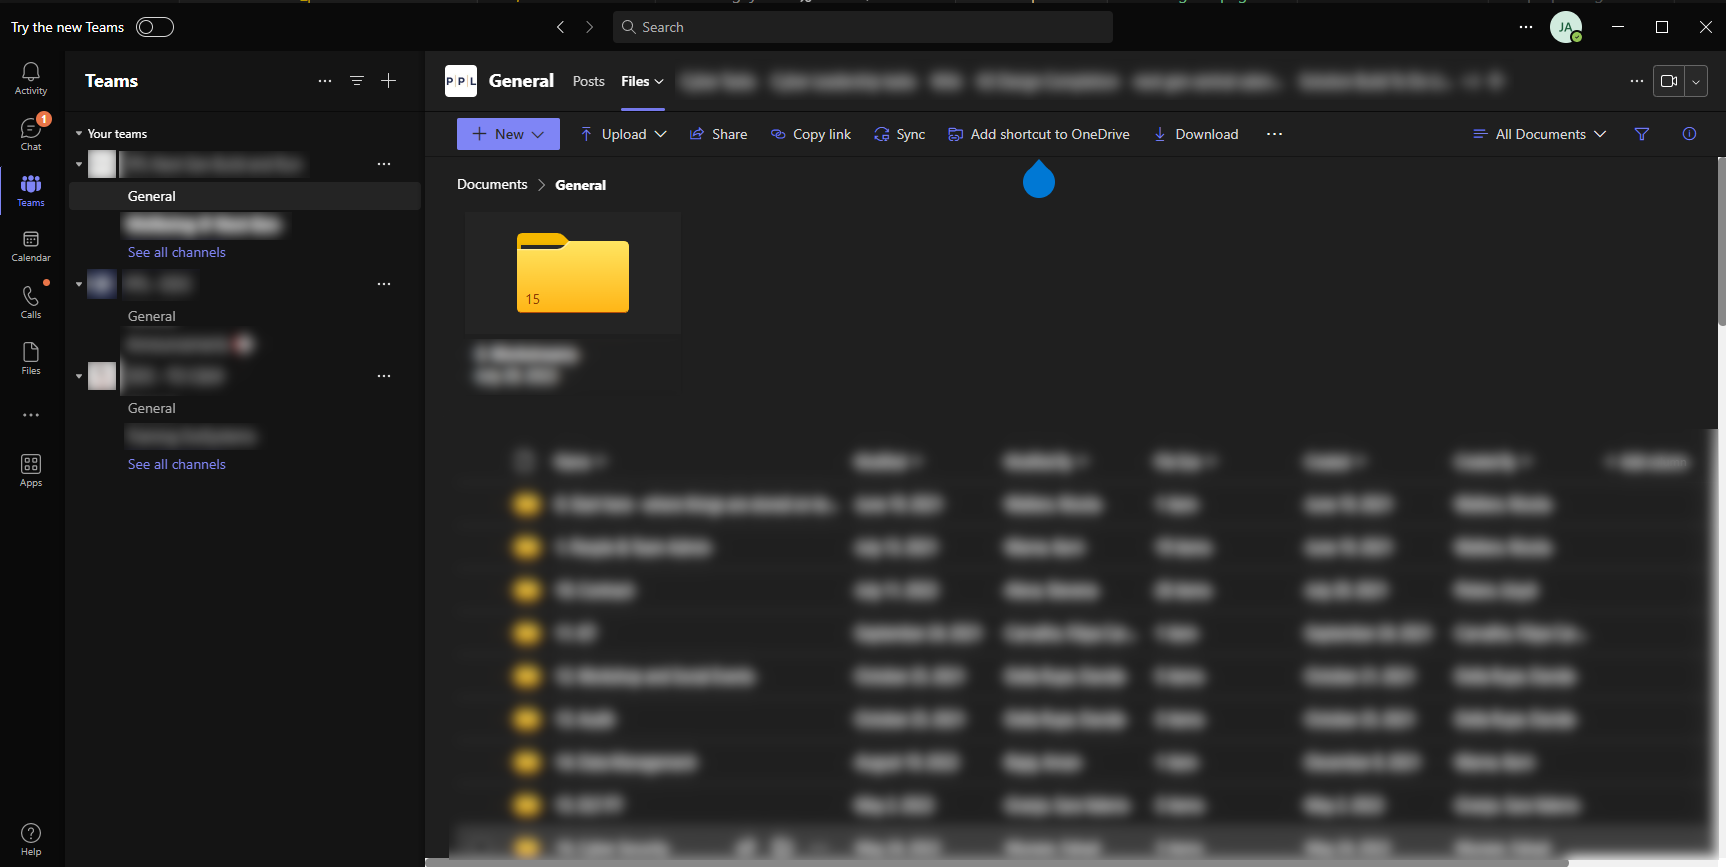
\includegraphics[width=\textwidth]{imgs/MSTeams.png} % You can replace 'example-image-a' with the path to your actual image
            \caption{Plataforma do Microsoft Teams}\label{fig:msteams-ui}
            \source{Plataforma Interna do Microsoft Teams}
        \end{figure}

        O Microsoft Teams é uma ferramenta essencial para a colaboração e comunicação eficaz na equipa. É onde acontece a maior parte da comunicação em tempo real por mensagens instantâneas, chamadas de áudio e vídeo, e colaboração em documentos em tempo real, tornando a componente geográfica transparente. É também onde se partilham muitos documentos e vídeos importantes para a organização do projeto, desde documentos Excel, como as férias de cada contratado, como vídeos gravados de formação dos KTs. Na Figura \ref{fig:msteams-ui} pode-se ver a página principal com as várias equipas de que um trabalhador faz parte à esquerda.
        %  (falados na secção \ref{sec:estrutura-organizacional-da-ril-na-deloitte-PT})
            
        \subsubsection{Competidores}\label{competidores-msteams}

        Visto que o MS Teams está intimamente integrado com muitas das ferramentas usadas diariamente, como o cliente de e-mail, Outlook, ou o calendário, ou SharePoint para partilha de ficheiros, é preciso considerar alternativas que ofereçam também estas ferramentas, ou permitam uma integração fácil com as mesmas.

            \subsubsubsection{Slack}\label{competidores-slack}

                O \href{https://slack.com/}{Slack} é uma plataforma de comunicação empresarial, permite a criação de canais para discussões específicas, integração com diversas ferramentas como calendários, permitindo que eventos sejam visualizados diretamente na plataforma. É possível partilhar documentos e ficheiros diretamente, mas não existe uma aba ou sítio onde se possam colocar ficheiros para todos os membros verem, para isto seria necessária uma solução de armazenamento externo como Google Drive ou SharePoint.
                
                Quanto aos preços, o Slack oferece uma versão gratuita com funcionalidades básicas e um histórico de mensagens limitado. As opções pagas, como o Slack Plus e o Slack Enterprise Grid, proporcionam funcionalidades avançadas, armazenamento adicional e suporte.

            \subsubsubsection{NextCloud Stack}\label{competidores-nextcloud}

                O \href{https://nextcloud.com/}{NextCloud} é a melhor alternativa no mercado de código aberto, oferece serviços como calendário, vídeo-chamadas, mensagens, listas \textit{to-do}, partilha de ficheiros, colaboração em ficheiros em tempo real, tudo isto em código aberto e livre de ser vetado, sendo uma boa alternativa para quem queira correr os próprios servidores, havendo também, no entanto, a possibilidade de pagar à empresa para usar os seus serviços na nuvem para correr a plataforma.

                Devido à natureza aberta da plataforma, existe uma comunidade vibrante que a rodeia, pelo que existem muitas extensões abertas feitas pela comunidade, havendo uma solução para quase qualquer funcionalidade que possa requerer, mas sendo estas funcionalidades desenvolvidas por indivíduos e não necessariamente equipas com um processo bem definido de desenvolvimento, podem muitas vezes não ser tão robustas como as funcionalidades base da plataforma.

    \subsection{Jira \& Confluence}\label{fuck_confluence_jira}

        Jira e Confluence são as ferramentas padrão da indústria para gestão de projetos ágeis e documentação colaborativa, respetivamente. A sua popularidade advém não apenas da sua robustez e fiabilidade, mas também da forma como se complementam, em parte por serem ambas desenvolvidas pela mesma companhia, Atlassian, oferecendo uma abordagem holística para o desenvolvimento de software e colaboração em equipa.

        Atlassian foi inicialmente fundada em 2002 por Mike Cannon-Brookes e Scott Farquhar como uma empresa que oferecia suporte a outras empresas, mas o software para gestão dos incidentes e defeitos usado na altura não era muito promissor, pelo que desenvolveram a sua própria ferramenta: JIRA. Criaram também um modelo de negócio para o desenvolvimento e venda desta ferramenta e, mais tarde em 2004, desenvolveram também o Confluence\cite{20-years-atlassian}.

        % Parágrafo sobre a Integração entre Jira e Confluence
        A integração entre Jira e Confluence forma uma poderosa sinergia, esta integração é notável em algumas funcionalidades como: ser possível adicionar incidentes da Jira diretamente na documentação do Confluence que são atualizados automaticamente, criar uma página do Confluence diretamente a partir das páginas da Jira, adicionar o estado de projetos da Jira no Confluence através de dashboards ou templates, ou adicionar novos incidentes diretamente através do Confluence ao sublinhar texto. 

        \subsubsection{Plataforma Jira}\label{secsec:jira}

            \begin{figure}[htbp]
                \centering
                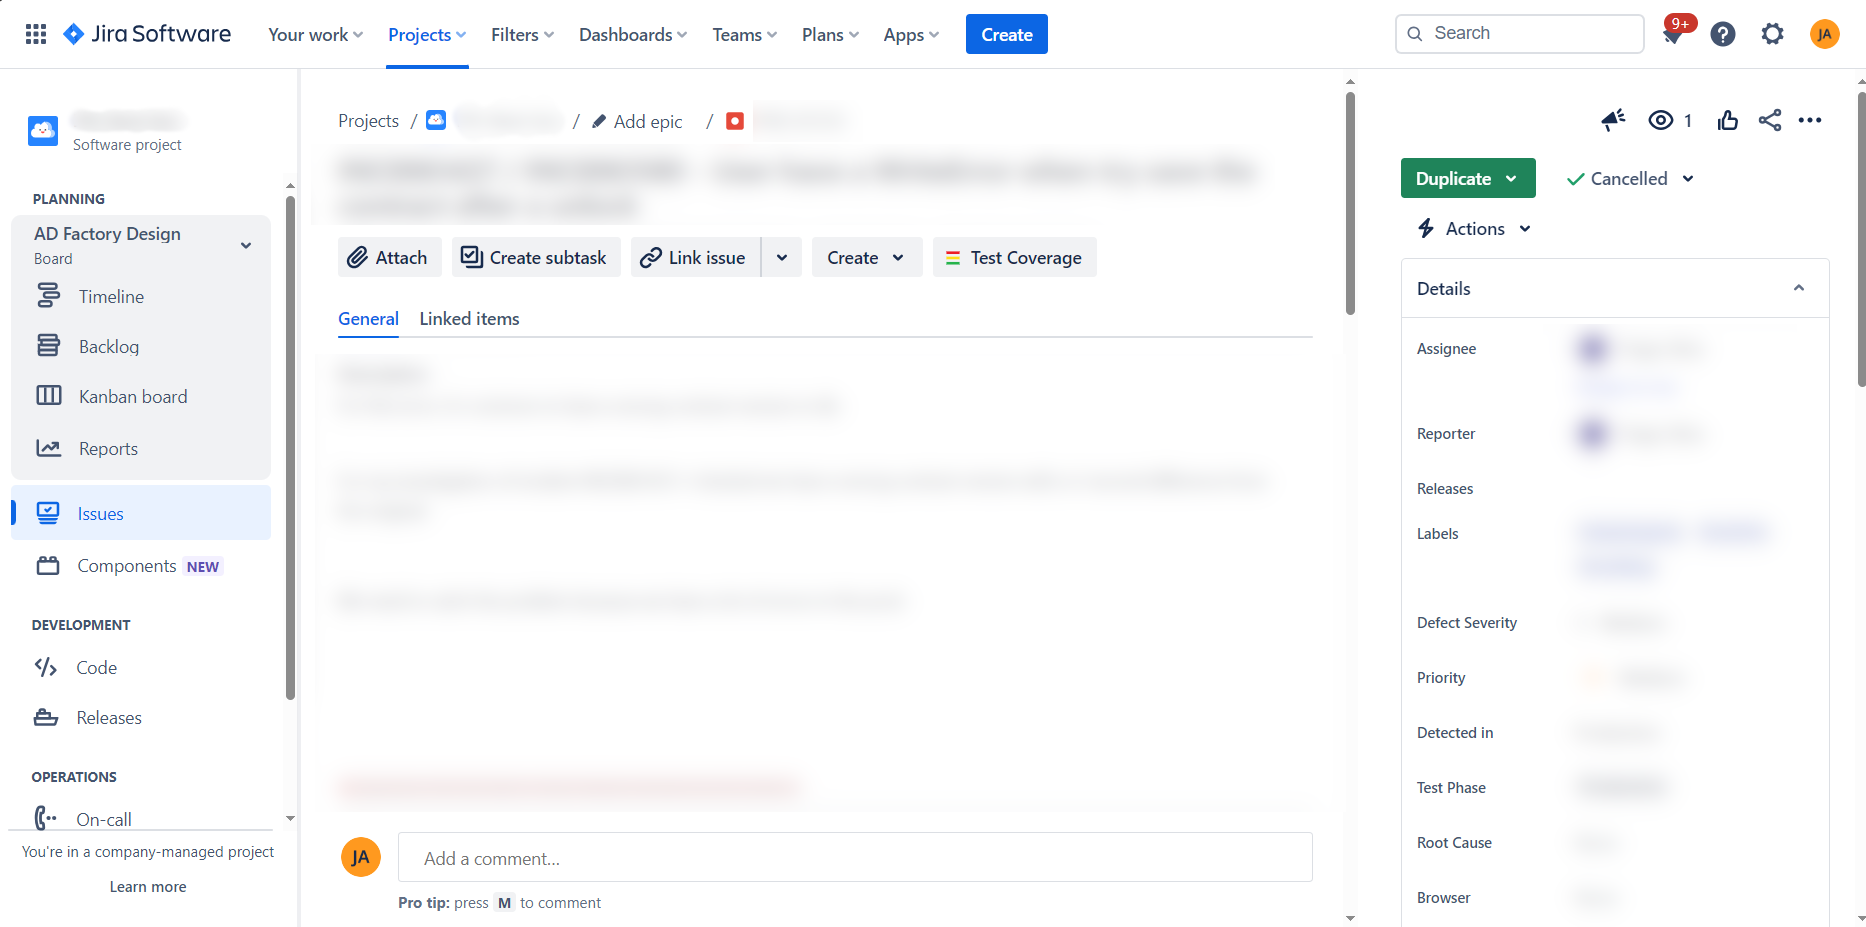
\includegraphics[width=\textwidth]{imgs/JiraSoftware.png} 
                \caption{Plataforma Jira Software}\label{fig:jira-ui}
                \source{Plataforma Interna da Jira}
            \end{figure}

            % Parágrafo sobre Jira
            A Jira facilita o desenvolvimento em metodologias ágeis, e é muito usada no projeto para manter um registo dos \textit{defects} existentes e em que estado se encontram, cada um identificado por um ID específico \textit{PNG-<XXXX>}, juntamente com o ID do incidente de que provieram se tiver sido esse o caso: \textit{INC-XXXXXX}. Existe um fluxo de estados, mostrado na Figura \ref{fig:defect-workflow}, pelo qual cada \textit{defect} tem que passar, começando no estado \textit{New} e acabando em \textit{Closed}, \textit{Duplicate} ou \textit{Rejected}. Na Figura \ref{fig:jira-ui} é possível ver interface da plataforma para a visualização de um \textit{defect}.

            \begin{figure}[htbp]
                \centering
                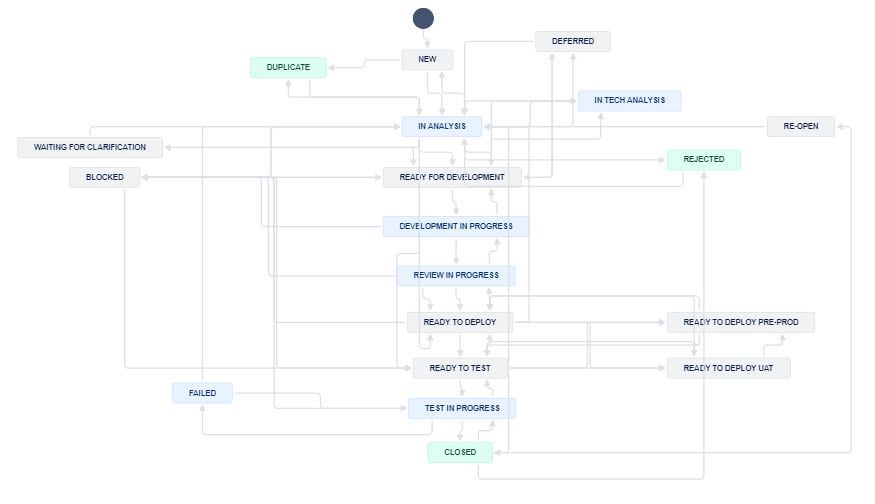
\includegraphics[width=\textwidth]{imgs/NextGenDefectWorkflow.png}
                \caption{RIL Next Gen \textit{Defect} workflow}\label{fig:defect-workflow}
                \source{Plataforma da Jira Interna}
            \end{figure}

            Em cada \textit{defect} pode-se também adicionar uma lista de \textit{subtasks} a qual necessita de ser completar, muitas vezes designados a diferentes membros da equipa ou até de equipas diferentes, por exemplo: \textit{Merge} do código para um ambiente específico, revisão do código, ou cenários de teste a executar. Cada \textit{subtask} tem também o seu próprio fluxo, como mostrado na Figura \ref{fig:ril-nextgen-subtasks-workflow}, começando em \textit{New} e podendo acabar em \textit{Complete} ou \textit{Cancelled}.

            \begin{figure}[htbp]
                \centering
                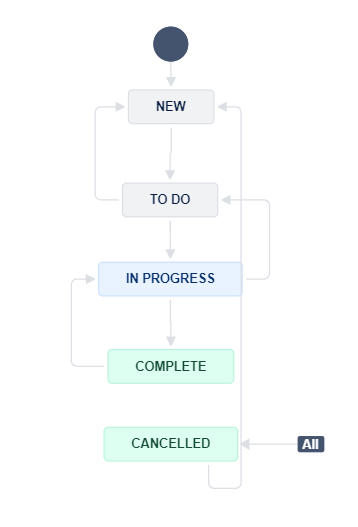
\includegraphics[scale=1.6]{imgs/NextGenSubTaskWorkflow.png}
                \caption{RIL Next Gen SubTasks workflow}\label{fig:ril-nextgen-subtasks-workflow}
                \source{Plataforma da Jira Interna}
            \end{figure}

            É possível também associar outros \textit{defects} na secção \textit{Linked Issues}, e qualquer colaborador pode deixar comentários e mencionar outros colaboradores, que irão subsequentemente receber um e-mail de aviso, permitindo fomentar um ambiente de forte e rápida comunicação.

        \subsubsection{Plataforma Confluence}\label{secsec:confluence}

            O Confluence é uma plataforma colaborativa de documentação e é onde a maior parte das descrições dos processos e complexidades está documentada, a sua interface é observável na Figura \ref{fig:confluence-ui}. Gere tudo desde os utiliza
            ores de teste que se podem utilizar nos diferentes ambientes e as suas credenciais, a incidentes ou \textit{defects} que ocorrem frequentemente bem como as suas resoluções, até à documentação de como realizar certas tarefas na aplicação ou numa das plataformas de desenvolvimento.
            
            \begin{figure}[htbp]
                \centering
                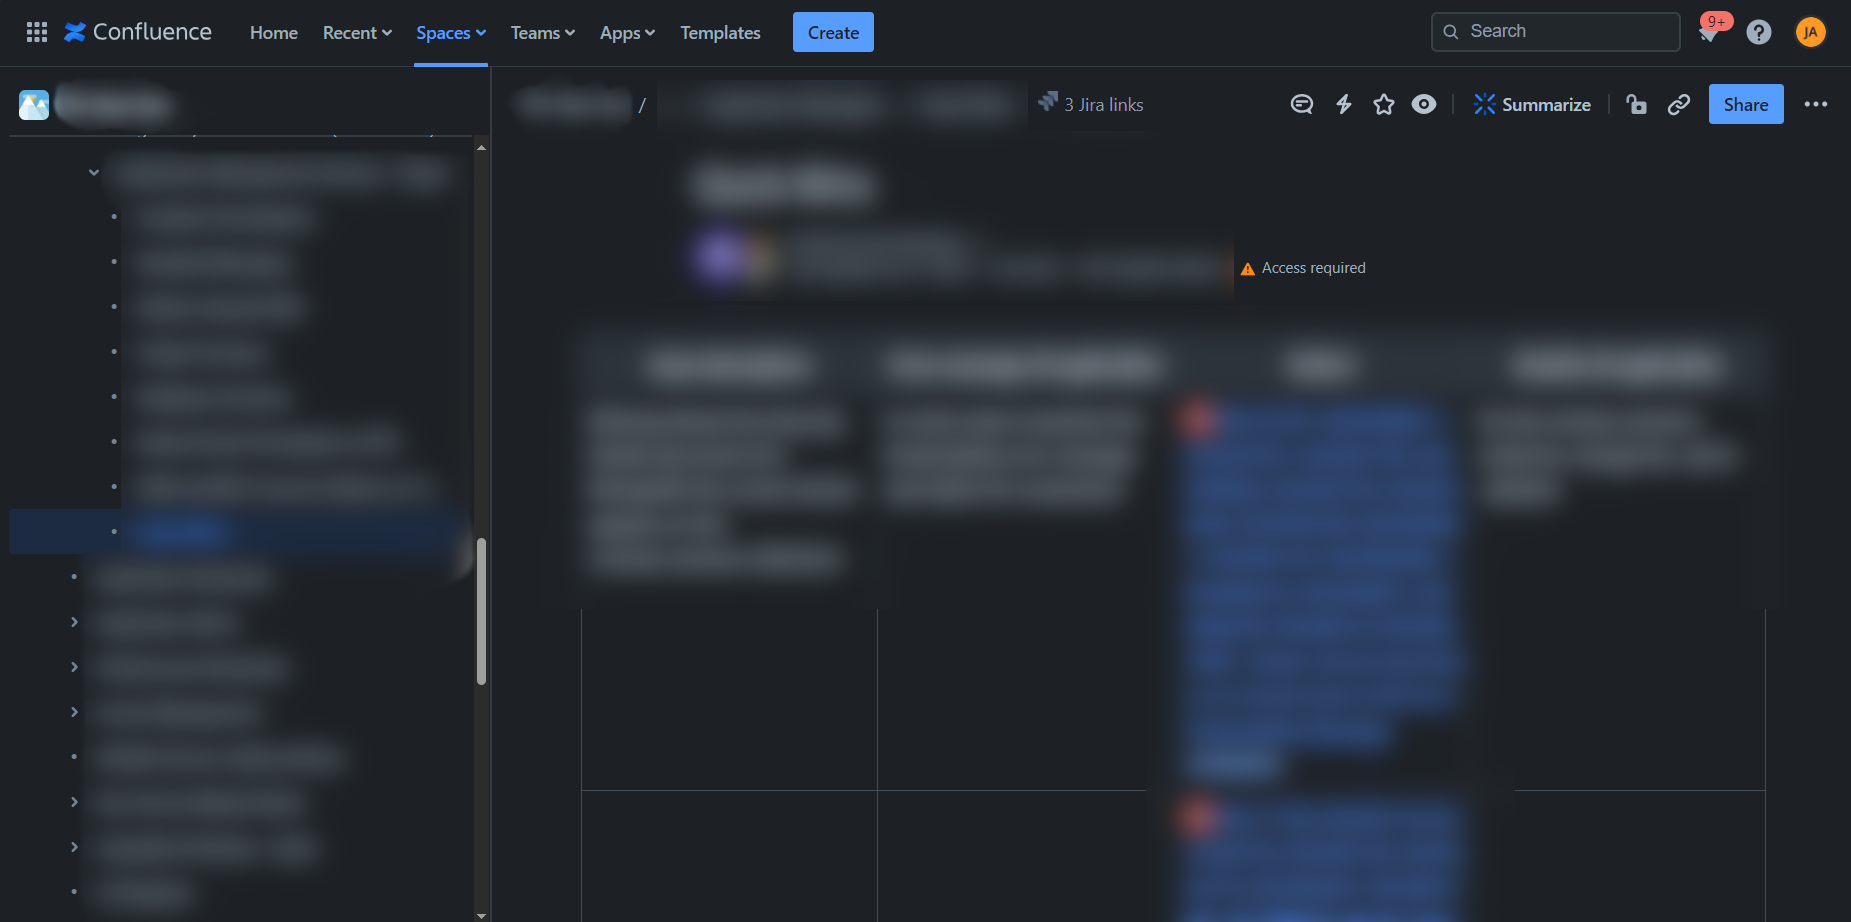
\includegraphics[width=\textwidth]{imgs/Confluence.png}
                \caption{Plataforma do Confluence}\label{fig:confluence-ui}
                \source{Plataforma do Confluence Interna}
            \end{figure}

            % Falar da agile board?
        
        \subsubsection{Competidores}\label{competidores-jira-confluence}

            Apesar de a Jira e do Confluence serem muitas vezes as ferramentas mais indicadas para a gestão de projetos, o preço destas pode ser um fator que leve a considerar outras ferramentas semelhantes, pelo que nesta secção vamos explorar algumas alternativas que possam substituir a junção do Confluence e da Jira.

        % https://www.reddit.com/r/devops/comments/10ksowi/alternative_to_atlassian_jira_and_confluence/

            \subsubsubsection{Linear + Notion}\label{linear-notion}

                \href{https://www.notion.so/}{Notion} é uma plataforma de colaboração e documentação com uma abordagem flexível e bastante personalizável mantendo uma interface simples e fácil de utilizar, permite a criação de páginas interativas, listas de tarefas, tabelas, integração com outras ferramentas como calendários e neste caso, \href{https://linear.app/}{Linear}. Esta última é uma ferramenta para desenvolvimento de software com foco no desempenho e precisão dos processos com funcionalidades como \textit{issue tracking}, listas e \textit{boards} e \textit{cycles}, uma funcionalidade que permite saber sempre qual é a tarefa em que se deve focar de seguida.
                
            \subsubsubsection{ClickUp}\label{clickup}
            
                \href{https://clickup.com/}{Clickup} é uma solução que engloba documentação e gestão de incidentes simultaneamente, é uma ferramenta que não teve tanto tempo ainda para se solidificar no mercado, mesmo em termos de integrações com outras ferramentas, mas é uma opção viável para equipas mais pequenas que procurem uma ferramenta mais simples e com um preço de entrada menor\cite{clickup-vs-jira}.

            \subsubsubsection{Bookstack + OpenProject}\label{bookstack}
            
                A alternativa de código aberto para equipas que querem garantir que o código que correm é seguro ou ter a possibilidade de contribuir diretamente ao projeto no caso de faltar alguma funcionalidade importante. Não existe, no entanto, nenhuma integração direta entre ambas as ferramentas.
                
                O \href{https://www.bookstackapp.com/}{Bookstack} é uma ferramenta de gestão de documentação que se destaca pela sua simplicidade e facilidade de uso. Oferece uma abordagem estruturada para a criação e organização de documentos.

                Já o \href{https://www.openproject.org/}{OpenProject} é uma plataforma de gestão de projetos de código aberto que oferece uma abordagem abrangente para planear, colaborar e acompanhar o progresso de projetos, permitindo uma gestão eficiente e transparente de tarefas, incidentes e equipas.
      
  \section{Tarefas no Âmbito do Projeto RIL}\label{sec:def_e_inc}

    Devido à natureza rotativa da equipa, foram efetuadas várias tarefas no âmbito do projeto. Nesta secção vamos analisar alguns dos testes, \textit{defects}, incidentes bem como outras tarefas que tenham sido concretizadas no contexto do estágio académico. Devido ao vasto número de incidentes e defeitos explorados e à natureza efémera da análise destes, visto que frequentemente a análise seria rodada para outra pessoa e ao curto tempo de análise, foi escolhida uma abordagem onde se vai analisar a fundo apenas algumas das tarefas, de forma a se detalhar bastante o processo.

    A participação do presente estagiário no projeto inicia-se em simultâneo com colega, que já colaborava com a Deloitte mas que era estranho ao projeto. Assim aproveitou-se para ambos aprenderem acerca das ferramentas e da lógica juntos em todas as circunstâncias em que tal fazia sentido.

    Como procedimento de acolhimento a recém-chegados, há uma fase inicial, após as formações iniciais mencionadas na Secção \ref{formacoes_introdutorias_empresa_cliente}, onde novos membros acompanhavam outros membros da equipa nas suas tarefas, como, por exemplo, as tarefas que acompanhavam dependiam das tarefas que estariam a ser realizadas na altura. Com tempo, passariam a fazer estas tarefas individualmente.

    \subsection{Resolver \textit{Defects}}\label{sub:defects}

        Nesta secção vão-se explorar alguns dos \textit{defects} resolvidos durante o período do estágio a fundo, incluindo ferramentas e métodos de trabalho e análise utilizados. Este método foi escolhido de forma ao leitor poder ficar com uma ideia clara do que é necessário e importante no processo do trabalho levado, desta forma uma análise profunda pode ser executada sem ser necessário fazê-la para todas as tarefas trabalhadas. Para uma visão holística do trabalho, a Tabela \ref{defeitos_trabalhados} detalha todos os defeitos trabalhados, respetivas prioridades de cada um.
        
        \begin{table}[htbp] % htbp
            \centering
            \begin{tblr}{
                % example for tblr: https://tex.stackexchange.com/questions/603349/tabularray-and-new-command-for-multicolumn-cells
                % another example: https://tex.stackexchange.com/questions/605676/tabularray-how-to-control-the-vertical-alignment-of-the-cells-contents
                hlines={lightgray}, vlines={lightgray},
                width = \linewidth,% total width set to width available
                %rows = {c,m}, % c aligns horizontally, m aligns vertically, aligns all rows
                colspec={X[3,c,m] X[3.5,c,m] X[c,m] X[c,m] X[1.2,c,m]},
            }
            % \textbf{Tempo trabalhado}
            \textbf{Título do \textit{defect}} & \textbf{Descrição do \textit{defect}} & \textbf{Prioridade} \\

            % Low, Medium, High, Critical

            ``A Withdrawn FO showing 'Requested' in overview screen \& 'Invalid Data' error message appearing when clicked on 'Requested''' & Um \textit{broker}, ao receber um FO, e esta ser retirada de seguida, o \textit{broker} consegue visualizar ``requested'' na tab ``overview'' para alguns dos UWs. Quando o \textit{broker} clica no estado ``requested'', surge uma mensagem de erro ``Invalid Data''. & Low \\

            ``The broker can't find the contract using the filter despite the UMR contract is showing in the filter that exists.'' & Contratos não conseguiam ser encontrados através dos filtros de procura. & Medium \\

            ``Regression - Subjectivity email notifications - Wrong emails getting triggered for subjectivity flow'' & Quando o UW apaga uma \textit{subjectivity} com o estado de ``satisfaction pending'', a subjetividade passa para o estado ``Proposed Deletion''. E quando o Broker aceita a proposta de exclusão da \textit{subjectivity}, o e-mail/notificação ``Firm Order - Update'' é acionado em vez do e-mail/notificação ``Subjectivity Deleted''. & Medium \\

            ``Amend Master Facility - UW not visible at Overview tab and Sign and Close page'' & O UW não se encontra visível na tab \textit{Overview} quando se efetuava uma alteração à MF. & Medium \\

            ``PRE - Master Facility - Post Bind Reference or Risk code changes are not showing any stamp details in the transaction logs'' & Ao criar um novo contrato, em certas situações, detalhes dos \textit{stamps} não eram criados. Não foi possível reproduzir. & Medium \\

            ``Stamp Visibility | Broker - The UW stamps should be filtered by the company.'' & Refira à Secção \ref{visibilidade_de_stamp_defect} & Medium \\

            ``Index out of bounds when submiting cancel and replace'' & Refira à Secção \ref{index_out_of_bounds_defect} & Urgent \\
            \end{tblr}
            \caption{Comparação de Plataformas Low-Code}
            \label{defeitos_trabalhados}
            \source{Documentação Interna} % 1- https://impalaintech.com/blog/mendix-vs-outsystems-vs-appian/
        \end{table}

        Vamos, primeiramente, detalhar a forma de análise de \textit{defects}:

        \subsubsection{Análise de \textit{Defects}}\label{secsec:analise_de_defects}

            De uma forma geral, os passos na análise e resolução de um \textit{defect} devem seguir os seguintes pontos:

            \begin{enumerate}
                \item A análise começa pela reflexão se o \textit{defect} está contemplado, ou não, nas USs, ou seja, se não será um GAP;
                
                Sendo um GAP, é passado à equipa relevante para a US ser alterada, caso contrário avança-se para o próximo passo: 
                \item De seguida deve-se identificar o ambiente em que se deve testar e resolver o \textit{defect};
                
                Existe um campo ``Target Fix Release'' que indica a release em que o \textit{defect} deverá ser resolvido, esta informação deve ser ligada ao deployment aggregator para identificar em qual dos ambientes de desenvolvimento se deve prosseguir, no caso dos ambientes do protótipo da Figura \ref{fig:deployment-aggregator}, os ambientes DED ou DES.  
                \item Deve-se então atualizar o ``Assignee'' para o nosso utilizador na plataforma;
                \item Analisar, preparar e corrigir o \textit{defect} na plataforma Service Studio atualizando sempre o estado no \textit{defect} apropriadamente, neste caso de \textit{New} para \textit{In Analysis} para \textit{Ready For Development} conforme o flow demonstrado na Figura \ref{fig:defect-workflow};
                \item De seguida o mais apropriado será alinhar com os maestros. Para tal será necessário realizar testes e revisões do código e possivelmente retrofit para um ambiente mais a baixo, são também criadas ``subtasks'' para estas tarefas que são, no entanto,  frequentemente realizadas por outras equipas. 
            \end{enumerate}

        \subsubsection{Índice fora dos limites ao submeter \textit{Cancel and Replace}}\label{index_out_of_bounds_defect}

        \textit{Defect} original: ``\textit{Index out of bounds when submiting cancel and replace}''

            % ``defect com a liliana'' no onenote

            Um dos primeiros \textit{defects} analisados, foi analisado em conjunto com um membro da equipa numa dinâmica de \textit{Remote Pair Programming}.

            \textbf{\textit{Pair Programming}}: Também conhecido por \textit{peer programming}, é um estilo de programação ágil onde dois programadores trabalham em conjunto no mesmo dispositivo no mesmo problema\cite{peer-programming}, existe debate àcerca do método e da sua eficácia mas tem sido observado sendo benéfico em casos onde a tarefa é complexa e uma alta precisão no código é essencial, ou tarefas simples onde o tempo é limitado, sendo também uma boa forma de aprendizagem e integração, onde participantes reportam resultados positivos em áreas como a aprendizagem, confiança no código, tempo necessário e gosto geral no processo\cite{faja2014evaluating,hannay2009effectiveness}. % \parencites{faja2014evaluating}{hannay2009effectiveness}. 

            \begin{table}[htbp] % 
                \centering
                \begin{tabularx}{1\textwidth}{|>{\raggedright\arraybackslash}X|}
                    \hline
                    \rowcolor{lightgray}
                    \textbf{\textit{Defect}} \\
                    \hline
                    \rowcolor{lightgray!20}
                  
                    \begin{quote}
                        \textbf{Descrição do Defeito:}

                        Ao fazer uma correção do tipo \textit{Cancel and Replace}, quando o \textit{broker} submetia a correção ao \textit{underwriter}, aparecia o erro: ``Index out of bounds. Index -1 for bounds [0,0]''.
                        
                        \begin{itemize}
                            \item Resultado Atual: Ocorre o erro: ``Index out of bounds. Index -1 for bounds [0,0]'';

                            \item Resultado Esperado: O \textit{broker} deve ser capaz de enviar a correção ao \textit{underwriter} sem erros;

                            \item Possível Continuar com o Fluxo: Não;

                            \item Solução Alternativa: Não há;

                            \item Passos para Reproduzir:
                            \begin{itemize}
                                \item Criar um \textit{placement} com 1 \textit{underwriter};

                                \item Enviar um pedido de Firm Order;

                                \item Aceitar o pedido de Firm Order;

                                \item O \textit{broker} cria uma correção do tipo \textit{Cancel and Replace};

                                \item Não fazer alterações pelo \textit{Cancel and Replace};

                                \item Submeter o pedido pressionando ``Send Correction to Underwriter'';

                                \item Ao seguir estes passos, o erro ``Índice fora dos limites. Índice -1 para limites [0, 0]'' deve ser exibido.
                            \end{itemize}
                        \end{itemize}
                    \end{quote}

                    \\
                    \hline
                \end{tabularx}
                \caption{Detalhes do defeito '\textit{Index out of bounds when submitting cancel and replace}'}\label{table:defect1}
                \source{Documentação Interna}
              \end{table}

            \subsubsubsection*{Análise e Resolução:}

                A descrição do \textit{defect} em causa encontra-se na Tabela \ref{table:defect1}. Fazendo a análise segundo a Secção \ref{secsec:analise_de_defects}:

                \begin{enumerate}
                    \item Neste caso, visto que o \textit{defect} se referia a um erro de limites que aparecia na própria plataforma, não foi necessário procurar a US referente à funcionalidade, isto porque facilmente se deduz ser um comportamento causado por um erro no código que não é desejado na lógica de negócio;

                    \item Nesta etapa foram feitos testes que demonstraram que o erro se encontrava apenas em um dos ambientes de desenvolvimento, pelo que se procedeu a analisar e resolver o defeito neste ambiente;

                    \item Já se tinha atualizado o ``Assignee'';

                    \item A fase de análise e correção é sempre a mais demorada e imprevisível, sempre atualizando o estado do defeito quando apropriado:
                    
                    O processo de desenvolvimento e resolução está muito dependente da comunicação com os membros mais adequados da equipa para cada etapa, pelo que grande parte da capacidade de resolução de problemas, especialmente numa fase inicial, depende muito de uma capacidade de comunicação com os colegas de trabalho. 

                    A análise começou com uma troca de informação com uma BA familiarizada com o flow de \textit{cancel and replace} que nos direcionou para a ação com a lista onde provavelmente ocorria o problema.

                    De seguida fomos à ação em causa, ativamos o debugger do Service Studio, fizemos um \textit{cancel and replace} na plataforma e identificamos a causa do problema, como é possível ver na Figura \ref{fig:index_out_of_bounds1}, o ID do contrato chegava vazio à lista. 

                    \begin{figure}[H]
                        \centering
                        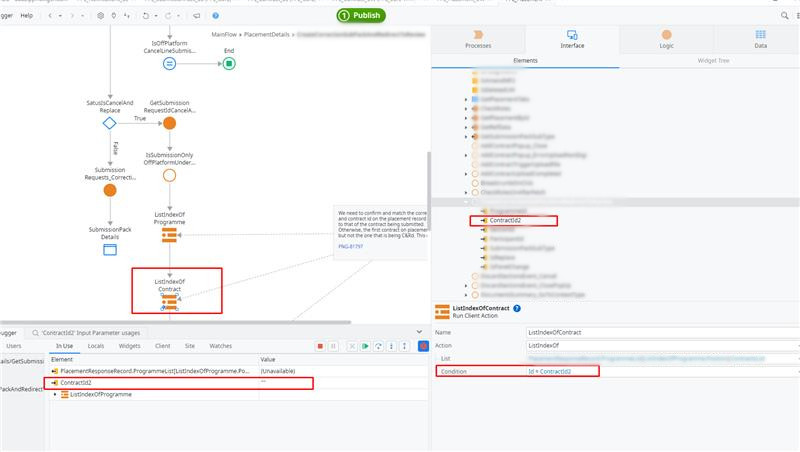
\includegraphics[width=\textwidth]{imgs/IndexOutOfBounds1.jpg}
                        \caption{Index Out of Bounds - Root of the Problem}\label{fig:index_out_of_bounds1}
                        \source{Service Studio Interno}
                    \end{figure}

                    Analisou-se então a interface e de onde vinha o ID do contrato inicialmente ao pressionar o botão, e descobriu-se que o ID era passado ao bloco corretamente. Portanto, era no meio da comunicação, desde quando se clicava no botão até à ação em questão, que se perdia o valor.

                    Os dados eram passados quase exclusivamente de blocos para blocos a partir de \textit{block events}.

                    \textbf{Blocos em OutSystems}: É uma interface reutilizável com código, widgets, ou outros blocos \cite{os-blocks}.

                    \textbf{Eventos de Blocos}: São eventos que permitem ao bloco interagir com o parente do bloco. Estes eventos podem ter variáveis de input ou de output, visto que o ecrã ou o bloco pai não sabe se algo acontece no bloco, como um botão ser clicado, usam-se eventos para passar esta informação para fora, que podem também ser de caráter obrigatório\cite{os-block-events}.

                    Havia uma passagem da informação entre 4 blocos, cujos eventos chamavam diretamente outros eventos, sem haver oportunidade de colocar \textit{breakpoints} no meio do fluxo, depois de uma troca entre um colega acerca do funcionamento de \textit{triggers} em OutSystems, procedeu-se à criação de ações auxiliares que apenas chamavam eventos, e fez-se com que os eventos chamassem estas ações. Desta forma já era possível colocar \textit{breakpoints} e descobrir em que passagem se perdiam os dados. 
                    
                    Veio-se a descobrir que na passagem onde se perdiam os dados, o nome da variável de onde vinham os dados de um bloco era igual ao nome da variável para onde iam os dados noutro bloco, isto normalmente não seria um problema, mas, OS, com o seu código interno em C\#, tem dificuldades em fazer um registo e passagem correta de dados em caso de nomes iguais, pelo que se procedeu à mudança do nome e à publicação da aplicação, o que acabou por solucionar o problema.
                    
                    Retiraram-se então as ações auxiliares e atualizou-se o estado do \textit{defect} adequadamente;
                    
                    \item Nesta etapa comunicou-se com o nosso líder de equipa, e foi necessário reverter as mudanças. O leitor pode ter-se apercebido que o segundo ponto não seguia o padrão de análise de \textit{defects} estabelecido na Secção \ref{secsec:analise_de_defects}. Era necessário analisar o deployment aggregator e não apenas resolver o defeito no ambiente de desenvolvimento em que este ocorria. 
                    
                    Veio-se a descobrir que durante aquele período o código de ambas as plataformas de desenvolvimento deveria ser idêntico dado que o código de uma iria substituir a outra brevemente. Pelo que a resolução foi revertida e a análise foi guardada apenas como informação no \textit{defect}, que mais tarde foi usada por um colega que aplicou a resolução na altura e no ambiente correto.
                \end{enumerate}

        \subsubsection{Visibilidade de stamp | Corretora — Os stamps de UW devem ser filtrados pela empresa}\label{visibilidade_de_stamp_defect}

        \textit{Defect} original: ``\textit{Stamp Visibility | Broker - The UW stamps should be filtered by the company}''

            \begin{table}[htbp] % htbp
                \centering
                \begin{tabularx}{1\textwidth}{|>{\raggedright\arraybackslash}X|}
                    \hline
                    \rowcolor{lightgray}
                    \textbf{\textit{Defect}} \\
                    \hline
                    \rowcolor{lightgray!20}
                  
                    \begin{quote}
                        \textbf{Descrição do Defeito:}
                    
                        Um \textit{broker} cria um novo contrato, depois de preencher todas as informações obrigatórias e carregar o documento MRC (documento obrigatório para contratos), seleciona um UW que participará no contrato.
    
                        Se selecionar um UW A (Empresa X), que pertence a várias equipas dentro da Empresa X e Empresa Y (ambas as empresas estão sob a mesma organização), quando seleciona ``Permitted Territory'' - ``Show All'', só devo ver todos os stamps que o UW A tem atribuídos na Empresa X, mas vê-se os stamps atribuídos na Empresa X e Y.
    
                        \begin{itemize}
                            \item Passos para Reproduzir:
                                \begin{itemize}
                                    \item Criar um contrato;
                                    \item Selecionar um UW que pertence a 2 ou mais empresas da mesma organização;
                                    \item Selecionar ``Show All'' no território permitido;
                                    \item Validar se os stamps disponíveis para o \textit{broker} são os stamps atribuídos ao UW dentro dessa empresa.
                                \end{itemize}
                        \end{itemize}
                    \end{quote}

                    \\
                    \hline
                \end{tabularx}
                \caption{Detalhes do defeito '\textit{Stamp Visibility | Broker - The UW stamps should be filtered by the company}'}\label{table:defect2}
                \source{Documentação Interna}
            \end{table}
            
            \subsubsubsection*{Análise e Resolução:}

                A descrição do \textit{defect} encontra-se na Tabela \ref{table:defect2}. Começou-se a análise pela verificação da US associada à funcionalidade, depois de uma troca com um membro da equipa familiarizado com as USs, identificou-se a US da Tabela \ref{table:us1}.

                \begin{table}[H] % htbp
                    \centering
                    \begin{tabularx}{1\textwidth}{|>{\raggedright\arraybackslash}X|}
                        \hline
                        \rowcolor{lightgray}
                        \textbf{User Story:} Lista de stamps --- Adicionar um stamp \\
                        \hline
                        \rowcolor{lightgray!20}
                      
                        \begin{quote}
                            \textbf{Visão da User Story:} Para a configuração de um Transportador, os stamps estão vinculados à hierarquia (Organização, Empresa e Utilizador). Esta US permitirá a criação de uma lista de stamps. A lista de stamps também incluirá a ocultação de stamps inativos na lista global.
                        
                            \textbf{Como...} Administrador RIL
                        
                            \textbf{Eu quero...} Adicionar um stamp
                        
                            \textbf{Para quê...} Configurar uma lista de stamps
                        
                            \textbf{Critérios de Aceitação de Negócios:}
                        
                            \textbf{Configuração inicial do ecrã de stamps:}

                            \begin{itemize}
                                \item Dado o Administrador RIL estar no ecrã ``hierarquia'' \newline
                                Quando o Administrador RIL seleciona a aba ``stamps'' \newline
                                Então, a descrição da aba será ``lista de stamps'';

                                \item Dado o Administrador RIL estar na tela ``hierarquia'' \newline
                                Quando o Administrador RIL seleciona a aba ``stamps'' \newline
                                Então, mostra as seguintes colunas de dados (na ordem listada): Nome do stamp, tipo de agência, tipo de stamp, válido a partir de, válido até, estado, classificação e ação;

                                \item Dado o Administrador RIL estar no ecrã ``hierarquia'' \newline
                                Quando o Administrador RIL seleciona a aba ``stamps'' \newline
                                Então, por defeito, mostrar uma lista de carimbos ATIVOS para a organização;
                            
                                \item \textit{etc.}
                            \end{itemize}
                            
                        \end{quote}
                        \\
                        \hline
                    \end{tabularx}
                    \caption{Detalhes da US ``\textit{List of Stamps - Add a Stamp}''}\label{table:us1}
                    \source{Documentação Interna}
                \end{table}

                Após a análise desta US, deduziu-se que se tratava de um GAP, isto porque na US original dizia ``por defeito, mostrar uma lista de carimbos ATIVOS para a organização'', não implicando que devam ser filtrados por empresa, filtragem esta que não se faz na aplicação, e isso torna-se evidente neste caso em que o utilizador pertence a várias equipas em diferentes empresas na mesma organização.

                Foi então reportado no próprio \textit{defect} e notificadas as equipas relevantes, que continuaram com o problema a partir daí.

            % Outro defect Defect [PNG-74147] Stamp Visibility | Broker - The UW stamps should be filtered by the company. - Jira (atlassian.net)

    \subsection{Reportar \textit{Defects}}\label{sub:reportar_defects}

        Pode acontecer que através de testes, ou incidentes, ou mesmo apenas usando a plataforma, se depare com um erro ou comportamento inesperado, o qual pode ter que ser reportado como defeito. Circunstância esta que aconteceu ao presente estagiário quando conseguiu carregar dois documentos MRC para apenas um contrato, algo que não devia ser possível. 
        
        Ocorria também, com alguma frequência, membros da equipa descobrirem defeitos durante o apoio a testes. Como parte do seu trabalho cabia-lhes, mediante solicitação,  
        ajudar a documentá-los e a registá-los na plataforma Jira.

        O processo de reportar defeitos é bastante intuitivo e envolve a criação de uma entrada no Jira, onde são fornecidos detalhes essenciais para a compreensão e resolução do problema. Este processo implica frequentemente a confirmação com membros da equipa sobre campos cruciais, como a versão principal, tipo de defeito, data de deteção, fase de teste, \textit{sprint}, versão afetada, severidade e prioridade.

        Detalhes adicionais, como descrição, passos para reproduzir o defeito, se o utilizador fica ou não bloqueado, qual a solução alternativa, resultado esperado e resultado atual, são também incluídos no registo do defeito. Este nível de detalhe facilita a triagem, análise e resolução eficaz por parte da equipa de desenvolvimento futuramente.

        % tipo o de adicionar vários contratos a um documento: 

        % Podes filtrar no Jira por reported by me

    \subsection{Análise de Incidentes}\label{sub:incidentes}

        Incidentes, ao contrário de \textit{defects}, têm uma certa urgência associada, devido a serem um problema reportado diretamente por um utilizador, havendo, normalmente, alguém à espera que este seja resolvido. Pelo que se recorre muito mais a \textit{datafixes} para desbloquear utilizadores e nem sempre é possível ou viável chegar à causa, ou raiz dos problemas.

        % ``O meu primeiro Incident'' No onenote INC0063053

        \subsubsection{INC0064225 - Todas as seleções são inválidas}\label{secsec:inc0064225} % INC0064225 com o marcio

            Incidente original: ``\textit{All selections invalid}''

            % OMG INCIDENTE INC0064225, aquele que fizeste datafix com o marcio

            \begin{table}[H] % htbp
                \centering
                \begin{tabularx}{1\textwidth}{|>{\raggedright\arraybackslash}X|}
                    \hline
                    \rowcolor{lightgray}
                    \textbf{Incidente INC0064225} \\
                    \hline
                    \rowcolor{lightgray!20}
                  
                    \textbf{Descrição do Incidente:} O utilizador ficou bloqueado ao submeter uma nova Firm Order. Depois de fazer o processo todo de submissão como esperado, aparecia o erro ``All selections are invlaid, Please review the breakdown below and select Cancel to return to the Submission Pack'', apresentando por baixo uma lista com todos os UWs a dizer estarem inativos.

                    \\
                    \hline
                \end{tabularx}
                \caption{Incidente INC0064225}\label{table:usincINC0064225}
                \source{Resumo da Informação do Incidente no Service Now}
            \end{table}

            A descrição do incidente encontra-se na Tabela \ref{table:usincINC0064225}.

            Durante a investigação, verificou-se um possível equívoco no número fornecido pelo utilizador ``NM0011234'', que se presumiu que deveria ser ``NM0011224''. 

            Identificou-se inicialmente a possibilidade de resolver o problema removendo e adicionando novamente a \textit{Master Facility} à declaração. Esta abordagem foi sugerida ao utilizador, como uma solução potencial para o problema.
            
            Ao analisar as participações associadas à \textit{Facility}, notou-se ainda uma discrepância numa delas, relacionada com um utilizador chamado ``John''. Embora não pareça ser a causa direta do problema, esta discrepância foi registada para investigação adicional, caso a solução inicial não fosse bem-sucedida.

            Foi então mandado o pedido ao utilizador para adicionar a MF de novo. Recebeu-se resposta negativa atempadamente, informando-nos que isto já fora tentado e não funcionara.
            
            No entanto, na base de dados era possível ver que a última mudança ao contrato fora à mais de uma semana atrás, foi decidido, portanto, fazer a \textit{datafix} para corrigir o utilizador ``John'' e marcar uma reunião com o utilizador. Devido ao tempo que o \textit{datafix} levou a ser aplicado, acabou por não se conseguir falar com o utilizador antes do final da semana. Mas mais tarde recebeu-se a notícia que o \textit{datafix} efetuado fora suficiente para desbloquear o utilizador e o incidente pôde ser fechado.
            
        \subsubsection{INC0065686 - Não foi possível enviar o cancelamento}\label{secsec:inc0065686} % INC0064225 com a ines
                
            Incidente original: ``\textit{Unable to submit cancelation}''

            \begin{table}[H] % htbp
                \centering
                \begin{tabularx}{1\textwidth}{|>{\raggedright\arraybackslash}X|}
                    \hline
                    \rowcolor{lightgray}
                    \textbf{Incidente INC0065686} \\
                    \hline
                    \rowcolor{lightgray!20}
                
                    \textbf{Descrição do Incidente:} O utilizador mandou uma Firm Order para um UW que não devia ter mandado, por isso clicou em ``withdraw'' do pedido, mas o UW conseguiu aceitar. Ao ver que o UW tinha aceite, foi mandado um pedido de cancelamento, mas o UW não conseguia visualizá-lo, e ao abrir a submissão deste pedido, o programa fica parado a carregar infinitamente.

                    \\
                    \hline
                \end{tabularx}
                \caption{Incidente INC0065686}\label{table:incINC0065686}
                \source{Resumo da Informação do Incidente no Service Now}
            \end{table}

            A descrição do incidente encontra-se na Tabela \ref{table:incINC0065686}.

            No decorrer da análise do incidente INC0065686, foi identificado o problema na base de dados. Existe uma sequência de documentos criados na DB de MongoDB que são criados quando o estado de um UW é mudado, estas são as negotiations. Depois de se comunicar com um membro da equipa familiarizado com o funcionamento desta coleção, apercebeu-se que depois da negotiation com o estado ``withdrawn'' foi gerada subsequentemente uma negotiation com o estado \texttt{pending\_unconditional\_line}, que significa que o pedido tinha sido enviado para o UW mesmo tendo sido withdrawn; se fosse um novo pedido e não o mesmo, teria que haver uma negotiation \texttt{request\_for\_line\_or\_binder} antes da \texttt{pending\_unconditional\_line}.

            Não foi encontrada nenhuma indicação na Base de Dados do pedido de cancelamento descrito pelo utilizador.

            Depois de alguma discussão decidiu-se que a solução seria fazer um ``soft delete'' das negociations depois do withdraw. Para manter a integridade da base de dados foi necessário também alterar a coleção das ``participations'', que continha informação àcerca do UW e da sua participação atual no contrato, tendo sido necessário remover cinco campos que tinham sido inadvertidamente adicionados devido às negotiations erróneas que foram criadas, e alterado o campo status da participation para ``new''.
            
            No fim foi criado um \textit{defect} com os passos para reproduzir por definir onde se detalhou o problema: ``UW capaz de aceitar pedido withdrawn''.

            % INC INC0065686 (aquele que viste com a inês e foi preciso mandar datafix para remover as negotiations)

            % Incidente do Craveiro no onenote
            %  aquele que falaste com o user com a andereia, e que o problema era os subpanels

    \subsection{Testes}\label{sub:tests}

        Durante o período de estágio, as responsabilidades incluíam a realização de testes sempre que solicitado pela equipa. O processo de teste envolvia uma abordagem sistemática para garantir a o funcionameninto e integridade adequados das funcionalidades desenvolvidas, e pode-se dividir nos seguintes passos:
        
        \begin{itemize}
            \item \textbf{Recebimento da Solicitações de Teste:} Ao ser solicitado, forma-se uma compreensão dos requisitos e casos a testar. Como por exemplo a identificação do ambiente a testar, e recolha de quaisquer documentos que possam ser necessários;
            \item \textbf{Recriação das condições do Teste:} Criação das condições na plataforma para recriar o teste com base nas especificações fornecidas;
            \item \textbf{Execução de Testes:} Interação com a aplicação, seguindo as especificações do teste, recolhendo evidências videográficas se necessário;
            \item \textbf{Registo de Resultados:} Documentação dos resultados, por exemplo, no defeito em caso, incluindo comportamentos inesperados e evidências;
            \item \textbf{Comunicação com a Equipa:} Segue-se o relato conciso dos resultados obtidos com quem os solicitou.
        \end{itemize}

        A principal destreza necessária para realizar estes testes é uma boa perceção da lógica de negócio e da plataforma. Os seguintes são alguns exemplos de testes feitos durante a duração do estágio:

        \begin{itemize}
            % Um da bárbara sobre a proposed line não ser revertida
            \item Criação de um contrato com duas secções, ambas com uma mistura de UWs off e on platform e uma mistura de \textit{roles} entre eles, mandar e aceitar o contrato, fazer uma \textit{correction} do tipo ``panel change'' e alterar a percentagem proposta por cada UW sem \textit{roles} de 60\% para 50\%. Aceitá-las \textit{section} 1 e rejeitá-las na \textit{section} 2, no \textit{section} rejeitada, deveria voltar a 50\% | 50\% proposed, em vez de 50\% | 60\%. O comportamento esperado foi o observado pelo que não se replicou;
            % Outro da Bárbara(e agora que tens que ver o codigo) sobre os archive placements
            \item Carregar \textit{placements} arquivados a partir de uma folha Excel onde o \textit{placing broker} especificado pertencia a uma organização com duas companhias diferentes onde ambas tinham \textit{branches} com nomes idênticos. Isto fazia com que ao ir buscar o utilizador do Excel, este pudesse ser extraído do \textit{branch} errado, resultando no bloqueio do utilizador devido à plataforma considerar estes dados inválidos;
            % Um teste sobre Receber notificações: on cancelation
            \item Criar uma \textit{declaration} com um \textit{leader} e um \textit{follower}, nenhum dos UWs têm \textit{roles}, enviar e aceitar, selecionar ``cancel line'' na declaration e enviar. Notar que o \textit{follower} não recebeu notificação da \textit{cancelation};
            % Podes falar dos testes que a Inês te deu, por exemplo o dos endorsements
            \item O preenchimento de uma folha de Ecel acerca da informação presente no documento gerado pelos contratos e \textit{endorsements} dos contratos numa variedade de casos diferentes com UWs off e on platform.
        \end{itemize}

    \subsection{Análise de Processos}\label{sub:processos}

        Uma das tarefas delegadas ao presente estagiário foi também a análise de processos de OS. Dentro do Service center é possível analisar sob as abas ``Monitoring'' e ``Processes'' os processos da aplicação e como é que estes foram concluídos ou em que estado estão, na Figura \ref{fig:interface_processo_servicecenter} pode-se ver a interface da plataforma ao visualizar os detalhes de um processo.

        Os processos aqui analisados são processos que acabavam suspensos, muitas vezes bastante antigos. São processos que causariam problemas a utilizadores se estes interagissem com o contrato específico associado a este processo, frequentemente podiam ser recomeçados e continuariam normalmente, mas em muitas das situações isto não acontece, esta situação oferece a possibilidade de identificar problemas com a plataforma e possíveis erros a resolver.

        \begin{figure}[H]
            \centering
            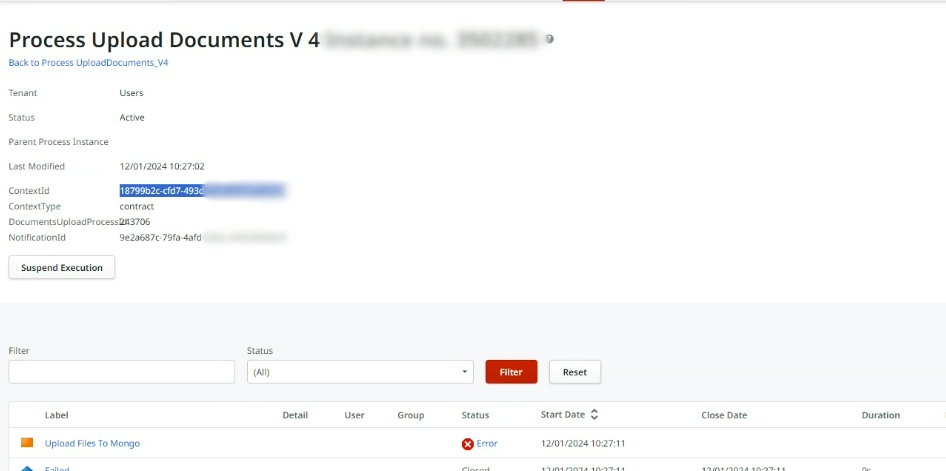
\includegraphics[width=\textwidth]{imgs/ProcessoServiceCenter.png}
            \caption{Interface de análise de um processo - Service Center}\label{fig:interface_processo_servicecenter}
            \source{Service Center Interno}
        \end{figure}

        Todos os processos revistos, independentemente do seu estado, tinham que ser anotados num documento de Excel específico para a tarefa com informação dos IDs dos contratos, \textit{placements}, equipas e utilizadores associados ao processo, bem como os erros ocorridos, caso tal seja relevante.

        Devido à natureza frequentemente repetitiva da análise destes, foi elaborado um web scraper em python que auxiliou na análise de alguns processos, por exemplo, foi automatizado o caso em que o processo \texttt{GenerateMRCEmailProcess} estava associado a um utilizador que estivesse inativo, registando e clicando ``skip'' na plataforma automáticamente, para mais informações refira à Secção \ref{secsec:scriptspython}.

        Existem três tipos de processos que geravam erros e era preciso analisar:

        \subsubsection{\texttt{SDC\_Generation}}\label{secsec:sdc_generation}

            % Isto é por causa da equipa de SDC para não sobrecarregarem

            Possivelmente o mais difícil de se analisar dos processos aqui representados.
            
            Foi imposto um limite de 10 processos recomeçados com sucesso por hora e 50 por dia, de forma a não sobrecarregar a equipa dos processos.

            OS erros levantados neles tinham origem nos stamps das negociações e das suas complexidades. Devido à sua natureza volátil, e a criarem \textit{roles} diferentes para utilizadores e terem uma lógica de pertença a utilizadores e organizações pouco intuitiva, a sua ocorrência dependia de várias contingências.

            Em cada processo analisado era necessário encontrar a negociação e os stamps associados e fazer uma análise do campo \texttt{sdc\_enable} de cada stamp. Caso houvesse pelo menos um com a valor lógico verdadeiro para este campo, tentava-se correr de novo o processo, caso contrário, registava-se e não se tentava correr.
             
            Os processos podiam acabar numa das seguintes formas:
            \begin{itemize}
                \item \textbf{Closed}: Quando o processo correu de novo e concluiu com sucesso;
                \item \textbf{Error}: Quando acontecia um erro na execução, o erro era extraído e registado atempadamente;
                \item \textbf{Active --- Loop}: Quando fica num estado cíclico, por vezes durante horas. Na maior parte destes casos os processos acabariam por ficar suspensos de novo.
            \end{itemize}

        \subsubsection{\texttt{GenerateMRCEmailProcess}}\label{secsec:generate_mrc_email_process}

            Os processos \texttt{GenerateMRCEmailProcess} envolvidos na geração dos documentos MRC (\textit{Mutual Responsibility Contract}). O erro mais recorrente neste processo era identificado pela mensagem ``There was a technical issue sending the notification to the user <ID>''. Após uma análise detalhada do fluxo de ações nos logs do Azure, identificou-se que este problema ocorre quando uma ação tenta aceder a um documento na base de dados que não tem o campo URI preenchido, indicando a falta da referência ao documento na plataforma Nuxeo. A solução recomendada, caso um utilizador se depare e reporte o problema, é solicitar ao utilizador que execute a ação ``cancel and replace''.

            Outro erro detetado seria o identificado pela mensagem ``Invalid Username and password''. Neste caso, era feita uma validação para verificar se o utilizador estava inativo na base de dados. Se estivesse, era pressionado o botão ``skip'' no processo, pois não havia ações adicionais a serem tomadas. Caso o utilizador estivesse ativo, a informação era anotada e o estado atual era mantido. Eventualmente, poder-se-ia verificar nos logs do Azure as ações executadas até ocorrer o erro para identificar a ação que o causou.

            % Erro mais comum: There was a technical issue sending the notification to the user <ID>
            % Depois de revisto o fluxo de ações chamadas nos logs do azure, foi possível perceber que o erro ocorre quando uma ação chama um documento que na base de dados não tem o uri preenchido, ou seja não tem referenncia ao documneto.
            %A solução se um user se queixar seria pedir são utilizador para fazer cancel and replace.

            % Tinham outro erro: Invalid Username and password, e aqui é que faziamos a validação de se o user está inativo ou não: ver na Base de dados o utilizador, Se estiverem Inativos, ent davamos skip, não há nada a fazer, dar skip, Caso se encontre um ativo anota-se e deixa-se como está (ou eventualmente ver no azure os logs das ações percorridas até dar o erro).
        
        \subsubsection{\texttt{UploadDocuments\_V4}}\label{secsec:uploaddocuments_v4}

            O processo \texttt{UploadDocuments\_V4} desempenha um papel na gestão de documentos da plataforma, é na sequência de uma asserção da integridade destes documentos na plataforma, que surgiu a necessidade de fazer a análise destes processos. 
            
            O principal objetivo é validar se um documento está presente no Nuxeo e na base de dados do OutSystems em sincronia, utilizando o identificador do documento.

            O procedimento envolve a consulta à base de dados MongoDB para verificar se o campo URI do documento está preenchido, indicando a existência do documento no Nuxeo, e confirmando na plataforma. Se o documento estiver presente, prosseguia-se com o botão ``skip''. Caso contrário, se não existir informação na base de dados MongoDB, a situação seria registada. Nos casos em que o contrato associado ao documento também não é encontrado, a ação ``skip'' seria considerada. É relevante notar que durante a duração relevante, não foi registado nenhum cenário onde o contrato existia num \textit{placement} mesmo sem ter um URI.

            % O objetivo seria ver se o documento está presente no Nuxeo e em OutSystems
            % Viamos na base de dados o documento atravez do ID
            % Queremos ver se o campo uri está preenchido com qualquer coisa, que se tiver quer dizer que existe no Nuxeo. Mas para confirmar podiamos ir mesmo ao Nuxeo: Copiavas o Uri e punhas no nuxio e deve aparecer
            % Se aparecer, podes clicar no skip:
            % Se não aparecer nada na base de dados MongoDB, Anotavam no Excel e não lhe mexíamos. Mas antes disso, procuravas o contrato, se o contrato não existisse também, aí podiam dar skip: 
            % O caso em que o contrato existe nunca foi encontrado antes!

                \subsubsection{Scripts de Automação em Python}\label{secsec:scriptspython}

            Com o intuito de otimizar o processo e mediante as adequadas autorizações concedidas, o estagiário assumiu a responsabilidade de automatizar a análise dos processos. Foram consideradas diferentes opções de interação com os APIs internos do Azure, OutSystems e MongoDB. Contudo, para obter acesso programático à base de dados de produção, seria necessário solicitar aprovação diretamente ao cliente, à RIL. Além disso, os APIs feitos para o Azure de produção não tinham um histórico favorável de funcionamento em Python, existiam apenas programados em C\#.

            Diante a situação, optou-se por se automatizar através da implementação de um web scraper e da interação direta com o navegador. Os scripts criados estão disponíveis no Anexo \ref{sec:scripts}.

            \subsubsubsection{User Stories}\label{secsecsec:us_python}

                Realizou-se assim um estudo das User Stories (US) a implementar, com o objetivo de reduzir ao mínimo os requisitos, garantir uma implementação rápida e alcançar um elevado nível de automatização. Este processo conduziu à identificação das US das tabelas \ref{table:python_us1}, \ref{table:python_us2}, \ref{table:python_us3} e \ref{table:python_us4}.

                \begin{table}[htbp] % htbp
                    \centering
                    \begin{tabularx}{1\textwidth}{|>{\raggedright\arraybackslash}X|}
                        \hline
                        \rowcolor{lightgray}
                        \textbf{User Story:} Análise de Processos SDC no Estado ``Active - Loop'' \\
                        \hline
                        \rowcolor{lightgray!20}
                                        
                        \begin{itemize}
                            \item \textbf{Visão:} Efetuar uma análise detalhada dos dados dos processos SDC presentes num ficheiro Excel local, identificando aqueles que se encontram no estado "Active - Loop". Posteriormente, realizar uma avaliação dos dados do processo e dos erros associados. A tarefa inclui a atualização do estado para "Suspended" no Excel, juntamente com o registo do tipo de erro e a URL correspondente.

                            \item \textbf{Como...} Utilizador autorizado a executar operações sobre os processos SDC no estado "Active - Loop".

                            \item \textbf{Eu quero...} Analisar os dados dos processos SDC no estado "Active - Loop", corrigir os erros associados, atualizar o estado para "Suspended" no Excel e registar informações detalhadas sobre o tipo de erro e a URL no mesmo ficheiro.

                            \item \textbf{Para quê...} Garantir uma gestão eficaz dos processos SDC, corrigindo problemas associados e mantendo um registo claro das ações realizadas para futura referência e auditoria.
                        \end{itemize}
                        \\
                        \hline
                    \end{tabularx}
                    \caption{Detalhes da US \textit{Análise de Processos SDC no Estado ``Active - Loop''}}\label{table:python_us1}
                \end{table}

                \begin{table}[htbp] % htbp
                    \centering
                    \begin{tabularx}{1\textwidth}{|>{\raggedright\arraybackslash}X|}
                        \hline
                        \rowcolor{lightgray}
                        \textbf{User Story:} Análise de Processos GenerateMRCEmailProcess com Utilizadores Inativos \\
                        \hline
                        \rowcolor{lightgray!20}
                                        
                        \begin{itemize}
                            \item \textbf{Visão:} Efetuar uma análise dos dados dos processos \texttt{GenerateMRCEmailProcess}, contidos num ficheiro Excel local, focando-se nos processos que possuem apenas o número na primeira coluna, sem informações adicionais. Utilizando a plataforma Atlas, identificar os processos que apresentam o utilizador inativo e, automaticamente, pressionar o botão ``skip'' na plataforma Service Center para cada um deles. Preencher sempre com os dados do processo no Excel.

                            \item \textbf{Como...} Utilizador autorizado a realizar operações relacionadas com os processos \texttt{GenerateMRCEmailProcess} e a aceder à plataforma Atlas.

                            \item \textbf{Eu quero...} Analisar os dados dos processos \texttt{GenerateMRCEmailProcess} presentes no ficheiro Excel, identificar os processos com utilizadores inativos através do Atlas e automatizar a exclusão destes processos na plataforma Service Center.

                            \item \textbf{Para quê...} Assegurar uma gestão eficiente dos processos \texttt{GenerateMRCEmailProcess}, evitando a interação com utilizadores inativos e otimizando o fluxo de trabalho no Service Center.
                        \end{itemize}
                        \\
                        \hline
                    \end{tabularx}
                    \caption{Detalhes da US \textit{Análise de Processos GenerateMRCEmailProcess com Utilizadores Inativos}}\label{table:python_us2}
                \end{table}
                
                \begin{table}[htbp] % htbp
                    \centering
                    \begin{tabularx}{1\textwidth}{|>{\raggedright\arraybackslash}X|}
                        \hline
                        \rowcolor{lightgray}
                        \textbf{User Story:} Análise de Processos \texttt{UploadDocuments\_V4} no Excel \\
                        \hline
                        \rowcolor{lightgray!20}
                                        
                        \begin{itemize}
                            \item \textbf{Visão:} Efetuar uma análise dos dados dos processos \texttt{UploadDocuments\_V4} presentes num ficheiro Excel local. Verificar se o ``ContextI'' dos processos não tem nenhum documento associado na base de dados de Produção do MongoDB. Em caso negativo, assinalar no Excel com a mensagem ``Contract does not exist in Mongo'' e prosseguir. Se existir, verificar se todos os documentos possuem um URI e, em caso afirmativo, assinalar no Excel com o comentário ``Document in Mongo''. A informação será sempre registada no Excel.

                            \item \textbf{Como...} Utilizador habilitado a executar operações relacionadas com os processos \texttt{UploadDocuments\_V4} e a aceder à base de dados de Produção do MongoDB.

                            \item \textbf{Eu quero...} Analisar os dados dos processos \texttt{UploadDocuments\_V4} no ficheiro Excel, verificar a existência de documentos associados ao ``ContextId'' na BD do MongoDB e assinalar no Excel as mensagens adequadas conforme as condições verificadas.

                            \item \textbf{Para quê...} Assegurar uma gestão precisa dos processos \texttt{UploadDocuments\_V4}, identificando casos em que o contrato não existe na base de dados do MongoDB ou verificando se todos os documentos possuem um URI, proporcionando um registo claro e informado no Excel.
                        \end{itemize}
                        \\
                        \hline
                    \end{tabularx}
                    \caption{Detalhes da US \textit{Análise de Processos GenerateMRCEmailProcess com Utilizadores Inativos}}\label{table:python_us3}
                \end{table}

                \begin{table}[htbp] % htbp
                    \centering
                    \begin{tabularx}{1\textwidth}{|>{\raggedright\arraybackslash}X|}
                        \hline
                        \rowcolor{lightgray}
                        \textbf{User Story:} Interrupção Controlada da Execução do Script \\
                        \hline
                        \rowcolor{lightgray!20}
                                        
                        \begin{itemize}
                            \item \textbf{Visão:} Permitir a interrupção controlada da execução do script a qualquer momento através da combinação de teclas CTRL + ALT + S.

                            \item \textbf{Como...} Utilizador precisa de interromper a execução do script de forma controlada e imediata.

                            \item \textbf{Eu quero...} Ter a capacidade de interromper o script em execução em qualquer ponto utilizando a combinação de teclas \texttt{CTRL} + \texttt{ALT} + \texttt{S}.

                            \item \textbf{Para quê...} Proporcionar ao utilizador um meio eficiente de parar a execução do script quando necessário, garantindo uma interrupção rápida e controlada, sem comprometer a integridade dos dados ou funcionalidade do sistema.
                        \end{itemize}
                        \\
                        \hline
                    \end{tabularx}
                    \caption{Detalhes da US \textit{Análise de Processos GenerateMRCEmailProcess com Utilizadores Inativos}}\label{table:python_us4}
                \end{table}

            \subsubsubsection{Requisitos Funcionais}\label{secsecsec:req_func_python}

                A partir das USs, foram derivados os requisitos funcionais, apresentados na tabela \ref{tab:req_func_python}. Estes requisitos representam as descrições e comportamentos externos exigidos pelo software, delineando as funcionalidades que o sistema deve cumprir. Proporcionam uma visão de alto nível do sistema.
                
                \begin{table}[htbp] % htbp
                    \centering
                    \begin{tblr}{
                        % example for tblr: https://tex.stackexchange.com/questions/603349/tabularray-and-new-command-for-multicolumn-cells
                        % another example: https://tex.stackexchange.com/questions/605676/tabularray-how-to-control-the-vertical-alignment-of-the-cells-contents
                        hlines={lightgray}, vlines={lightgray},
                        width = \linewidth,% total width set to width available
                        %rows = {c,m}, % c aligns horizontally, m aligns vertically, aligns all rows
                        colspec={X[1,c,m] X[5,l,m]}, % the first number is the size
                    }
                    % \textbf{Tempo trabalhado}
                        \textbf{ \# } & \textbf{Nome} \\
                        REQ-01 & Análise de Processos SDC \\
                        REQ-02 & Análise de Utilizadores Inativos em GenerateMRCEmailProcess \\
                        REQ-03 & Análise de Documentos em UploadDocuments\_V4 \\
                        REQ-04 & Interrupção Controlada do Script \\
                        REQ-05 & Pintar Colunas com Erros de Roxo para Análise Manual \\
            
                    \end{tblr}
                    \caption{Requisitos funcionais dos scripts para análise de processos}
                    \label{tab:req_func_python}
                \end{table}

                Na tabela \ref{tab:req1_py} está representado, a título de exemplo, um requisito funcional, está acompanhado de um resumo detalhado e descrição. A lista completa dos requisitos encontra-se disponível no Anexo \ref{sec:Req_func_python_anexo}.

                \begin{table}[htbp] % htbp
                    \centering
                    \begin{tblr}{
                        % example for tblr: https://tex.stackexchange.com/questions/603349/tabularray-and-new-command-for-multicolumn-cells
                        % another example: https://tex.stackexchange.com/questions/605676/tabularray-how-to-control-the-vertical-alignment-of-the-cells-contents
                        hlines={lightgray}, vlines={lightgray},
                        width = \linewidth,% total width set to width available
                        %rows = {c,m}, % c/l/r aligns horizontally, m/t/b aligns vertically, aligns all rows
                        colspec={X[1,l,m] X[5,l,m]}, % the first number is the size % the second is c for center, l for left
                    }
                    % \textbf{Tempo trabalhado}
                        \textbf{ Nome } & \textbf{REQ-01 --- Análise de Processos SDC} \\
                        Resumo                  & Este requisito visa permitir a análise detalhada dos processos SDC num ficheiro Excel local, focando-se na identificação e correção dos processos no estado "Active - Loop". \\

                        Descrição               & O sistema deve possibilitar a identificação dos processos SDC no estado "Active - Loop" num ficheiro Excel local. Após a análise, o estado destes processos deve ser atualizado para "Suspended", e informações detalhadas sobre erros e URLs associadas devem ser registadas no Excel. \\

                        Requisitos Relacionados & -- \\
            
                    \end{tblr}
                    \caption{Requisito funcional \textit{Análise de Processos SDC}}
                    \label{tab:req1_py}
                \end{table}

                Devido à simplicidade deste projeto, requisitos não funcionais não foram apurados.
                
            \subsubsubsection{Implementação e Arquitetura}\label{secsecsec:implementacao_python}

                Seguidamente, procedeu-se à implementação de três scripts distintos para os três primeiros casos de uso. Desta forma, foi desenvolvido um script para analisar cada tipo de processo: um para a análise dos processos SDC já concluídos, outro para a análise dos processos MRC cujos utilizadores se encontravam inativos, e um terceiro para a análise global dos processos Documents\_V4. Para isto foram utilizadas diversas bibliotecas em Python, incluindo:

                \begin{itemize}
                    \item \texttt{json}: Utilizada para lidar com a manipulação de dados em formato JSON;

                    \item \texttt{pyautogui}: Esta biblioteca foi empregada para automatizar a interação com a interface gráfica do utilizador (GUI) quando tal não era facilmente fazível através do driver selenium;
                    
                    \item \texttt{pyperclip}: Desempenha um papel crucial na transferência de dados entre a interface do navegador, mais específicamente, a plataforma Atlas e o código, facilitando a cópia e colagem de dados.
                    
                    \item \texttt{selenium}: Utilizado para a automação da interação com navegadores web, o \texttt{selenium} permiteo controlo programático de um navegador, possibilitando a navegação através de páginas web, preenchimento de formulários,  extração de dados, etc.
                    
                    \item \texttt{BeautifulSoup}: Essencial para a análise e extração e interpretação de dados a partir de documentos HTML.
                    
                    \item \texttt{time}: Importante para gerir pausas e esperas durante a execução do script, embora sempre indesejável, sendo um método que detata a prontidão dos elementos da página melhor, foi usado como uma alternativa nas situações em que se considerou adequado ou em situações de erro.
                    
                    \item \texttt{openpyxl}: Desempenhando um papel crucial na manipulação de folhas de cálculo Excel, o \texttt{openpyxl} permitiu a escrita e leitura das informações nos ficheiros Excel utilizados pelos scripts.
                \end{itemize}

            \subsubsubsection{Testes e Validações}\label{secsecsec:testes_validacoes_python}

                Realizaram-se testes unitários em cada função para assegurar a sua integridade durante o desenvolvimento, garantindo que cada componente do sistema funciona corretamente e em conformidade com os requisitos estabelecidos, proporcionando uma base sólida para a fiabilidade do código, isto é um método natural e uma peça fundamental do desenvolvimento. Através dos testes unitários executados, eram frequentemente encontrados erros nas funções e casos que precisavam de ser prevenidos.
            
        % Devido à natureza frequentemente repetitiva da análise destes, foi elaborado um web scraper em python que auxiliou na análise de alguns processos, por exemplo, foi automado o caso em que o processo \texttt{GenerateMRCEmailProcess} estava associado a um utilizador que estivesse inativo, registando e clicando ``skip'' na plataforma automáticamente, para mais informações refira à Secção \ref{secsec:scriptspython}.        

        \subsubsection{Documentação Criada}\label{secsec:documentação}
            
            Ao término do estágio, surgiu a necessidade de desenvolver uma página no Confluence englobando toda a informação acumulada ao longo do processo de reprocessamento dos procedimentos de produção. Com o intuito de garantir acessibilidade universal na RIL, esta página foi redigida em inglês, assegurando compreensão por qualquer membro da equipa. Detalhando minuciosamente o processo de análise de cada procedimento, desde a ativação das permissões de acesso até à configuração do VPN de Azure, a documentação oferece uma visão abrangente e detalhada do percurso seguido. Esta iniciativa visa consolidar o conhecimento adquirido durante o estágio, facilitar futuras referências e contribuir para a partilha eficiente de informações na organização. Foi criada também uma secção com explicação do uso dos scripts criados e estes foram juntos aos ficheiros relacionados aos processos de produção.

        
        





        

  \section{Conclusão}\label{sec:conclusao}

        Neste capítulo, vai ser realizada uma reflexão sobre o trabalho desenvolvido durante o estágio. Vão ser destacados desafios encontrados e avaliados os ganhos do estágio em relação ao que fora planeado inicialmente. Será também explorado o trabalho futuro do projeto e que direções este pode tomar.

    \subsection{Desafios encontrados e melhorias}\label{sub:desafios_encontrados}

        Ao longo do estágio, foram surgindo diversos desafios que exigiram uma abordagem proativa para serem superados de forma eficiente e atempada. Estas dificuldades, apesar de representarem obstáculos, proporcionaram valiosas oportunidades de aprendizagem e crescimento profissional.

        Entre os desafios enfrentados, podem destacar-se os 
        seguintes:

        \subsubsection*{Desafios de Adaptação:}
        A adaptação ao projeto é uma constante, devido à equipa de grande escala e ao constante e célere desenvolvimento da plataforma, é impossível estar confortável com todas as roldanas em funcionamento no projeto. Realçam-se, no entanto, os seguintes como sendo os obstáculos mais notórios, especialmente no início do estágio:
        \begin{enumerate}
            \item Adaptação a novas tecnologias;
            \item Adaptação aos processos de um grande projeto;
            \item Adaptação ao ambiente de uma grande empresa;
            % \item Adaptação aos prazos abstratos de tarefas com diferentes prioridades.
        \end{enumerate}
        
        \subsubsection*{Desafios de Comunicação:}
        A comunicação eficaz e partilha de ideias com uma, e mesmo, várias equipas que trabalham em conjunto é uma destreza difícil de se ensinar, pelo que o estágio oferece uma grande vantagem na possibilidade de desenvolver estas capacidades. Estas foram, e permanecerão sempre, um ponto de melhoria, que fora também mencionado nos check-ins mensais:
        \begin{enumerate}
            \item Comunicação eficaz com a equipa;
            \item Confiança na partilha de ideias;
            \item Iniciativa em intervenções adequadas e partilha de ideias.
        \end{enumerate}

        \subsubsection*{Outros Desafios}
        Para além dos já delineados, houve também outros obstáculos, nomeadamente:
        \begin{enumerate}
            \item Resolução de problemas técnicos inesperados;
            \item Gestão eficiente do tempo em tarefas multifacetadas;
            \item Distância entre o lugar de trabalho e instituição de ensino.
        \end{enumerate}

        A colaboração com membros da equipa, a comunicação eficiente, a orientação e o apoio recebidos tiveram um papel crucial na superação destes desafios. Neste contexto, a experiência proporcionada pelos desafios encontrados durante o estágio contribuiu significativamente para o desenvolvimento profissional, sendo estas competências de comunicação os autores principais na peça de preparação para enfrentar futuros desafios com confiança e determinação. 

    \subsection{Reflexões Finais}\label{sub:conclusoes}

        Durante o período de estágio, a experiência revelou-se mais educativa e árdua do que inicialmente prevista. A dinâmica entre a plataforma OutSystems e as exigências específicas da empresa de seguros proporcionou uma experiência enriquecedora, repleta de desafios e oportunidades de aprendizagem significativas.

        Entre as inúmeras oportunidades que surgiram ao longo do estágio, destacam-se:
        \begin{enumerate}
            \item Aprofundamento do conhecimento da plataforma OutSystems e outras tecnologias. A interação com as diversas tecnologias permitiram uma imersão profunda no desenvolvimento de aplicações ágeis, alinhando-se às necessidades específicas da empresa de seguros e proporcionando uma base sólida de conhecimento nas diversas ferramentas;
            \item Colaboração com uma equipa especializada. A oportunidade de trabalhar com uma equipa dedicada e conhecedora do setor de seguros e do setor de \textit{low-code}, possibilitou uma compreensão mais abrangente das complexidades e nuances destas áreas e dos processos de um trabalho empresarial;
            \item Resolução de desafios específicos da área. Os desafios enfrentados estiveram diretamente relacionados com as necessidades do setor de seguros, desde a gestão eficiente de dados sensíveis até à implementação e manutenção de processos mais ágeis e eficazes.
        \end{enumerate}

    \subsection{Trabalho Futuro}\label{sub:trabalho_futuro}

        O projeto atual tem já mais de dois anos com a Deloitte e é a segunda iteração da plataforma, vai sempre, no entanto, necessitar um esforço de manutenção, quer seja para atender a questões e pedidos dos utilizadores, quer para manter uma norma de segurança alta.

        O trabalho futuro vai basear-se essencialmente nas \textit{user stories} pedidas pelo cliente e problemas encontrados na plataforma, no entanto, em termos de arquitetura e processos, existem também vários pontos que podem ser melhorados.

        \textbf{Tarefas planeadas a ser executadas:}
        \begin{itemize}
            \item Criação de um API geral da plataforma de seguros para se poder interagir com esta programaticamente;
            \item Atualização e manutenção constante de dependências e ferramentas;
            \item Atendimento às necessidades e pedidos dos utilizadores;
            \item Melhoria e atualização da documentação.
        \end{itemize}

        \textbf{Tarefas que poderão ser realizadas:}
        \begin{itemize}
            \item Automatização parcial ou total da análise de processos de OutSystems que acabam suspensos ou em erro;
            \item Integração com o API em desenvolvimento da plataforma para automatização dos testes. 
        \end{itemize}

        

  \printbibliography

  \appendix

  \section{Proposta de Estágio}\label{sec:prop-estagio}

    \pagenumbering{arabic}% resets `page` counter to 1
    \renewcommand*{\thepage}{A\arabic{page}}

    \begin{center}
        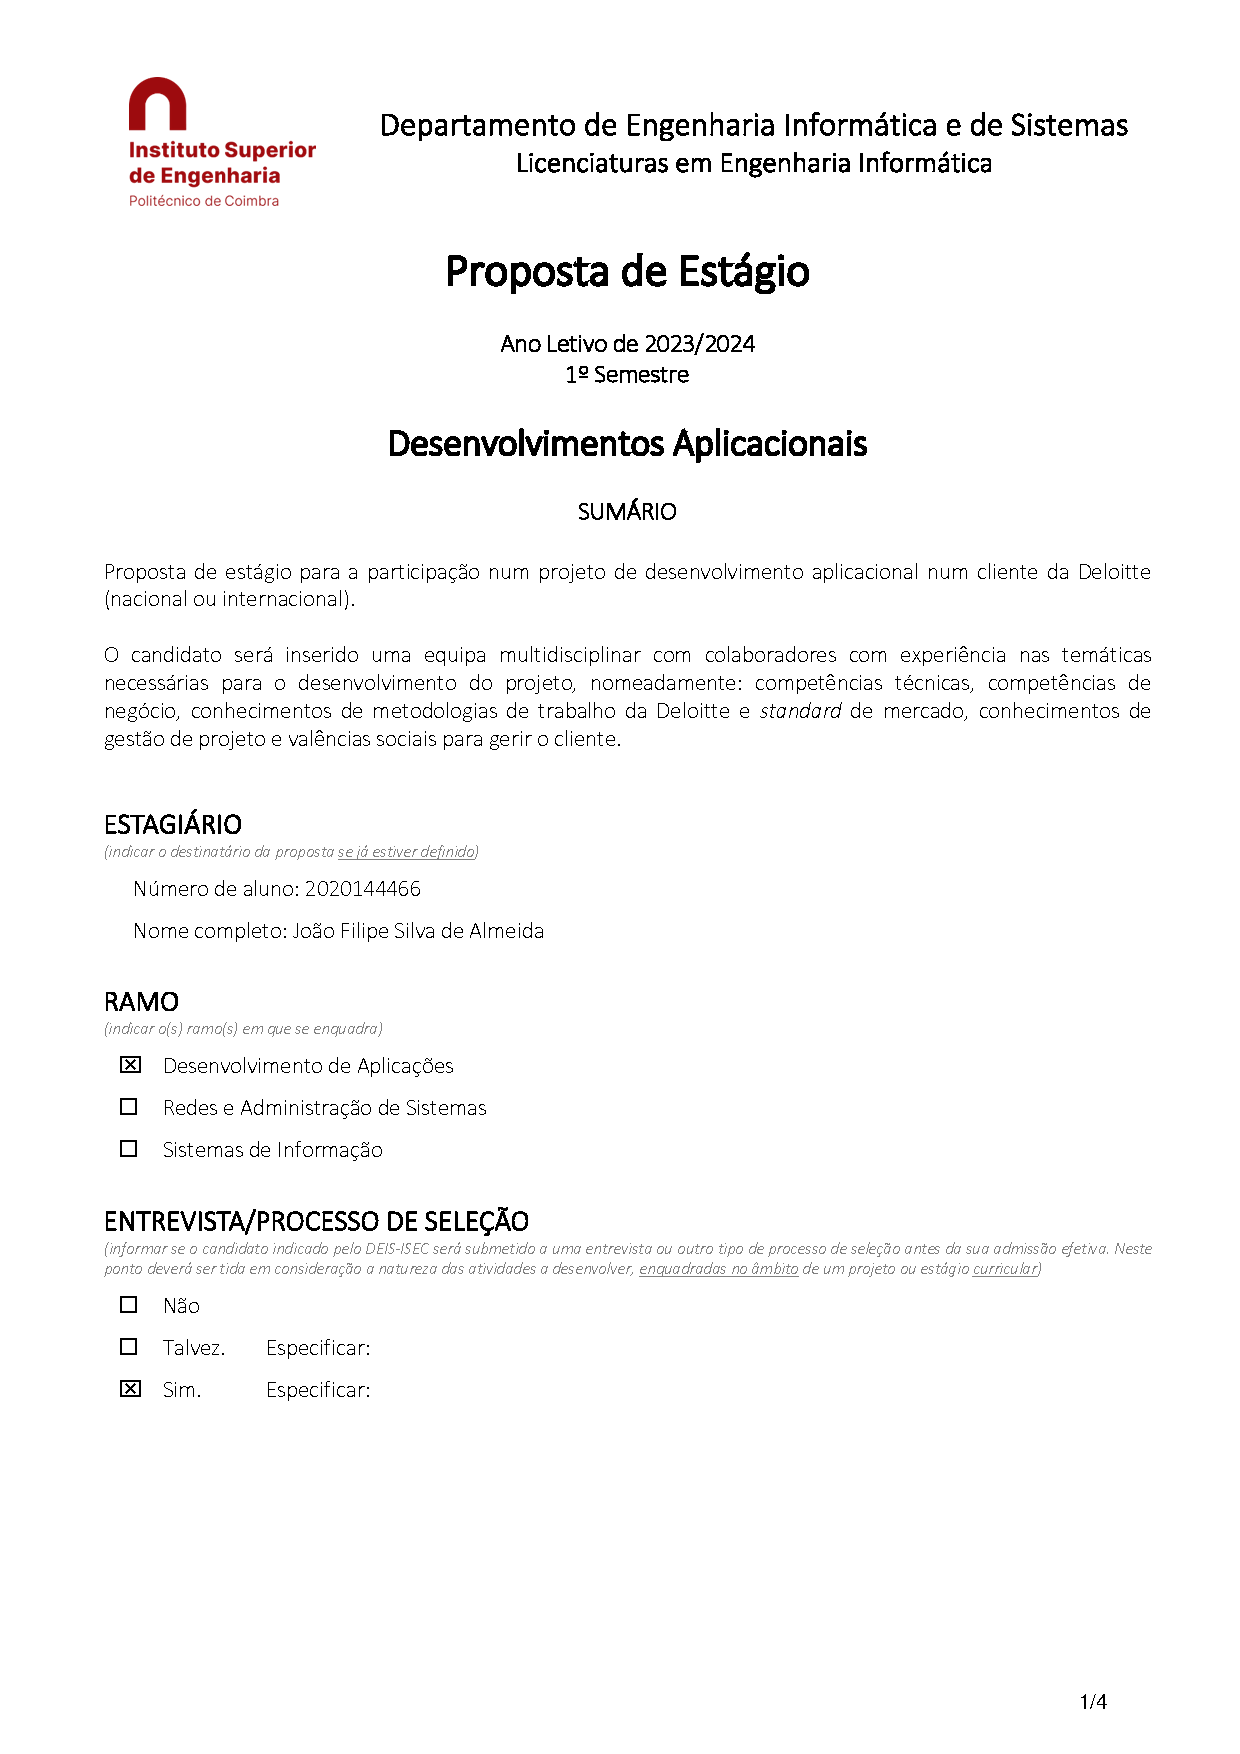
\includegraphics[page=1,scale=0.724]{./imgs/Proposta_Estágio_João_Almeida.pdf}

        \includepdf[scale=0.9,pages=2-,pagecommand={}]{./imgs/Proposta_Estágio_João_Almeida.pdf}
    \end{center}


  \section{Mapa de Gantt das Formações do Estágio}\label{anexo_formacoes}

\pagenumbering{arabic}% resets `page` counter to 1
\renewcommand*{\thepage}{B\arabic{page}}

\begin{figure}[htbp]
    \centering

    \def\pgfcalendarweekdayletter#1{%
      \ifcase#1\tiny{M}\or \tiny{T}\or \tiny{W}\or \tiny{T}\or \tiny{F}\or \tiny{S}\or \tiny{S}\fi%
    }

    % https://texdoc.org/serve/pgfgantt/0
    % https://tex.stackexchange.com/questions/473597/gantt-chart-looks-squished-because-small-time-slot-unit
    % https://tex.stackexchange.com/questions/570631/gantt-chart-bar-label-spacing-issues
    
    % hgrid,
    % vgrid,
    % x unit=2mm,
    % time slot format=isodate,
    % time slot unit=day,
    % calendar week text={\tiny{W\currentweek{}}}

    \begin{ganttchart}[
        hgrid,
        vgrid,
        x unit=2.1mm,
        time slot format=isodate,
        time slot unit=day,
        calendar week text={\tiny{W\currentweek{}}},
        bar label node/.style={text width=2.7cm,
          align=right,
          anchor=east,
          font=\footnotesize\raggedleft}
    ]{2023-09-19}{2023-11-13}
        \gantttitlecalendar{year, month=shortname, week, weekday=letter} \\
        % Activities
        \ganttbar[bar/.append style={fill=color1, opacity=0.8}]{PL/SQL\ \ \ \ }{2023-09-18}{2023-09-20} \\
        \ganttbar[bar/.append style={fill=color2, opacity=0.8}]{Java}{2023-09-20}{2023-09-22} \\
        \ganttbar[bar/.append style={fill=color3, opacity=0.8}]{Excel}{2023-09-25}{2023-09-26} \\
        \ganttbar[bar/.append style={fill=color4, opacity=0.8}]{SQL e modelização}{2023-09-27}{2023-09-28} \\
        \ganttbar[bar/.append style={fill=color1, opacity=0.8}]{Boas práticas de desenvolvimento}{2023-09-29}{2023-09-29} \\
        \ganttbar[bar/.append style={fill=color2, opacity=0.8}]{Banca}{2023-10-02}{2023-10-02} \\
        \ganttbar[bar/.append style={fill=color3, opacity=0.8}]{Seguros}{2023-10-02}{2023-10-02} \\
        \ganttbar[bar/.append style={fill=color4, opacity=0.8}]{Agile/Scrum}{2023-10-03}{2023-10-03} \\
        \ganttbar[bar/.append style={fill=color1, opacity=0.8}]{Getting Things Done}{2023-10-03}{2023-10-03} \\
        \ganttbar[bar/.append style={fill=color2, opacity=0.8}]{CMMI}{2023-10-03}{2023-10-03} \\
        \ganttbar[bar/.append style={fill=color3, opacity=0.8}]{Formação de testes}{2023-10-04}{2023-10-06} \\
        \ganttbar[bar/.append style={fill=color4, opacity=0.8}]{OutSystems}{2023-10-09}{2023-10-20} \\
        \ganttbar[bar/.append style={fill=color1, opacity=0.8}]{Azure}{2023-10-23}{2023-11-13} \\
        %\ganttmilestone[fractional xshift=1/2]{Test}{2023-09-20}
    \end{ganttchart}
    
    \caption{Mapa de Gantt das formações}\label{fig:tempoform}
\end{figure}    

  \section{Requisitos Funcionais dos Scripts de Python}\label{sec:Req_func_python_anexo}

    \pagenumbering{arabic}% resets `page` counter to 1
    \renewcommand*{\thepage}{C\arabic{page}}

    \begin{table}[htbp] % htbp
        \centering
        \begin{tblr}{
            % example for tblr: https://tex.stackexchange.com/questions/603349/tabularray-and-new-command-for-multicolumn-cells
            % another example: https://tex.stackexchange.com/questions/605676/tabularray-how-to-control-the-vertical-alignment-of-the-cells-contents
            hlines={lightgray}, vlines={lightgray},
            width = \linewidth,% total width set to width available
            %rows = {c,m}, % c/l/r aligns horizontally, m/t/b aligns vertically, aligns all rows
            colspec={X[1,l,m] X[5,l,m]}, % the first number is the size % the second is c for center, l for left
        }
        % \textbf{Tempo trabalhado}
            \textbf{ Nome } & \textbf{REQ-02 --- Análise de Utilizadores Inativos em GenerateMRCEmailProcess} \\
            Resumo                  & Os utilizadores devem conseguir analisar processos \texttt{GenerateMRCEmailProcess} num ficheiro Excel, identificando e ignorando automaticamente no Service Center aqueles com utilizadores inativos na plataforma Atlas. \\

            Descrição               & O sistema deve permitir a análise de processos \texttt{GenerateMRCEmailProcess} presentes num ficheiro Excel. Utilizando a plataforma Atlas, deve identificar os processos com utilizadores inativos e ignorá-los automaticamente na plataforma Service Center. \\

            Requisitos Relacionados & -- \\

        \end{tblr}
        \caption{Requisito funcional \textit{Análise de Utilizadores Inativos em GenerateMRCEmailProcess}}
        \label{tab:req2_py}
    \end{table}

    \begin{table}[htbp] % htbp
        \centering
        \begin{tblr}{
            % example for tblr: https://tex.stackexchange.com/questions/603349/tabularray-and-new-command-for-multicolumn-cells
            % another example: https://tex.stackexchange.com/questions/605676/tabularray-how-to-control-the-vertical-alignment-of-the-cells-contents
            hlines={lightgray}, vlines={lightgray},
            width = \linewidth,% total width set to width available
            %rows = {c,m}, % c/l/r aligns horizontally, m/t/b aligns vertically, aligns all rows
            colspec={X[1,l,m] X[5,l,m]}, % the first number is the size % the second is c for center, l for left
        }
        % \textbf{Tempo trabalhado}
            \textbf{ Nome } & \textbf{REQ-04 --- Interrupção Controlada do Script} \\

            Resumo                  & Os utilizadores devem conseguir interromper controladamente a execução do script em qualquer momento, utilizando a combinação de teclas CTRL + ALT + S. \\

            Descrição               & O sistema deve possibilitar ao utilizador interromper a execução do script imediatamente em qualquer ponto, utilizando a combinação de teclas CTRL + ALT + S. \\

            Requisitos Relacionados & -- \\

        \end{tblr}
        \caption{Requisito funcional \textit{Interrupção Controlada do Script}}
        \label{tab:req4_py}
    \end{table}

    \begin{table}[htbp] % htbp
        \centering
        \begin{tblr}{
            % example for tblr: https://tex.stackexchange.com/questions/603349/tabularray-and-new-command-for-multicolumn-cells
            % another example: https://tex.stackexchange.com/questions/605676/tabularray-how-to-control-the-vertical-alignment-of-the-cells-contents
            hlines={lightgray}, vlines={lightgray},
            width = \linewidth,% total width set to width available
            %rows = {c,m}, % c/l/r aligns horizontally, m/t/b aligns vertically, aligns all rows
            colspec={X[1,l,m] X[5,l,m]}, % the first number is the size % the second is c for center, l for left
        }
        % \textbf{Tempo trabalhado}
            \textbf{ Nome } & \textbf{REQ-03 --- Análise de Documentos em UploadDocuments\_V4} \\

            Resumo                  & Os utilizadores devem conseguir analisar processos \texttt{UploadDocuments\_V4} num ficheiro Excel, verificando a existência de documentos associados ao "ContextId" na base de dados do MongoDB e registando informações no Excel. \\

            Descrição               & O sistema deve permitir a análise dos processos \texttt{UploadDocuments\_V4} num ficheiro Excel. Deve verificar se o "ContextId" possui documentos na base de dados de Produção do MongoDB. Em caso negativo, deve assinalar no Excel a mensagem "Contract does not exist in Mongo" e prosseguir. Se existirem documentos com URIs, deve assinalar no Excel com o comentário "Document in Mongo". \\

            Requisitos Relacionados & -- \\

        \end{tblr}
        \caption{Requisito funcional \textit{Análise de Documentos em UploadDocuments\_V4}}
        \label{tab:req3_py}
    \end{table}

    \begin{table}[htbp] % htbp
        \centering
        \begin{tblr}{
            % example for tblr: https://tex.stackexchange.com/questions/603349/tabularray-and-new-command-for-multicolumn-cells
            % another example: https://tex.stackexchange.com/questions/605676/tabularray-how-to-control-the-vertical-alignment-of-the-cells-contents
            hlines={lightgray}, vlines={lightgray},
            width = \linewidth,% total width set to width available
            %rows = {c,m}, % c/l/r aligns horizontally, m/t/b aligns vertically, aligns all rows
            colspec={X[1,l,m] X[5,l,m]}, % the first number is the size % the second is c for center, l for left
        }
        % \textbf{Tempo trabalhado}
            \textbf{ Nome } & \textbf{REQ-05 --- Pintar Colunas com Erros de Roxo para Análise Manual} \\

            Resumo                  & Os utilizadores devem conseguir identificar visualmente colunas com erros, pintadas a roxo no Excel, para posterior análise manual. \\

            Descrição               & O sistema deve pintar de roxo as colunas no Excel que apresentem erros, facilitando a identificação para análise manual. O script deve continuar a execução após esta identificação. \\

            Requisitos Relacionados & REQ-01, REQ-02, REQ-03 \\

        \end{tblr}
        \caption{Requisito funcional \textit{Pintar Colunas com Erros de Roxo para Análise Manual}}
        \label{tab:req5_py}
    \end{table}

  \section{Scripts de Python}\label{sec:scripts}

    \pagenumbering{arabic}% resets `page` counter to 1
    \renewcommand*{\thepage}{D\arabic{page}}

    
    \definecolor{dkgreen}{rgb}{0,0.6,0}
    \definecolor{gray}{rgb}{0.5,0.5,0.5}
    \definecolor{mauve}{rgb}{0.58,0,0.82}
    
    \lstset{frame=tb,
      language=Python,
      aboveskip=3mm,
      belowskip=3mm,
      showstringspaces=false,
      columns=flexible,
      basicstyle={\small\ttfamily},
      postbreak=\mbox{\textcolor{red}{$\hookrightarrow$}\space},
      breaklines=true,
      numbers=none,
      numberstyle=\tiny\color{gray},
      numbers=left,
      keywordstyle=\color{blue},
      commentstyle=\color{dkgreen},
      stringstyle=\color{mauve},
      breaklines=true,
      tabsize=3
    }



    \subsection{\texttt{sdcprocesses-ActiveLoops.py}}\label{secsec:sdcprocesses}

        \lstinputlisting{src/scripts/sdcprocesses-ActiveLoops.py}


    \subsection{\texttt{mrcprocesses.py}}\label{secsec:mrcprocesses}

        \lstinputlisting{src/scripts/mrcprocesses.py}


    \subsection{\texttt{4VDocumentsprocesses.py}}\label{secsec:4VDocumentsprocesses}

        \lstinputlisting{src/scripts/4VDocumentsprocesses.py}


    \subsection{\texttt{requirements.txt}}\label{secsec:requirements}

        \lstinputlisting{src/scripts/requirements.txt}




\let\thefootnote\relax\footnotetext{Este relatório foi gerado utilizando LaTeX. Os arquivos-fonte estão disponíveis em \href{https://github.com/Yeshey/DeloitteInternshipReport-Latex}{https://github.com/Yeshey/DeloitteInternshipReport-Latex}.}

\end{document}
